\section{Regularised estimation of sparse networks and covariances}
\label{app:networks}

Detailed review in the \vignette{03-2-covariance-network-estimation.html}{network-inference vignette}.

\begin{itemize}
  \item estimand: the precision \(\boldsymbol{\Omega}_{j}\) of the within-type Gaussian; zeros are conditional
        independences, and partial correlations are \(-\omega_{gg'}/\sqrt{\omega_{gg}\omega_{g'g'}}\)
  \item three thresholds that are often conflated
  \begin{itemize}
    \item the penalised estimator exists: with an off-diagonal penalty, the graphical lasso has a unique solution
          for any \(\lambda>0\) once every variance is positive, even when \(G>n\)
          \cite{carterExistencePenalisedLikelihood2025}
    \item the unpenalised maximum-likelihood estimate needs \(n>G\)
          \cite{chiquetContributionsSparseMethods2015}; on a fixed graph, the refit under its zeros needs \(n\) above
          the graph's maximum-likelihood threshold \cite{dahlMaximumLikelihoodEstimation2005}
    \item the graph is recovered when \(n\asymp d^{2}\log G\) for maximum degree \(d\), under irrepresentability,
          bounded eigenvalues and a minimum signal; these conditions cannot be checked on real data, and they
          fail on models derived from gene expression
          \cite{chiquetContributionsSparseMethods2015,heinävaaraInconsistencyℓ1penalisedSparse2016}
  \end{itemize}
  \item estimators
  \begin{itemize}
    \item graphical lasso \cite{friedmanSparseInverseCovariance2008,mazumderGraphicalLassoNew2011}: with a penalised
          diagonal the fitted variances become \(S_{gg}+\lambda\), which biases the precision and the partial
          correlations without moving the empty-graph threshold \(\max_{g\neq g'}|R_{gg'}|\); our pipeline fits the
          correlation matrix with \texttt{glasso(penalize.diagonal = FALSE)}
    \item partial-correlation graphical lasso: penalises the partial correlations only, is scale invariant, and
          alternates between the partial correlations and the diagonal
          \cite{carterExistenceOptimisationPartial2025}
    \item joint sparse regression (SPACE): node-wise regressions made symmetric, with the diagonal re-estimated
          from residual variances; better hub recovery \cite{pengPartialCorrelationEstimation2009}
    \item D-trace loss: an alternative to the likelihood with a weaker irrepresentability condition
          \cite{zhangSparsePrecisionMatrix2014}
    \item de-sparsified graphical lasso with entrywise inference and global false discovery rate control
          \cite{jankovaConfidenceIntervalsHighdimensional2015,liuGaussianGraphicalModel2013,zhangSILGGMExtensivePackage2018},
          on nonparanormal scores \cite{liuNonparanormalSemiparametricEstimation2009}
    \item Poisson--log-normal network: the precision of a latent Gaussian behind Poisson counts, free of the
          sampling noise that attenuates count correlations \cite{chiquetVariationalInferenceSparse2018}
    \item dense shrinkage: correlations shrunk towards zero with a closed-form intensity, variances kept;
          positive definite for any \(n\ge2\) and any \(G\) once every variance and the intensity are positive
          \cite{schäferShrinkageApproachLargescale2005}
  \end{itemize}
  \item several cell types
  \begin{itemize}
    \item shrunk covariances \(\alpha S^{(j)}+(1-\alpha)\bar S\), shared support (group lasso) or sign-coherent
          edges (cooperative lasso)
          \cite{chiquetInferringMultipleGraphical2011,danaherJointGraphicalLasso2012,chiquetSparsitySigncoherentGroups2012}
    \item differential networks estimated directly, without either network
          \cite{yuanDifferentialNetworkAnalysis2017}
    \item fusion pulls rare types towards the dominant network, and removes the covariance differences that
          DeCovarT uses to separate types
  \end{itemize}
  \item penalty selection: extended BIC \cite{foygelExtendedBayesianInformation2010}, StARS
        \cite{liuStabilityApproachRegularization2010}, thresholded adaptive validation
        \cite{laszkiewiczThresholdedAdaptiveValidation2021}, or a graphical horseshoe instead of a path
        \cite{liGraphicalHorseshoeEstimator2019}
\end{itemize}

\section{A covariance-driven statistical simulator}
\label{app:simulator}

\subsection{Synthetic network simulation}
\label{sec-synthetic-network}

Three families of random graphs generate the skeletons of the precision matrices.
\begin{itemize}
    \item generalised random graph: given an arbitrary degree distribution, edges are placed so that
        the graph is no longer forced to be homogeneous
        \cite{newmanRandomGraphsModels2002}
    \item Preferential attachment: nodes are added one at a time and connect preferentially to
        well-connected nodes \cite{barabasiEmergenceScalingRandom1999,newmanStructureDynamicsNetworks2011}.
        The degree distribution follows a power law, which produces hubs; such scale-free graphs are often
        assumed for biological networks, although the evidence is debated
        \cite{lima-mendezPowerfulLawPower2009,broidoScalefreeNetworksAre2019}.
    \item Stochastic block model (affiliation model): a latent label assigns each node to a community,
        and edges are more likely within a block than between blocks
        \cite{hollandStochasticBlockmodelsFirst1983}.
\end{itemize}

Signed weights on the edges give a symmetric matrix \(\boldsymbol{W}\), which is turned into a
\gls{posdef} precision by the affine spectrum transformation
\begin{equation}
  \boldsymbol{\Omega}=\boldsymbol{W}+\bigl(\lvert\lambda_{\min}(\boldsymbol{W})\rvert+u\bigr)\mathbf{I}_{G},
  \qquad u>0,
  \label{eq-affine-spectrum-transformation}
\end{equation}
which keeps the off-diagonal support and signs (Theorem~\ref{supp-thm-affine}) and sets the
smallest eigenvalue of \(\boldsymbol{\Omega}\) to \(u\) \cite{chiquetVariationalInferenceSparse2018}.



\begin{theorem}[Invariance of the spectrum function by affine
transformation]
    \label{supp-thm-affine}

    Let $X$ be any square matrix, and consider the affine transformation:

    \[
        Y = aX + bI
    \]

    with $a$ and $b$ positive scalars, and $I$ the identity matrix. Then
    $Y$ has the same eigenvectors as $X$, and every eigenvalue
    $\lambda$ of $X$ becomes $a\lambda+b$: the \gls{spectrum} is scaled by $a$ and shifted by $b$.
\end{theorem}



\section{Review of deconvolution algorithms leveraging cell-type-specific variances}
\label{app:review}

Detailed review in the \vignette{05-1-review-distribution-aware.html}{review vignette}.

\subsection{Measurement versus expression models}

\begin{itemize}
  \item a measurement model \(p(\boldsymbol{x}\mid\boldsymbol{\lambda})\) is separated from an expression model
        \(p(\boldsymbol{\lambda})\); for UMI counts \(x_{gc}\sim\mathrm{Poisson}(s_{c}b_{g}m_{gc})\), and the capture
        \(b_{g}\) cancels within one protocol but not between a single-cell reference and a bulk library
        \cite{sarkarSeparatingMeasurementExpression2021}
  \item overdispersion in UMI data is an expression property plus extrinsic noise, so a moment-based method needs no
        zero-inflated layer
  \item the size factor splits into a biological and a technical part; normalising by total counts removes the
        biological part, including cell size \cite{fangExtrinsicBiologicalStochasticity2025}
  \item early methods fitted unlogged microarray intensities of sorted populations
        \cite{abbasDeconvolutionBloodMicroarray2009,shen-orrCellTypeSpecific2010,lahdesmakiSilicoMicrodissectionMicroarray2005},
        whose only second moment was a between-replicate variance
\end{itemize}

\subsection{Errors in variables and moment estimators}
\label{app:eiv}

\begin{itemize}
  \item errors-in-variables reading: every method fits \(\boldsymbol{y}_{\cdot i}=\hat{\boldsymbol{\mu}}\boldsymbol{p}_{\cdot i}+\boldsymbol{e}_{i}\) with latent
        profiles \(\boldsymbol{x}_{\cdot j,i}=\boldsymbol{\mu}_{\cdot j}+\boldsymbol{u}_{\cdot j,i}\) and reference error
        \(\hat{\boldsymbol{\mu}}=\boldsymbol{\mu}+\boldsymbol{v}\); \emph{RNA-Sieve} and \emph{MEAD} model \(\boldsymbol{v}\)
        \cite{erdmann-phamLikelihoodbasedDeconvolutionBulk2021,xieStatisticalInferenceCell2026}, the others plug
        \(\hat{\boldsymbol{\mu}}\) in
  \item the error law is parametric (DeCovarT, \emph{RCTD}), asymptotic (\emph{RNA-Sieve}, \emph{MEAD}) or given by its
        first two moments only (\emph{DECALS}, \emph{MuSiC}, \emph{DWLS}, \emph{deMixSC})
        \cite{agrestiFoundationsLinearGeneralized2015}; the classical assumptions fail because the error variance
        \(\sum_{j}p_{ji}^{2}\boldsymbol{\Sigma}_{j}\) (DeCovarT) or the Poisson mean (\emph{RCTD}) depends on \(\boldsymbol{p}\)
  \item our reading: \(\boldsymbol{u}\) is a Berkson error weighted by \(p_{ji}\); \(\boldsymbol{v}\) is a classical error that
        DeCovarT ignores
  \item weighted NNLS (\emph{MuSiC}, \emph{DWLS}, \emph{deMixSC}) and \emph{Unico} are generalised-method-of-moments
        estimators: point estimates, and no interval without a variance model, a sandwich or a resampling unit
        \cite{wangBulkTissueCell2019,tsoucasAccurateEstimationCelltype2019,chenUnicoUnifiedModelCell2025}
  \item \emph{Unico}'s conditions are per bulk sample, because each sample has its own law: the first matches the model
        mean \(\boldsymbol{p}_{\cdot i}^{\top}\boldsymbol{\mu}_{g\cdot}\) with \(y_{gi}\), the second the model variance
        \(\boldsymbol{p}_{\cdot i}^{\top}\boldsymbol{\Gamma}_{g}\boldsymbol{p}_{\cdot i}+\tau_{g}^{2}\) with the squared residual; the estimate minimises the
        quadratic form of these \(2N\) conditions in the inverse of their covariance, diagonal for independent samples,
        hence weighted least squares \cite[pp.~13--14]{chenUnicoUnifiedModelCell2025}; see \cite{hansenLargeSampleProperties1982}
        for the general estimator
  \item \emph{deMixSC} \cite{guoDeMixSCDeconvolutionFramework2023}: weighted NNLS with weight
        \(w_{gi}^{-1}=\hat y_{gi}^{2}+(y_{gi}-\hat y_{gi})^{2}+2\), combining the \emph{DWLS} relative-error term and
        \emph{MuSiC}'s residual variance; genes discordant between matched bulk and pseudo-bulk are down-weighted by
        \(a^{-2}=10^{-6}\); point estimates
\end{itemize}

\subsection{Cell-type-specific moments given the composition}
\label{app:cts}

\begin{itemize}
  \item with \(\{\boldsymbol{p}_{\cdot i}\}\) known, the unknowns become the type moments or the sample-level profiles
  \item \emph{CSNet}: gene-wise least squares for the means, regression of residual products on \(p_{ji}^{2}\) for
        each covariance entry, then SCAD on the correlation; a marginal co-expression graph that needs many bulks
        of varying composition \cite{suEstimatingCellTypeSpecificGene2024}
  \item \emph{bMIND}: a \(J\times J\) covariance across types within each gene, with an inverse-Wishart prior from
        single-cell summaries; proportions fixed beforehand \cite{wangBayesianEstimationCelltypespecific2020}
  \item \emph{EPIC-unmix} re-centres that prior on a first-step posterior, using the target samples twice
        \cite{tangCellTypespecificInference2025}
  \item \emph{Unico}: proportions given, \(\operatorname{Var}(y_{gi})=\boldsymbol{p}_{\cdot i}^{\top}\boldsymbol{\Gamma}_{g}\boldsymbol{p}_{\cdot i}+\tau_{g}^{2}\) with a
        \(J\times J\) covariance \(\boldsymbol{\Gamma}_{g}\) across cell types, fitted by moments; sample-level profiles by a
        conditional expectation \cite{chenUnicoUnifiedModelCell2025}
  \begin{itemize}
    \item inputs are the bulk matrix and proportions estimated beforehand; single cells serve only to build benchmark
          pseudo-bulks with known profiles \cite[pp.~11 and~17]{chenUnicoUnifiedModelCell2025}; \emph{Bisque}'s unpaired
          mode, by contrast, matches the mean and variance of each bulk gene across samples with those of single-cell
          pseudo-bulks \cite[p.~10]{jewAccurateEstimationCell2020}
    \item fit: non-negative means by the constrained least-squares solver \texttt{pcls}, variances and covariances by
          COBYLA with a small \(L_{2}\) penalty, samples beyond two standard deviations dropped, weights updated over two
          (means) and three ((co)variances) iterations \cite[p.~14]{chenUnicoUnifiedModelCell2025}
    \item our remark: since \(\mathbf{1}^{\top}\boldsymbol{p}_{\cdot i}=1\),
          \(\boldsymbol{p}_{\cdot i}^{\top}(\boldsymbol{\Gamma}_{g}+c\mathbf{1}\mathbf{1}^{\top})\boldsymbol{p}_{\cdot i}=\boldsymbol{p}_{\cdot i}^{\top}\boldsymbol{\Gamma}_{g}\boldsymbol{p}_{\cdot i}+c\), so the constant
          part of \(\boldsymbol{\Gamma}_{g}\) and \(\tau_{g}^{2}\) are identified only together; the choice still moves the
          profiles of Theorem~1 and the cross-type correlations
    \item the von Neumann entropy of the cross-type correlation only stratifies genes at the median for evaluation; it
          does not filter them \cite[pp.~19--20]{chenUnicoUnifiedModelCell2025}
  \end{itemize}
  \item \emph{imply}: repeated bulk samples of one subject share one reference; stage I estimates proportions by
        \(\nu\)-support vector regression on a population signature, stage II fits per gene the linear mixed model
        \(\mathbb{E}(y_{g,ni})=\sum_{j}(m_{gj}+\beta_{gj}z_{n}+u_{gjn})\hat\theta_{j,ni}\) by REML, with a subject random effect
        \(u_{gjn}\), and predicts the subject reference \(r_{gjn}=\hat m_{gj}+z_{n}\hat\beta_{gj}+\hat u_{gjn}\); stage III refits
        the proportions by non-negative least squares with that reference \cite[pp.~4--5]{mengImplyImprovingCelltype2024}
  \begin{itemize}
    \item our remarks: stage II is the gene-wise BLUP of the linear-mixed-model reading of Section~\ref{sec:wiener}, with
          one random effect per subject; the joint stage-III objective separates into one NNLS per sample; the same
          samples build the reference and are deconvolved with it, and no interval is returned
    \item our perspective: a negative-binomial mixed model with an identity link on the mixture mean would carry the
          same structure to counts
          % TODO-cite: Brooks et al. 2017, glmmTMB, The R Journal 9(2):378-400, doi:10.32614/RJ-2017-066 (not in decovart_library.bib)
  \end{itemize}
  \item a \(J\times J\) covariance within a gene and DeCovarT's \(G\times G\) covariance within a type answer different
        questions; no reviewed method fits both
\end{itemize}

\subsection{Bayesian approaches}

\begin{itemize}
  \item \emph{BLADE}: log-normal profiles with priors centred on single-cell moments, variational inference
        \cite{andrade-barbosaBayesianLogNormalDeconvolution2021}
  \item \emph{BEDwARS}: log-scale profiles around a noisy reference, Metropolis--Hastings, a cohort-level signature
        \cite{ghaffariBEDwARSRobustBayesian2023}
  \item \emph{BayesPrism}: multinomial counts with a single-cell prior, Gibbs sampling, transcript fractions
        \cite{chuCellTypeGeneExpression2022}
  \item \emph{DSection}: Gaussian on linear intensities with a Dirichlet prior centred on a prior guess of the
        proportions \cite{erkkilaProbabilisticAnalysisGene2010}
  \item \emph{gnSPADE}: reference-free topic model whose network prior acts on labels, not on expression
        \cite{xieGnSPADEIncorporatingGene2026}
  \item \emph{DeconV}: zero-inflated Poisson or negative-binomial counts fitted to the single-cell reference, then a bulk
        \(y_{gi}\sim\mathrm{Poisson}(K_{i}\sum_{j}p_{ji}\theta_{gj})\) with \(\theta_{gj}\sim\mathrm{Gamma}(\hat\alpha_{gj},\hat\beta_{gj})\), or
        \(\mathrm{NB}(K_{i}\sum_{j}p_{ji}r_{gj},P_{g})\), and \(\boldsymbol{p}_{\cdot i}\sim\mathrm{Dirichlet}(\boldsymbol{N})\); intervals read from the fitted
        Dirichlet \cite[pp.~6--7]{gynterDeconvProbabilisticCellType2023}
  \begin{itemize}
    \item our remark: a sum of Poisson cells is Poisson, and a sum of negative binomials is negative binomial only because
          \(P_{g}\) is shared across types; with a type-specific \(P_{gj}\) the bulk law is a finite convolution, as in
          \emph{DeMixNB}; the Gamma rate, drawn once per bulk, adds a variance term quadratic in \(p_{ji}\)
    \item \emph{deMixSC} writes the bulk as the same sum over cells but with an additive noise of unspecified law, fitted by
          weighted NNLS \cite{guoDeMixSCDeconvolutionFramework2023}; it is not a negative-binomial convolution
  \end{itemize}
  \item \emph{BLEND}: multinomial reads whose type-\(j\) profile in sample \(i\) is the convex combination
        \(\sum_{m}\psi_{j,i,m}\boldsymbol{\Phi}_{j,m}\) of \(M_{j}\) observed references, Dirichlet priors on the fractions and the
        weights, Gibbs sampling or EM for the posterior mode; the fractions are RNA fractions, converted with cell sizes
        \cite[pp.~8--10]{huangBLENDProbabilisticCellular2024}; compared with the Wiener filter in
        Appendix~\ref{app:wiener-blend}
\end{itemize}

\subsection{Semi-reference and reference-free methods}

\begin{itemize}
  \item one unknown component: \emph{DeMix} and \emph{DeMixT} mix \(\log_{2}\)-normal components on the raw scale
        \cite{ahnDeMixDeconvolutionMixed2013,wangTranscriptomeDeconvolutionHeterogeneous2018}; \emph{DeMixNB} uses an
        exact negative-binomial convolution \cite{montierthDeconvolutionSparsecountRNA2025}; \emph{BayICE} mixes on the
        log scale, a mean regression rather than a convolution \cite{taiBayiceBayesianHierarchicalModel2021};
        \emph{ISOpureR} is a multinomial with a Dirichlet-shrunk tumour profile
        \cite{anghelISOpureRImplementationComputational2015}
  \item reference-free with co-expression structure: \emph{DSSC} fits similarity kernels built from the same bulk
        \cite{wangDeconvolutionBulkGene2024}; \emph{GSNMF+} regularises the signature with a co-expression graph
        \cite{liAugmentedGSNMFModel2025}; \emph{swCAM} penalises sample-specific deviations with a nuclear norm, which
        implies a low-rank gene covariance \cite{chenSwCAMEstimationSubtypespecific2022}; all three use a Frobenius
        loss and ignore the mean--variance relationship of counts
\end{itemize}

\subsection{Optimisation when the likelihood is not explicit}
\label{app:review-optim}

\begin{itemize}
  \item the bulk density is explicit when the cell-type profiles are Gaussian on the linear scale, as in DeCovarT; it is not
        when the components are log-normal or negative binomial, nor when one component is unknown, as in semi-reference
        methods; three strategies follow, summarised in Table~\ref{tab:review-optim}
  \item first and second moments only: \emph{MEAD} solves a bias-corrected estimating equation in closed form,
        \(\hat{\boldsymbol{\beta}}=(\hat{\boldsymbol{U}}^{\top}\boldsymbol{W}\hat{\boldsymbol{U}}-\hat{\boldsymbol{V}})^{-1}\hat{\boldsymbol{U}}^{\top}\boldsymbol{W}\boldsymbol{y}\), then truncates or constrains the
        negative coefficients and renormalises \cite[pp.~8--10]{xieStatisticalInferenceCell2026}; \emph{DECALS} fits
        constrained ordinary least squares, a quadratic programme solved by the dual active-set method of Goldfarb and
        Idnani, and iterates cell-type covariances estimated across the bulk cohort, whose asymptotic normality in the
        number of genes serves the intervals \cite[pp.~6--9]{caiStatisticalInferenceCelltype2024}; neither needs a
        distribution, and neither provides a likelihood for tests
  \item a likelihood from the central limit theorem: \emph{RNA-Sieve} writes the bulk as a sum of \(n\) cells, Gaussian by the
        central limit theorem, with Gaussian errors on the reference means, and maximises this composite likelihood over the
        proportions, the cell-type means and \(n\) by alternating quadratic programmes and gradient steps, then projects the
        proportions onto the simplex by weighted least squares; the first phase has no convergence guarantee
        \cite[p.~1804 and Supplemental Sect.~S1.6]{erdmann-phamLikelihoodbasedDeconvolutionBulk2021}; the single-cell model
        of Section~\ref{sec:sc-tailored} rests on the same argument, with a fully parametrised Gaussian likelihood maximised
        jointly by profile Newton (Section~\ref{sec:sc-optimisation})
  \item a numerically approximated likelihood
  \begin{itemize}
    \item \emph{DeMix} evaluates the density of a sum of two log-normal components by numerical integration and maximises
          it over all sample proportions jointly with the Nelder--Mead simplex method; at each candidate the tumour
          log-mean and log-variance are sample moments, and the search stops when the proportions change by less than
          1\%; a per-gene search then splits each bulk into its two components, and the two steps alternate
          \cite[p.~1866 and Supplementary Sect.~1.1]{ahnDeMixDeconvolutionMixed2013}
    \item \emph{DeMixT} keeps the numerical integration, a single or a double integral for two or three components, and
          replaces the joint search by iterated conditional modes: sample-wise proportions and gene-wise parameters are
          maximised in turn, each block in parallel, by golden-section search with successive parabolic interpolation
          under box bounds \cite[p.~453 and Transparent Methods]{wangTranscriptomeDeconvolutionHeterogeneous2018}
    \item \emph{DeMixNB} writes the convolution of two negative-binomial components exactly as a finite sum, and
          alternates the same blocks with L-BFGS-B, the proportions bounded to \([0.05,0.95]\), from three random starts
          \cite{montierthDeconvolutionSparsecountRNA2025}
    \item \emph{ISOpureR} maximises a multinomial--Dirichlet posterior by block coordinate descent; each block is fitted by
          Rasmussen's nonlinear conjugate gradient, with the Polak--Ribi\`ere direction and a Wolfe--Powell line search
          (\texttt{cg\_code} in the package source) \cite[pp.~6--7]{anghelISOpureRImplementationComputational2015}
  \end{itemize}
  \item strengths and pitfalls of those algorithms
  \begin{itemize}
    \item Nelder--Mead needs no derivative; it stops when the spread of the objective over the simplex is small, a test
          that is large on a curved region and small on a flat one \cite[Sect.~7.5, pp.~119--124]{kochenderferAlgorithmsOptimization2026}, so a flat
          likelihood ridge can stop it early; with all sample proportions in one simplex, its dimension grows with the
          number of samples (our assessment)
    \item golden-section search and parabolic interpolation are one-dimensional bracketing methods, reliable on a
          unimodal block \cite[Sects.~3.4--3.5, pp.~47--53]{kochenderferAlgorithmsOptimization2026}
    \item iterated conditional modes and block coordinate descent increase the likelihood at every update, but a search
          along coordinates ``can fail to find even a local minimum'' along a diagonal valley
          \cite[Sect.~7.1, p.~114]{kochenderferAlgorithmsOptimization2026}, and the rate is linear when the blocks are coupled; the single-cell
          alternation of Section~\ref{sec:optim-perspective} needed up to 95 updates
    \item nonlinear conjugate gradient: the Polak--Ribi\`ere coefficient
          \(\beta_{k}=\boldsymbol{g}_{k}^{\top}(\boldsymbol{g}_{k}-\boldsymbol{g}_{k-1})/\boldsymbol{g}_{k-1}^{\top}\boldsymbol{g}_{k-1}\) sets the search direction, the step length comes
          from a line search under the strong Wolfe conditions, and \(\beta=\max(\beta_{k},0)\) restarts it along the
          gradient \cite[Sects.~4.4 and 5.2, pp.~65--70 and 79--81]{kochenderferAlgorithmsOptimization2026}
          (\href{https://en.wikipedia.org/wiki/Nonlinear_conjugate_gradient_method}{nonlinear conjugate gradient}); it uses no
          curvature beyond the line search, whereas Newton's method converges quadratically near the optimum
          \cite[Sect.~6.1, pp.~95--97]{kochenderferAlgorithmsOptimization2026}
    \item L-BFGS-B handles box constraints only \cite[Sects.~6.5 and 10.5, pp.~103--106 and 188]{kochenderferAlgorithmsOptimization2026}: in
          \emph{DeMixNB} the sum-to-one constraint is imposed afterwards, and bounds at 0.05 and 0.95 exclude the faces where a
          type is absent; optimising the likelihood of the closure \(\boldsymbol{p}=\boldsymbol{w}/\mathbf{1}^{\top}\boldsymbol{w}\) over the box
          \(\boldsymbol{w}\ge\mathbf{0}\) instead keeps a box solver exact on the closed simplex (Appendix~\ref{app:optim-solvers})
    \item a line search fixes the direction and then the step length, a trust region the step length and then the
          direction \cite[Sects.~4.4--4.5, pp.~65--73]{kochenderferAlgorithmsOptimization2026}; DeCovarT uses the second (Remark~\ref{rem:step-size})
  \end{itemize}
  \item constraint handling not used by those methods: a transformation to unconstrained coordinates, the ILR chart of
        DeCovarT \cite[Sect.~10.3, pp.~185--187]{kochenderferAlgorithmsOptimization2026}; a projection onto the feasible set after each step
        \cite[Sect.~10.5, pp.~188--189]{kochenderferAlgorithmsOptimization2026}, which is proximal gradient when the non-smooth term is the indicator
        of the simplex, since the proximal step of an indicator returns the closest feasible point
        \cite[Example~11.6, p.~228]{kochenderferAlgorithmsOptimization2026}; penalty and augmented-Lagrangian methods, the latter converging without
        driving the penalty to infinity \cite[Sects.~10.9--10.10, pp.~195--199]{kochenderferAlgorithmsOptimization2026}; interior-point methods with a
        logarithmic barrier \cite[Chap.~11, pp.~561--615]{boydConvexOptimization2004}; the KKT conditions at a face
        \cite[Sect.~5.5.3, pp.~243--244]{boydConvexOptimization2004} (Appendix~\ref{app:kkt}); active-set solvers for the mean-only
        quadratic programme and non-negative least squares \cite[Sect.~13.5, pp.~285--287]{kochenderferAlgorithmsOptimization2026}
\end{itemize}

\begin{table}[ht]
  \centering
  \small
  \caption{Optimisation in likelihood- and moment-based deconvolution methods.}
  \label{tab:review-optim}
  \begin{tabularx}{\textwidth}{@{}lYYY@{}}
    \toprule
    Method & Bulk likelihood & Algorithm & Constraints \\
    \midrule
    MEAD & none: first and second moments & closed-form estimating equation & truncation or constrained fit, renormalisation \\
    DECALS & none for the estimate; normal limit in the number of genes for intervals & dual active-set quadratic programme, iterated covariances & inside the quadratic programme \\
    RNA-Sieve & Gaussian composite likelihood from the central limit theorem & alternating quadratic programmes and gradient steps & weighted projection onto the simplex \\
    DeMix & log-normal convolution, numerical integration & Nelder--Mead over all proportions, per-gene search & implicit in the log-normal moments \\
    DeMixT & log-normal convolution, single or double numerical integral & iterated conditional modes, golden section and parabolic interpolation & box bounds \\
    DeMixNB & exact negative-binomial convolution sum & iterated conditional modes, L-BFGS-B & box \([0.05,0.95]\) \\
    ISOpureR & multinomial with Dirichlet priors & block coordinate descent, Polak--Ribi\`ere conjugate gradient & log domain \\
    Unico & none: first two moments of each bulk sample, proportions given & \texttt{pcls} for the means; COBYLA with an \(L_{2}\) penalty for the (co)variances; diagonal weights updated over two and three iterations & non-negative means; samples beyond two standard deviations dropped \\
    DeconV & Poisson or negative binomial given Gamma or log-normal rates, Dirichlet proportions & stochastic gradient in Pyro, clipped Adam with learning-rate decay; only the Dirichlet concentration is fitted on the bulk & Dirichlet support \\
    imply & Gaussian linear mixed model for the subject references; none for the proportions & REML penalised least squares, then non-negative least squares by quadratic programming & non-negativity \\
    BLEND & multinomial given latent fractions and reference weights & Gibbs sampling, or EM for the posterior mode & simplex constraints in the M-step \\
    DeCovarT & explicit Gaussian & trust-region Newton on the ILR chart, or L-BFGS-B on the closure chart & ILR chart and
      restricted fits on faces, or the box \(\boldsymbol{w}\ge\mathbf{0}\) \\
    \bottomrule
  \end{tabularx}
\end{table}

\subsection{Deep-learning deconvolution: where the non-linearity sits}
\label{app:review-deep}

\begin{itemize}
  \item motivation (our perspective): a latent space indexed by pathways, modules or sets of strongly co-expressed
        genes would average out technical effects that act gene by gene, such as transcript length or capture; the
        linear projections of Section~\ref{sec:latent-space} keep the mixture exact, deep networks drop the linearity
        of the projection
  \item a PRISMA systematic review retains 13 deep-learning tools out of 171 records (searched February 2025)
        (Lomas Redondo et al., 2025, pp.~2550--2551)
        % TODO-cite: Lomas Redondo et al. 2025, Comput Struct Biotechnol J 27:2544-2565, doi:10.1016/j.csbj.2025.05.038
  \begin{itemize}
    \item 11 of the 13 are multilayer perceptrons; \emph{Autoptcr} is convolutional, \emph{TAPE} an autoencoder,
          \emph{CONVdeconv} a hybrid with attention (Sect.~3.2.6); 10 of the 12 tools analysed for their data train
          on pseudo-bulks simulated from scRNA-seq
    \item comparisons are mostly against \emph{CIBERSORTx} and \emph{MuSiC} (8 of 13 papers), and only 7 of 13 compare
          with \emph{Scaden}; the gain of \emph{DAISM-DNN} over \emph{Scaden} disappears when both are trained on the
          same calibration data (Sect.~3.2.7)
    \item gaps stated by the authors: limited interpretability, a SoftMax output with a regression loss, transfer of
          one architecture across tissues, dominance of PBMC data, and pseudo-bulk generation that differs between
          studies (Sect.~4)
    \item our remark: a network trained on sums of single cells learns a non-linear inverse of a linear forward
          model, not a non-linear mixture
  \end{itemize}
  \item level 1, between proportions and bulk: \(\hat{\boldsymbol{p}}=f(\boldsymbol{y})\) directly, as in \emph{Scaden}
        \cite{mendenDeepLearningBased2020} and most perceptron-based tools; additivity is no longer modelled, and the
        drawbacks listed in Section~\ref{sec:latent-space} apply
  \item level 2, non-linear projection and linear unmixing in the latent space: \emph{DECIPHER} (Lai et al., 2026) learns a
        domain-constant representation \(\boldsymbol{Z}_{c}\), aligned between simulated and real samples by maximum mean
        discrepancy, and a domain-specific representation \(\boldsymbol{Z}_{s}\), supervised by a domain classifier;
        differentiable non-negative least squares writes \(\boldsymbol{Z}_{c}\) as a combination of cell-type prototypes,
        and the weights are closed to sum to one (Methods, eqs~4--5); replacing this step by a perceptron lowered the
        concordance in its ablation
        % TODO-cite: Lai et al. 2026, DECIPHER, bioRxiv, doi:10.64898/2026.09.24.753940
  \begin{itemize}
    \item our remark: linearity in \(\boldsymbol{Z}_{c}\) is imposed by training on simulated mixtures, not derived, since
          \(f(\sum_{j}p_{j}\boldsymbol{x}_{\cdot j})\neq\sum_{j}p_{j}f(\boldsymbol{x}_{\cdot j})\); its input is log1p-CPM, not counts;
          \emph{DECONVersation} is the analogue with a frozen foundation-model encoder
          \cite{okuDECONVersationSingleCell2026}
  \end{itemize}
  \item level 3, a non-linear technical layer \(\boldsymbol{y}=\mathcal{T}(\boldsymbol{\mu}\boldsymbol{p})+\boldsymbol{e}\), with
        \(\mathcal{T}\) covering capture bias, RNA content, normalisation and the log transform
  \begin{itemize}
    \item \emph{DECODE} removes batch effects by adversarial training between pseudo-bulk and target tissue, then an
          attention-based denoiser trained by contrastive learning on noisy and clean pseudo-bulk pairs separates
          noise features from tissue features before deconvolution \cite{zhaoDecodeDeepLearningBased2026}
    \item \emph{DISSECT} (Khatri et al., 2024) regularises two networks for consistency between the simulated training domain and the
          real target domain
          % TODO-cite: Khatri, Machart & Bonn 2024, Genome Biol 25:112, doi:10.1186/s13059-024-03251-5
    \item our view: this is the level where non-linearity is justified; on counts, with technical bias accounted
          for, the cells add up and the mixture should stay linear
  \end{itemize}
  \item continuous populations (our perspective): \emph{DECODE} deconvolves cell states as well as types
        \cite{zhaoDecodeDeepLearningBased2026}; a latent space could index a continuum of states, and the composition
        of a sample would become a distribution over that space rather than a vector over \(J\) labels; identifiability
        would then need anchors such as reference types, sparsity or pathway constraints
  \item interpretability: unconstrained latent dimensions are not identified with populations and may encode batch,
        donor or other biological axes (our remark); two methods constrain them with prior knowledge
  \begin{itemize}
    \item \emph{DeSide} (Xiong et al., 2024) integrates biological pathways and estimates the non-cancer cell types first, for 16 cell types
          and subtypes in solid tumours; by the account of \emph{iDCF}, pathways enter by element-wise multiplication
          of the expression with pathway annotations
          % TODO-cite: Xiong et al. 2024, DeSide, PNAS 121:e2407096121, doi:10.1073/pnas.2407096121
    \item \emph{iDCF} (Guo et al., 2026) pairs a standard network with a knowledge-based sparse network whose connections are masked by
          pathway definitions (MSigDB) and protein--protein interactions (STRING), and explains each proportion by
          SHAP attributions
          % TODO-cite: Guo et al. 2026, iDCF, PLoS Comput Biol 22(8):e1014727, doi:10.1371/journal.pcbi.1014727
    \item our perspective: such masks are the closest deep-learning counterpart of a module-level likelihood, whose
          covariance would be block-structured by pathways
  \end{itemize}
  \item outside our scope
  \begin{itemize}
    \item \emph{TAPE} (Chen et al., 2022) and \emph{BLUE} also estimate cell-type-specific expression; \emph{DAISM-DNN} and other
          augmentation schemes enlarge the training set
          % TODO-cite: Chen et al. 2022, TAPE, Nat Commun 13:6735, doi:10.1038/s41467-022-34550-9
    \item \emph{scpDeconv} aligns reference and target domains adversarially; our remark: no alignment predicts how
          a disease changes expression or composition, so a reference matched to the condition of the bulk is
          preferable to a broad atlas of conditions
          % TODO-cite: scpDeconv original paper (not retrieved)
    \item benchmarks disagree: with matched, mismatched and mixed lupus and healthy references, the choice of method
          mattered more than reference matching, \emph{DISSECT} performed best, and matching mattered most for
          regression-based methods \cite{zhaoEvaluatingReferencemixtureMatching2026}; in a ten-method benchmark (Malik et al., 2026),
          \emph{MuSiC}, \emph{DWLS} and \emph{BayesPrism} were strongest at baseline, and deep-learning methods varied more
          % TODO-cite: Malik et al. 2026, Comput Biol Chem 126:109370, doi:10.1016/j.compbiolchem.2026.109370
  \end{itemize}
\end{itemize}

\subsection{Caveats shared across methods}

\begin{itemize}
  \item mixing is additive only on a linear scale; methods that mix logarithms fit a different model
  \item count and topic models, and any fit on library-normalised bulk, return transcript fractions; cell
        fractions need the cell sizes \(S_{j}\)
  \item independent cells give weight \(p_{ji}\), a random population profile gives \(p_{ji}^{2}\); a one-donor
        reference identifies only the first
  \item data reuse inflates apparent accuracy: empirical-Bayes re-centring on the target samples, similarity
        graphs built from the bulk being factorised, and priors from the benchmark's own single-cell source
  \item collinear reference means, perfect markers with gene-wise scales, or factorisations without separability
        leave proportions unidentified at any sample size
\end{itemize}

\subsection{Dynamic and mechanistic models of single-cell expression}
\label{app:dynamic}

This subsection expands Section~\ref{sec:dynamic-inference}. Its symbols are local and aligned with the three
main sources in Table~\ref{tab:dynamic-notation}; DeCovarT symbols keep their meaning.
% TODO-cite: Gorin, Vastola, Fang & Pachter 2022, Nat Commun 13:7620, doi:10.1038/s41467-022-34857-7
% TODO-cite: Maugé & Ventre 2026, CardamomOT, PLoS Comput Biol 22(10), doi:10.1371/journal.pcbi.1014838
% TODO-cite: Tang, Jørgensen, Marguerat, Thomas & Shahrezaei 2023, Bioinformatics 39(7):btad395, doi:10.1093/bioinformatics/btad395
% TODO-cite: Sukys & Grima 2025, Nucleic Acids Res 53(7), doi:10.1093/nar/gkaf295

\begin{table}[ht]
  \centering
  \small
  \caption{Symbols of Appendix~\ref{app:dynamic} and their names in the sources. A dash: the quantity is absent.
    Rates are written \(k^{\mathrm{label}}\), indexed by gene \(g\) and, when they vary, by cell \(c\).}
  \label{tab:dynamic-notation}
  \begin{tabularx}{\textwidth}{@{}lYlll@{}}
    \toprule
    Here & Meaning & Gorin et al. & CardamomOT & Tang et al. \\
    \midrule
    \(x^{\mathrm{mol}}_{gc}\); \(x^{\mathrm{N}}_{gc}\), \(x^{\mathrm{M}}_{gc}\) & molecules in cell \(c\) before capture; nascent
      and mature & \(x_{N}\), \(x_{M}\) & \(M_{i}\) (total) & \(X_{ij}\) \\
    \(x_{gc}\) & observed UMI count (article notation) & -- & \(M_{i}\) & \(x_{ij}\) \\
    \(k^{\mathrm{tx}}_{gc}(t)\) & effective transcription rate & \(K(t)\) & -- & -- \\
    \(k^{\mathrm{on}}_{g}\), \(k^{\mathrm{off}}_{g}\), \(k^{\mathrm{syn}}_{g}\) & promoter activation, inactivation;
      synthesis while active & -- & \(k_{\mathrm{on}}\), \(k_{\mathrm{off}}\), \(s_{0}\) & \(k_{\mathrm{on}}\), \(k_{\mathrm{off}}\),
      \(k_{\mathrm{syn}}\) \\
    \(k^{\mathrm{spl}}_{g}\), \(k^{\mathrm{deg}}_{g}\) & splicing; mRNA degradation & \(\beta\), \(\gamma\) & --, \(d_{0}\) &
      --, \(\phi_{i}\) (plus growth) \\
    \(k^{\mathrm{rev}}_{g}\), \(k^{\mathrm{arr}}_{g}\), \(\varsigma_{g}\) & mean reversion, arrival rate and gain of the
      rate process & \(\kappa\), \(a\), \(\theta\) & -- & -- \\
    \(x^{\mathrm{prot}}_{gc}\); \(k^{\mathrm{tl}}_{g}\), \(k^{\mathrm{pdeg}}_{g}\) & protein level; translation, protein
      degradation & -- & \(P_{i}\); \(s_{1}\), \(d_{1}\) & -- \\
    \(\boldsymbol{\Xi}=(\Xi_{gh})\) & regulatory interactions, effect of gene \(h\) on gene \(g\) & -- & \(\theta_{ij}\) & -- \\
    \(\zeta_{c}\) & cell state: type, cycle phase, promoter basin, condition & -- & \(z\) (basin) & -- \\
    \(\upsilon_{c}\) & relative cell size & -- & -- & \(s_{j}\) \\
    \(b_{c}\), \(b_{g}\) & capture efficiency of cell \(c\); of gene \(g\) (article notation) & -- & -- (code: depth
      \(s_{c}\)) & \(b_{j}\) \\
    \(\psi_{g}\) & negative-binomial size, variance \(m+m^{2}/\psi_{g}\) (article notation) & \(\alpha\) (mixture) &
      \(a\) & -- \\
    \bottomrule
  \end{tabularx}
\end{table}

\begin{itemize}
  \item the question: between two conditions or time points, a gene may change because of technical factors
        (capture, depth), the composition \(\boldsymbol{p}(t)\), a new kinetic regime inside a cell type, or a
        combination; the first is a measurement effect, the second the target of deconvolution, the third the target of
        mechanistic models; telling them apart needs several time points and several independent replicates, the
        donors, which form the outer plate of Figure~\ref{fig:dyn-layers}
  \item interpretable and tractable models (Gorin et al., 2022): a model is \emph{tractable} when its count
        distribution, moments or generating function can be computed exactly or at a small numerical cost, and
        \emph{interpretable} when each parameter has a mechanistic meaning, such as a burst frequency, a burst size, a
        degradation rate or a gain; competing hypotheses are written as such models, the experiment that best
        separates their predictions is chosen, and the data refine or reject them (their Fig.~1a)
  \item their model class: a continuous transcription rate \(k^{\mathrm{tx}}_{gc}(t)\) follows a stochastic differential equation,
        mean reversion plus noise, and drives nascent RNA, spliced at rate \(k^{\mathrm{spl}}_{g}\) into mature RNA degraded
        at rate \(k^{\mathrm{deg}}_{g}\); in both cases below the stationary rate is
        \(\mathrm{Gamma}(k^{\mathrm{arr}}_{g}/k^{\mathrm{rev}}_{g},\ \text{scale }\varsigma_{g})\), with mean
        \(\langle k^{\mathrm{tx}}_{g}\rangle=k^{\mathrm{arr}}_{g}\varsigma_{g}/k^{\mathrm{rev}}_{g}\)
  \begin{itemize}
    \item gamma Ornstein--Uhlenbeck (\(\Gamma\)-OU), DNA mechanics: transcription twists the DNA and lowers the rate at the
          first-order rate \(k^{\mathrm{rev}}_{g}\); topoisomerases arrive at rate \(k^{\mathrm{arr}}_{g}\) and raise it by exponential jumps of
          mean \(\varsigma_{g}\)
    \item Cox--Ingersoll--Ross (CIR), regulation: an abundant regulator produced at rate \(k^{\mathrm{arr}}_{g}\) and degraded at
          rate \(k^{\mathrm{rev}}_{g}\); \(k^{\mathrm{tx}}=\varsigma_{g}\times\)(regulator count), with a noise that grows with the rate
  \end{itemize}
  \item four limits (their Fig.~2) on two axes, \(k^{\mathrm{rev}}/(k^{\mathrm{rev}}+k^{\mathrm{spl}}+k^{\mathrm{deg}})\) and the gain ratio
        \(\varsigma/(\varsigma+k^{\mathrm{arr}})\)
  \begin{itemize}
    \item fast reversion or low gain: a rate constant in time and across cells, the constitutive model; nascent and
          mature counts are independent Poisson with means \(k^{\mathrm{tx}}/k^{\mathrm{spl}}\) and \(k^{\mathrm{tx}}/k^{\mathrm{deg}}\)
    \item slow reversion: a rate frozen in each cell but different between cells, the mixture model; mature counts are
          negative binomial with size \(\psi_{g}=k^{\mathrm{arr}}_{g}/k^{\mathrm{rev}}_{g}\)
          % chk: V34b
    \item high gain: the two models part; \(\Gamma\)-OU gives geometric bursts, the usual bursty model, whose mean size we
          read as \(\varsigma_{g}/k^{\mathrm{rev}}_{g}\) at frequency \(k^{\mathrm{arr}}_{g}\); CIR gives an inverse-Gaussian-driven family with
          heavier tails
  \end{itemize}
  \item the two models have the same means, variances, covariances and autocorrelation functions (their Table~1), so no
        summary of the first two moments, and no measurement that averages cells, can separate them; whole joint
        distributions can, and fitting nascent and mature counts together beats either species alone, usually by an
        order of magnitude in Bayes factor (their Fig.~3b); in real data the differences lie near the peaks and in the
        tails of the distributions; DeCovarT, built on two moments per type, sits on the wrong side of this limit for
        mechanism; the limit does not concern composition, which DeCovarT estimates from these two moments
  \item \emph{CardamomOT} (Maugé and Ventre, 2026), a mechanistic model of a regulatory network
  \begin{itemize}
    \item each gene has a two-state promoter in the bursty regime \(k^{\mathrm{on}}\ll k^{\mathrm{off}}\); proteins set the activation rate,
          \(k^{\mathrm{on}}_{g}(\boldsymbol{x}^{\mathrm{prot}})\), through a sigmoid of \(\sum_{h}\Xi_{gh}x^{\mathrm{prot}}_{h}\), and \(k^{\mathrm{off}}_{g}\) is fixed
    \item given proteins, the mRNA count is negative binomial with shape \(k^{\mathrm{on}}_{g}/k^{\mathrm{deg}}_{g}\) and rate
          \(k^{\mathrm{off}}_{g}/k^{\mathrm{syn}}_{g}\): mean \(k^{\mathrm{on}}_{g}k^{\mathrm{syn}}_{g}/(k^{\mathrm{deg}}_{g}k^{\mathrm{off}}_{g})\), Fano factor
          \(1+k^{\mathrm{syn}}_{g}/k^{\mathrm{off}}_{g}\), and \(\psi_{g}=k^{\mathrm{on}}_{g}/k^{\mathrm{deg}}_{g}\), the burst frequency in units of mRNA
          lifetime (their Eq.~3)
          % chk: V34a
    \item over promoter basins the population law is a negative-binomial mixture (their Eq.~4), so multimodality comes
          from regulation; proteins are slow and deterministic, a piecewise-deterministic Markov process, and are
          reconstructed between snapshots by optimal transport with a cost set by the network; the fit needs exact
          time labels and protein degradation rates
    \item inputs are raw total counts, with no nascent--mature split; cells neither proliferate nor die between
          snapshots, so the transport is balanced (their p.~28); network identifiability limits a fit without prior
          structure to about 100 genes (p.~27)
  \end{itemize}
\end{itemize}

\begin{figure}[ht]
  \centering
  \begin{tikzpicture}[>=stealth, font=\small]
    % (a) Gorin et al.: one gene, nascent and mature RNA
    \begin{scope}
      \node[fixedpar] (drv) at (0,0) {\(k^{\mathrm{arr}}_{g},\varsigma_{g},k^{\mathrm{rev}}_{g}\)};
      \node[fixedpar] (rna) at (2.5,0) {\(k^{\mathrm{spl}}_{g},k^{\mathrm{deg}}_{g}\)};
      \node[latent, minimum size=26pt] (ktx) at (0,-1.8) {\(k^{\mathrm{tx}}_{gc}\)};
      \node[obs, minimum size=26pt] (xn) at (0,-3.6) {\(x^{\mathrm{N}}_{gc}\)};
      \node[obs, minimum size=26pt] (xm) at (2.0,-3.6) {\(x^{\mathrm{M}}_{gc}\)};
      \node[eqnote, left=2pt of ktx] (nk) {SDE:\\reversion\\+ noise};
      \node[eqnote, below=3pt of xm] (nm) {Poisson given\\the rate history};
      \draw[->] (drv) -- (ktx);
      \draw[->] (ktx) -- (xn);
      \draw[->] (xn) -- node[eqnote, above] {splicing} (xm);
      \draw[->] (rna) -- (xn);
      \draw[->] (rna) -- (xm);
      \plate[inner sep=6pt]{cellsA}{(nk)(ktx)(xn)(xm)(nm)}{cells \(c\)};
      \plate[inner sep=6pt]{genesA}{(drv)(rna)(cellsA)(cellsA-caption)}{one gene \(g\), steady state};
      \node[panellabel] at ([yshift=2pt]genesA.north west) {(a) Gorin et al.};
    \end{scope}
    % (b) CardamomOT: regulatory network through proteins, total mRNA, snapshots
    \begin{scope}[xshift=6.3cm]
      \node[fixedpar] (xi) at (0,0) {\(\boldsymbol{\Xi}\)};
      \node[fixedpar] (kin) at (2.7,0) {\(k^{\mathrm{off}}_{g},k^{\mathrm{syn}}_{g},k^{\mathrm{deg}}_{g}\)};
      \node[latent, minimum size=26pt] (prot) at (-0.4,-3.6) {\(\boldsymbol{x}^{\mathrm{prot}}_{c}\)};
      \node[det, minimum size=30pt, inner sep=0pt] (kon) at (1.2,-1.8) {\(k^{\mathrm{on}}_{gc}\)};
      \node[obs, minimum size=26pt] (x) at (2.0,-3.6) {\(x_{gc}\)};
      \node[eqnote, right=2pt of x] (nx) {negative\\binomial};
      \draw[->] (xi) -- (kon);
      \draw[->] (prot) -- (kon);
      \draw[->] (kon) -- (x);
      \draw[->] (kin) -- (x);
      \draw[->, dashed] (x) to[bend left=30] node[eqnote, below] {translation} (prot);
      \plate[inner sep=5pt]{genesB}{(kon)(x)(nx)}{genes \(g\)};
      \plate[inner sep=5pt]{cellsB}{(prot)(genesB)(genesB-caption)}{cells \(c\)};
      \plate[inner sep=5pt]{timeB}{(xi)(kin)(cellsB)(cellsB-caption)}{snapshots \(t_{1}<t_{2}<\cdots\), OT coupling};
      \node[panellabel] at ([yshift=2pt]timeB.north west) {(b) \emph{CardamomOT}};
    \end{scope}
  \end{tikzpicture}
  \caption{Two mechanistic models of the same counts. Squares: fixed parameters; white circles: latent variables;
    grey circles: observed counts; diamond: a deterministic function; dashed edge: the slow, deterministic protein
    dynamics. (a) Gorin et al.\ (2022): for one gene, a stochastic transcription rate \(k^{\mathrm{tx}}_{gc}(t)\)
    (\(\Gamma\)-OU or CIR) drives nascent and mature RNA, observed separately; genes are fitted one at a time, at steady
    state, with no technical layer. (b) \emph{CardamomOT} (Maugé and Ventre, 2026): the activation rate of each gene is a
    sigmoid of the proteins of the other genes, weighted by the network \(\boldsymbol{\Xi}\); only total mRNA is observed,
    at several snapshots linked by optimal transport (OT). Panel (a) resolves the mechanism of one gene; panel (b)
    couples the genes but stops at total counts.}
  \label{fig:dyn-models}
\end{figure}

\begin{table}[ht]
  \centering
  \footnotesize
  \caption{Models of single-cell transcription reviewed here, and DeCovarT for comparison.}
  \label{tab:dynamic-classes}
  \begin{tabularx}{\textwidth}{@{}lYYYYY@{}}
    \toprule
    Model & Driver of transcription & RNA species & Technical layer & Coupling of genes & Time \\
    \midrule
    Gorin et al.\ 2022 & rate process, \(\Gamma\)-OU or CIR & nascent and mature & none (extensions discussed) & none, genes
      fitted one by one & steady state \\
    \emph{CardamomOT} 2026 & bursts, activation set by proteins & total & none in the paper; per-cell depth in the
      code & network \(\boldsymbol{\Xi}\) through proteins & snapshots, exact labels \\
    Tang et al.\ 2023 & telegraph, rate proportional to cell size & total & binomial capture \(b_{c}\), cell size
      \(\upsilon_{c}\) & none & steady state of a growing population \\
    Sukys and Grima 2025 & bursts per allele, by cycle phase & total & binomial capture & none & G1 versus G2/M \\
    \emph{bayNorm} \cite{tangBayNormBayesianGene2020} & none: negative-binomial prior & total & binomial capture \(b_{c}\) &
      none & none \\
    DeCovarT & none: two moments per type & total & bulk scales \(c_{i}\), \(\phi_{i}\) & Gaussian covariance
      \(\boldsymbol{\Sigma}_{W,j}\) & none \\
    \bottomrule
  \end{tabularx}
\end{table}

\begin{itemize}
  \item two partitions organise Table~\ref{tab:dynamic-classes}: the models that write a technical layer (Tang et al.,
        \emph{bayNorm}, Sukys and Grima) and those that do not (Gorin et al., \emph{CardamomOT}); and the models that
        need nascent and mature counts (Gorin et al.) and those that use total counts; nascent and mature counts need the
        reads (FASTQ or BAM files) and a spliced--unspliced quantification, as for RNA velocity (La Manno et al., 2018)
        % TODO-cite: La Manno et al. 2018, Nature 560:494-498, doi:10.1038/s41586-018-0414-6 (Zotero: lamannoRNAVelocitySingle2018)
  \item intrinsic and extrinsic noise: promoter switching and bursting are not two mechanisms; the telegraph model,
        a promoter switching on and off, has a Beta--Poisson steady state, and bursting is its regime
        \(k^{\mathrm{on}}\ll k^{\mathrm{off}}\) with a large \(k^{\mathrm{syn}}\), where the law tends to a negative binomial; the useful partition is
  \begin{itemize}
    \item intrinsic: the random timing of promoter switches, synthesis, splicing and degradation in one cell
    \item extrinsic: variation of the rates themselves, from cell size and age, cell-cycle phase and gene copy number,
          or regulators and proteins; a fluctuating \(k^{\mathrm{tx}}(t)\) is its dynamic form
    \item Tang et al.\ write transcription proportional to cell size,
          \(x^{\mathrm{mol}}_{gc}\sim\mathrm{Poisson}(\upsilon_{c}k^{\mathrm{syn}}_{g}U_{g}/k^{\mathrm{deg}}_{g})\),
          \(U_{g}\sim\mathrm{Beta}(k^{\mathrm{on}}_{g}/k^{\mathrm{deg}}_{g},k^{\mathrm{off}}_{g}/k^{\mathrm{deg}}_{g})\), with growth added to degradation
          (their Eq.~1)
    \item Sukys and Grima find that, per allele, the median burst frequency roughly halves after DNA replication
          while the burst size changes little; estimates of these changes need gene copy number and the coupling of
          transcription to cell age, whereas a capture correction matters less
  \end{itemize}
  \item technical layer: each molecule is captured with probability \(b_{c}b_{g}\),
        \(x_{gc}\mid x^{\mathrm{mol}}_{gc}\sim\mathrm{Binomial}(x^{\mathrm{mol}}_{gc},b_{c}b_{g})\) (\emph{bayNorm}, Tang et al.); \(b_{g}\) gathers
        gene-specific biases such as transcript length in full-length protocols; in every model above the molecule
        count is Poisson given a random mean \(\Lambda\), which carries all upstream variation (\(\upsilon_{c}k^{\mathrm{syn}}_{g}U_{g}/k^{\mathrm{deg}}_{g}\) for the
        telegraph model, a Gamma variable for the negative binomial, the integrated rate history for a rate process);
        binomial capture of a Poisson count with mean \(\Lambda\) is Poisson with mean \(b\Lambda\), \(b=b_{c}b_{g}\); for \(b\)
        independent of \(\Lambda\), the law of total variance gives
        % chk: V32a, V32b
        \begin{equation}
          \begin{aligned}
            \operatorname{Var}x_{gc}
            &=\underbrace{\mathbb{E}b\,\mathbb{E}\Lambda}_{\text{Poisson capture}}
            +\underbrace{\mathbb{E}b^{2}\operatorname{Var}\Lambda}_{\text{upstream biology}}
            +\underbrace{\operatorname{Var}b\,(\mathbb{E}\Lambda)^{2}}_{\text{capture variability}},\\
            \operatorname{Var}\Lambda
            &=\mathbb{E}_{\zeta}\operatorname{Var}(\Lambda\mid\zeta)+\operatorname{Var}_{\zeta}\mathbb{E}(\Lambda\mid\zeta),
          \end{aligned}
          \label{eq:dyn-variance-split}
        \end{equation}
        % chk: V32c
        where the second identity splits the biological term within and between cell states \(\zeta\): cell type, cycle
        phase, condition or time point
  \begin{itemize}
    \item capture and size enter the mean only through \(b_{c}\upsilon_{c}k^{\mathrm{syn}}_{g}\) (Tang et al., Eq.~2): from counts alone
          they are not separated, and the size factor \(s_{c}\) of the reference cells confounds \(b_{c}\) and \(\upsilon_{c}\);
          \emph{bayNorm} fits the capture model with an empirical-Bayes negative-binomial prior, and its posterior cell totals
          give the plug-in \(S_{j}\) of the
          \vignette{02-1-single-cell-generative-optimisation.html\#sec-uncoupling}{single-cell vignette}
    \item limiting capture: binomial capture of a negative binomial with mean \(\mu_{g}\) and size \(\psi_{g}\) is negative
          binomial with mean \(b\mu_{g}\) and the same size, of variance \(b\mu_{g}+b^{2}\mu_{g}^{2}/\psi_{g}\); the Poisson term is the
          larger when
          % chk: V33a, V33b
          \begin{equation}
            b<\frac{\psi_{g}}{\mu_{g}}=\frac{k^{\mathrm{off}}_{g}}{k^{\mathrm{syn}}_{g}},
            \label{eq:dyn-limiting-capture}
          \end{equation}
          the inverse of the mean burst size in the model of \emph{CardamomOT}; at a capture of 0.1, the overdispersion of genes
          whose bursts carry fewer than ten molecules on average is smaller than the Poisson noise, which agrees with Tang
          et al.'s finding that weakly expressed genes are better fitted by Poisson or negative-binomial laws than by the
          telegraph law; the bulk depth \(a_{i}\) plays the role of \(b\) in the inequality of
          Appendix~\ref{app:which-covariance}
  \end{itemize}
\end{itemize}

\begin{figure}[ht]
  \centering
  \begin{tikzpicture}[>=stealth, font=\small]
    \node[latent, minimum size=26pt] (z) at (0,0) {\(\zeta_{c}\)};
    \node[latent, minimum size=26pt] (u) at (2.4,0) {\(\upsilon_{c}\)};
    \node[det, minimum size=32pt, inner sep=0pt] (k) at (0,-1.9) {\(\boldsymbol{k}_{gc}\)};
    \node[latent, minimum size=26pt] (xn) at (-1.0,-3.8) {\(x^{\mathrm{N}}_{gc}\)};
    \node[latent, minimum size=26pt] (xm) at (1.0,-3.8) {\(x^{\mathrm{M}}_{gc}\)};
    \node[techobs, minimum size=26pt] (x) at (0,-5.7) {\(x_{gc}\)};
    \node[latent, minimum size=26pt] (bc) at (2.4,-5.7) {\(b_{c}\)};
    \node[fixedpar] (bg) at (-2.2,-5.7) {\(b_{g}\)};
    \draw[->] (z) -- (k);
    \draw[->] (u) -- (k);
    \draw[->] (k) -- (xn);
    \draw[->] (k) -- (xm);
    \draw[->] (xn) -- (xm);
    \draw[->] (xn) -- (x);
    \draw[->] (xm) -- (x);
    \draw[->, draw=scalecol] (bc) -- (x);
    \draw[->, draw=scalecol] (bg) -- (x);
    \node[eqnote, right=2pt of k] (nk) {\(k^{\mathrm{on}},k^{\mathrm{off}},k^{\mathrm{syn}}\) or \(k^{\mathrm{tx}}(t)\),\\
      \(k^{\mathrm{spl}},k^{\mathrm{deg}}\)};
    \plate[inner sep=6pt]{genes}{(k)(nk)(xn)(xm)(x)(bg)}{genes \(g\)};
    \plate[inner sep=6pt]{cells}{(z)(u)(genes)(genes-caption)(bc)}{cells \(c\)};
    \plate[inner sep=6pt]{units}{(cells)(cells-caption)}{donors \(r\), time points \(t\)};
    % levels of variation, right margin
    \node[eqnote, anchor=west, align=left] at (5.1,0) {cell state: type, cycle, condition\\(extrinsic, between states)};
    \node[eqnote, anchor=west, align=left] at (5.1,-1.9) {kinetics and cell size\\(extrinsic, within a state)};
    \node[eqnote, anchor=west, align=left] at (5.1,-3.8) {molecules in the cell\\(intrinsic)};
    \node[eqnote, anchor=west, align=left, text=scalecol] at (5.1,-5.7) {observed counts: capture \(b_{c}b_{g}\)\\(technical)};
  \end{tikzpicture}
  \caption{Sources of variation of one count, from cell state to measurement. The state \(\zeta_{c}\) and the size
    \(\upsilon_{c}\) set the kinetic rates \(\boldsymbol{k}_{gc}\) (diamond, a deterministic function); the rates generate nascent
    and mature molecules \(x^{\mathrm{N}}_{gc}\), \(x^{\mathrm{M}}_{gc}\) by intrinsic noise; capture, with efficiencies
    \(b_{c}\) and \(b_{g}\), gives the observed count \(x_{gc}\) (orange, technical layer), the total of the two species
    unless the reads are quantified as spliced and unspliced. The outer plate, donors and time points, is the
    independent unit; cells and genes are replicates within it. Equation~\eqref{eq:dyn-variance-split} splits the
    variance of \(x_{gc}\) along these layers.}
  \label{fig:dyn-layers}
\end{figure}

\begin{remark}[Identifiability]
  \label{rem:dyn-identifiability}
  What can be estimated depends on the species observed, the number of time points and the replication.
  \begin{itemize}
    \item total counts at one time point identify a negative binomial per gene and state, that is \(\psi_{g}\) and
          the mean burst size, not \(k^{\mathrm{on}}\), \(k^{\mathrm{off}}\) and \(k^{\mathrm{syn}}\) separately: Tang et al.\ find \(k^{\mathrm{off}}\) the least
          identifiable of the telegraph rates, and Gorin et al.\ find \(k^{\mathrm{rev}}\) unidentifiable for Poisson-like
          data (their Fig.~3e); capture and cell size stay confounded without an anchor such as spike-ins, smFISH or a
          prior
    \item nascent and mature counts identify splicing against degradation and separate the \(\Gamma\)-OU and CIR mechanisms,
          which share their first two moments
    \item time points: three at least for dynamic interactions between genes; \emph{CardamomOT} also needs exact time
          labels and protein degradation rates, and a change of composition between snapshots is outside its model
    \item replicates: a condition effect is separated from donor-to-donor variation, the between-donor covariance
          \(\boldsymbol{\Sigma}_{B,j}\) of model~\eqref{eq:four-layer}, only with several donors per condition
    \item the aim decides the data: explaining one gene across cells, down to promoter switching or a rate process,
          needs nascent and mature counts and whole distributions; explaining the joint variation of many genes needs
          the extrinsic layers of Figure~\ref{fig:dyn-layers}, state, cycle phase and condition, and less the intrinsic
          mechanism of each gene, which is the level of DeCovarT's covariance
    \item ordering states: an order of cells along a process needs a root from domain knowledge (pseudotime) or nascent
          and mature counts (RNA velocity); potency scores have no unit, so they identify an order, not rates
          (Appendix~\ref{app:dynamic-potency})
  \end{itemize}
\end{remark}

\begin{itemize}
  \item a perspective we suggest: \emph{CardamomOT} keeps cell numbers fixed between snapshots and names unbalanced
        transport and external growth rates as future work; bulk samples matched to each time point and deconvolved
        by DeCovarT would give \(\boldsymbol{p}(t)\), with intervals, as marginals for that transport, smoothed by the
        random-walk prior on log-ratio coordinates of Section~\ref{sec:dynamic-inference}
\end{itemize}

\subsubsection{Population-level dynamics: pseudotime, RNA velocity and cell potency}
\label{app:dynamic-potency}

The models above describe one gene inside a cell state. The methods below order the states themselves: they model
the between-state layer \(\zeta_{c}\) of Figure~\ref{fig:dyn-layers}, the term \(\operatorname{Var}_{\zeta}\mathbb{E}(\Lambda\mid\zeta)\) of
Equation~\eqref{eq:dyn-variance-split}. The classification follows the review of Wang et al.\ (2026); the
mathematical reading follows Teschendorff and Feinberg (2021). Local symbols: \(x^{\log}_{gc}\) is the
log-normalised expression of gene \(g\) in cell \(c\), \(\boldsymbol{A}^{\mathrm{PPI}}\) the binary adjacency of a
protein--protein interaction (PPI) network, \(\mathrm{ne}(g)\) the neighbours of \(g\) in it, \(\theta_{gc}\) the relative
expression of \(g\) in \(c\) (the cell-level analogue of \(\boldsymbol{\theta}_{\cdot j}\)), \(\iota_{g}\) a gene importance score;
\(\nu_{t}\), \(\mathcal{F}\), \(\mathcal{V}\), \(\mathcal{U}\), \(D_{\mathrm{diff}}\) and \(k^{\mathrm{net}}\) are defined in
Equation~\eqref{eq:dyn-fokker-planck}.
% TODO-cite: Wang, Zhai, Lian, Song & Li 2026, Cell Syst 17:101762, doi:10.1016/j.cels.2026.101762
% TODO-cite: Teschendorff & Feinberg 2021, Nat Rev Genet 22:459-476, doi:10.1038/s41576-021-00341-z

\begin{table}[ht]
  \centering
  \footnotesize
  \caption{Three paradigms for reading dynamics from single-cell snapshots, after Table~1 of Wang et al.\ (2026); the
    last column is the model behind each paradigm (Teschendorff and Feinberg, 2021, and Appendix~\ref{app:dynamic}).}
  \label{tab:dyn-paradigms}
  \begin{tabularx}{\textwidth}{@{}lYYYlY@{}}
    \toprule
    Paradigm & Quantity & Input & Output & Root & Model behind it \\
    \midrule
    Pseudotime & progress of a cell along a process & low-dimensional embedding, cluster labels, a root cell &
      cell \(\times\) trajectory matrix & needed & a Markov chain on a nearest-neighbour graph of cells, or the
      drift--diffusion equation~\eqref{eq:dyn-fokker-planck} \\
    RNA velocity & time derivative of the expression state & spliced and unspliced count matrices &
      cell \(\times\) gene matrix & not needed & per-gene ODE: the mean of the nascent--mature model of Gorin et al. \\
    Potency & capacity to adopt several fates & gene \(\times\) cell matrix; optionally a PPI network, gene similarities,
      clusters & one score per cell & not needed & the potency gradient \(\mathcal{V}\) of
      Equation~\eqref{eq:dyn-fokker-planck}, or an entropy \\
    \bottomrule
  \end{tabularx}
\end{table}

\begin{itemize}
  \item scope: pseudotime and RNA velocity apply to any dynamic process (an immune response, development); potency
        applies to differentiation only; the cores differ, a minimum spanning tree through clusters for most pseudotime
        methods (Trapnell et al., 2014; Saelens et al., 2019), ordinary differential equations fitted per gene for RNA velocity, and anything from a summary statistic
        to a trained classifier for potency (Wang et al., 2026); the three outputs of Figure~\ref{fig:dyn-paradigms}
        can order the same cells differently, because only pseudotime is anchored by a root chosen by the user
        % TODO-cite: Trapnell et al. 2014, Nat Biotechnol 32:381-386, doi:10.1038/nbt.2859 (Zotero: trapnellDynamicsRegulatorsCell2014)
        % TODO-cite: Saelens et al. 2019, Nat Biotechnol 37:547-554, doi:10.1038/s41587-019-0071-9 (Zotero: saelensComparisonSinglecellTrajectory2019)
  \item three processes that a dynamic description must cover: differentiation, from immature to mature and functional
        cells; reprogramming, the conversion of one type into another by external factors; and pathological fate
        changes, such as dedifferentiation in disease and the stem-like states of cancer cells; the atavistic theory
        reads the latter as the reactivation of an ancestral programme of loosely differentiated cells (Davies and
        Lineweaver, 2011), and Teschendorff and Feinberg describe cancer onset as a saddle-node bifurcation, in which
        differentiated attractors flatten and the diversity of epigenetic states rises before a clone is selected
        % TODO-cite: Davies & Lineweaver 2011, Phys Biol 8:015001, doi:10.1088/1478-3975/8/1/015001
  \item RNA velocity in the notation of the kinetic models (our remark): for a constant transcription rate, the
        nascent--mature model of Gorin et al.\ has mean
        \(\mathrm{d}\langle x^{\mathrm{M}}_{gc}\rangle/\mathrm{d}t=k^{\mathrm{spl}}_{g}\langle x^{\mathrm{N}}_{gc}\rangle-k^{\mathrm{deg}}_{g}\langle x^{\mathrm{M}}_{gc}\rangle\),
        % chk: V35e
        which is the velocity of La Manno et al.\ (2018); velocity thus uses the first moment of a model whose full
        distribution is needed to separate mechanisms (the two-moment limit above); its estimation needs a fraction of
        cells at steady state (relaxed by \emph{scVelo}), a sampling matched to mRNA half-lives, and it can follow the
        cell cycle rather than differentiation (Teschendorff and Feinberg, 2021)
        % TODO-cite: La Manno et al. 2018, Nature 560:494-498, doi:10.1038/s41586-018-0414-6 (Zotero: lamannoRNAVelocitySingle2018)
  \item pseudotime as a drift--diffusion process: the density \(\nu_{t}(\boldsymbol{\zeta})\) of cells in a continuous state space
        follows (their Box~1)
        \begin{equation}
          \partial_{t}\nu_{t}=\nabla\cdot(\nu_{t}\nabla\mathcal{F})+D_{\mathrm{diff}}\nabla^{2}\nu_{t}+k^{\mathrm{net}}(\boldsymbol{\zeta})\,\nu_{t},
          \qquad \mathcal{F}=\mathcal{V}+\mathcal{U},
          \label{eq:dyn-fokker-planck}
        \end{equation}
        % chk: V35d
        with \(\mathcal{V}\) the potential of the potency gradient, \(\mathcal{U}=-D_{\mathrm{diff}}\log\nu\) a containment
        potential, \(D_{\mathrm{diff}}\) a diffusion coefficient and \(k^{\mathrm{net}}\) the net birth rate (birth minus death);
        population balance analysis solves it at steady state, given \(D_{\mathrm{diff}}\) and \(k^{\mathrm{net}}\), on a
        nearest-neighbour graph of cells, where \(\mathcal{V}\) follows from the graph Laplacian and transitions between
        neighbours have Arrhenius weights \(\exp[\{\mathcal{V}(\boldsymbol{\zeta}_{c})-\mathcal{V}(\boldsymbol{\zeta}_{c'})\}/D_{\mathrm{diff}}]\); given a root, the
        chain returns pseudotime and fate probabilities
  \begin{itemize}
    \item our remark: the composition is the mass of each type's region, \(p_{j}(t)=\int_{\Omega_{j}}\nu_{t}/\int\nu_{t}\); with
          \(k^{\mathrm{net}}=0\), as in \emph{CardamomOT}, the total mass is constant and \(p_{j}(t)\) changes only by the flux across
          the boundary of \(\Omega_{j}\), that is by transitions between types; a type that grows faster than its neighbours
          needs \(k^{\mathrm{net}}\neq0\), which deconvolved bulk time courses can inform
  \end{itemize}
  \item potency: 16 methods in three families (Figure~\ref{fig:dyn-potency}): 3 average-based, 9 entropy-based and 4
        knowledge-based; all but \emph{stemID} score single cells, and none needs a root
  \begin{itemize}
    \item the families disagree on what marks potency: average- and knowledge-based methods weight genes by an
          importance \(\iota_{g}\), learnt or taken from a network; entropy-based methods take expression spread evenly
          over genes as the mark of a potent cell, with no gene importance (Wang et al., 2026, Discussion)
    \item the signalling entropy of \emph{SCENT} is the entropy rate of a random walk on the PPI network weighted by the
          expression of cell \(c\),
          \begin{equation}
            \begin{aligned}
              \mathcal{E}_{c}&=-\sum_{g}\Pi_{gc}\sum_{h\in\mathrm{ne}(g)}P_{c}(g\to h)\log P_{c}(g\to h),\\
              P_{c}(g\to h)&=\frac{x^{\log}_{hc}}{\sum_{h'\in\mathrm{ne}(g)}x^{\log}_{h'c}},\qquad
              \Pi_{gc}=\frac{x^{\log}_{gc}(\boldsymbol{A}^{\mathrm{PPI}}\boldsymbol{x}^{\log}_{\cdot c})_{g}}{\boldsymbol{x}^{\log\top}_{\cdot c}\boldsymbol{A}^{\mathrm{PPI}}\boldsymbol{x}^{\log}_{\cdot c}},
            \end{aligned}
            \label{eq:dyn-scent}
          \end{equation}
          % chk: V35a, V35b
          where \(\Pi_{\cdot c}\) is the stationary law of \(P_{c}\); the potency is \(\mathcal{E}_{c}/\log\lambda_{\max}(\boldsymbol{A}^{\mathrm{PPI}})\), since
          \(\log\lambda_{\max}\) is the largest entropy rate of a walk on that graph; the Shannon entropy
          \(-\sum_{g}\theta_{gc}\log\theta_{gc}\) of the relative expression is the network-free version
    \item the Gaussian covariance entropy \(\tfrac12\log\det(2\pi e\boldsymbol{\Sigma})\) measures the spread of a population in
          gene space (their Box~2); our remark: with DeCovarT's within-type covariance, \(\tfrac12\log\det\boldsymbol{\Sigma}_{W,j}\)
          % chk: V35c
          comes with the reference fit; it summarises one type, not one cell, and its link to potency is untested
    \item gene count, the basis of \emph{CytoTRACE}, cannot be separated from library size; in DeCovarT's terms, a
          transcriptome size \(S_{j}\) that changes along a differentiation axis makes transcript fractions and cell
          fractions diverge along that axis (Table~\ref{tab:notation}); potency methods also fix their own
          normalisation, so a potency score inherits the technical layer that Tang et al.\ and \emph{bayNorm} model
  \end{itemize}
  \item critical transitions (their Box~3): near a fate bifurcation, the variance and covariance of the genes that specify
        the downstream fates rise while the correlation between cells falls; a criticality index for a gene module
        \(\mathcal{G}\) at time \(t\) is \(\overline{\mathrm{SD}}_{\mathcal{G},t}\,\overline{|\mathrm{cor}|}_{\mathcal{G},t}/\overline{|\mathrm{cor}|}_{\mathrm{o},t}\), the averages
        taken over the genes of \(\mathcal{G}\), the pairs inside \(\mathcal{G}\), and the pairs with one gene outside; our
        perspective: this is a summary of DeCovarT's within-type covariance \(\boldsymbol{\Sigma}_{W,j}(t)\) followed over time
        points, estimable only with the replication of Remark~\ref{rem:dyn-identifiability}
  \item comparison with the kinetic models: Gorin et al.\ and Sukys and Grima explain the law of one gene within a state
        and do not order states; \emph{CardamomOT} orders states by real time and a regulatory network, with
        \(k^{\mathrm{net}}=0\); pseudotime and potency order states without kinetics; RNA velocity alone shares the
        nascent and mature input of Gorin et al.
\end{itemize}

\begin{figure}[ht]
  \centering
  \begin{tikzpicture}[font=\scriptsize,
      ct/.style={rectangle, rounded corners=2pt, draw=black!60, fill=white, inner sep=1.5pt, minimum height=9pt},
      hl/.style={ct, draw=scalecol, thick},
      lin/.style={line width=1.1pt},
      val/.style={font=\tiny, inner sep=0.5pt}]
    % (B) pseudotime
    \begin{scope}
      \node[ct] (csc) at (1.6,0) {CSC};
      \node[ct] (ta) at (0.4,-1.3) {TA};
      \node[hl] (pro) at (1.65,-1.3) {proCSC};
      \node[ct] (rev) at (3.05,-1.3) {revCSC};
      \node[ct] (ee) at (0,-2.6) {EE};
      \node[ct] (gd) at (1.2,-2.6) {GD};
      \node[ct] (er) at (3.05,-2.6) {ER};
      \node[ct] (le) at (0,-3.9) {LE};
      \draw[lin, compcol] (csc) -- (ta) -- (ee) -- (le);
      \draw[lin, scalecol] (ta) -- (gd);
      \draw[lin, compcol, dashed] (csc) -- (pro);
      \draw[lin, black!45] (csc) -- (rev) -- (er);
      \node[val, above=1pt of csc] {0};
      \node[val, left=1pt of ta] {0.33};
      \node[val, below=1pt of pro] {0.5};
      \node[val, right=1pt of rev] {0.5};
      \node[val, left=1pt of ee] {0.67};
      \node[val, below=1pt of gd] {1};
      \node[val, right=1pt of er] {1};
      \node[val, below=1pt of le] {1};
      \node[panellabel] at (-0.3,0.45) {(a) pseudotime};
    \end{scope}
    % (C) RNA velocity
    \begin{scope}[xshift=5.1cm]
      \node[hl] (pro) at (1.4,0) {proCSC};
      \node[ct] (csc) at (0.6,-1.0) {CSC};
      \node[ct] (rev) at (2.3,-1.0) {revCSC};
      \node[ct] (ta) at (0.6,-2.0) {TA};
      \node[ct] (er) at (2.3,-2.0) {ER};
      \node[ct] (ee) at (0.1,-3.0) {EE};
      \node[ct] (gd) at (1.2,-3.0) {GD};
      \node[ct] (le) at (0.1,-3.9) {LE};
      \draw[->] (pro) -- (csc);
      \draw[->] (pro) -- (rev);
      \draw[->, thick] (csc) -- (ta);
      \draw[->] (rev) -- (er);
      \draw[->] (ta) -- (ee);
      \draw[->] (ta) -- (gd);
      \draw[->] (ee) -- (le);
      \node[panellabel] at (-0.3,0.45) {(b) RNA velocity};
    \end{scope}
    % (D) potency
    \begin{scope}[xshift=9.3cm]
      \draw[->] (0,-4.1) -- (0,0.2);
      \node[val, left=2pt] at (0,0) {max};
      \node[val, left=2pt] at (0,-3.9) {0};
      \node[hl, fill=compcol!60] at (1.0,0) {proCSC};
      \node[ct, fill=compcol!50] at (1.0,-0.6) {CSC};
      \node[ct, fill=compcol!40] at (1.0,-1.2) {revCSC};
      \node[ct, fill=compcol!30] at (1.0,-1.8) {TA};
      \node[ct, fill=compcol!20] at (1.0,-2.4) {ER};
      \node[ct, fill=compcol!11] at (1.0,-3.0) {EE};
      \node[ct, fill=compcol!4] at (0.65,-3.9) {LE};
      \node[ct, fill=compcol!4] at (1.4,-3.9) {GD};
      \node[panellabel] at (-0.6,0.45) {(c) potency};
    \end{scope}
  \end{tikzpicture}
  \caption{Three outputs for the same cells, adapted from Wang et al.\ (2026), Fig.~1B--D (CC BY-NC 4.0). (a)
    Pseudotime: lineages from a root chosen by the user (CSC), with a value between 0 and 1 along each lineage; line
    colour and style mark the four lineages. (b) RNA velocity: arrows give the direction of change, inferred without
    a root. (c) Potency: one score per cell type, which ranks the types; darker is more potent. The orders differ
    (proCSC, outlined in orange, comes first in (b) and (c) but not in (a)) because only pseudotime is anchored by a
    root. Types: colonic stem cells (CSC) and two variants, transit-amplifying cells (TA), cells under
    endoplasmic-reticulum stress (ER), early and late enterocytes (EE, LE), goblet and deep crypt secretory cells (GD).}
  \label{fig:dyn-paradigms}
\end{figure}

\begin{figure}[ht]
  \centering
  \begin{tikzpicture}[font=\scriptsize,
      band/.style={rectangle, minimum height=11pt, inner sep=2pt, font=\small\bfseries, text width=\linewidth-4pt, align=center},
      mb/.style={rectangle, draw=black!50, inner sep=3pt, align=left, anchor=north west},
      nm/.style={font=\scriptsize\bfseries}]
    % (A) average-based
    \node[band, fill=compcol!15, anchor=north west] (bA) at (0,0) {(a) average-based};
    \node[mb, text width={(\linewidth-8pt)/3-7pt}, minimum height=2.5cm] (a1) at ([yshift=-3pt]bA.south west)
      {{\bfseries CytoTRACE}\\ in: expression\\[1pt]
       geometric mean of the 200 genes most correlated with the gene count, the number of genes with \(x_{gc}>0\); smoothed, ranked};
    \node[mb, text width={(\linewidth-8pt)/3-7pt}, minimum height=2.5cm, right=4pt of a1.north east, anchor=north west] (a2)
      {{\bfseries ORIGINS}\\ in: expression, PPI\\[1pt]
       \(\sum_{g}\sum_{h\neq g}A^{\mathrm{PPI}}_{gh}x^{\log}_{gc}x^{\log}_{hc}\), scaled to \([0,1]\)};
    \node[mb, text width={(\linewidth-8pt)/3-7pt}, minimum height=2.5cm, right=4pt of a2.north east, anchor=north west] (a3)
      {{\bfseries NCG}\\ in: expression, PPI, GO similarity\\[1pt]
       \(\sum_{g}\iota_{g}x^{\log}_{gc}\), with \(\iota_{g}\) from the PPI network and GO terms};
    % (B) entropy-based
    \node[band, fill=scalecol!15, anchor=north west] (bB) at ([yshift=-6pt]a1.south west -| bA.west) {(b) entropy-based};
    \node[mb, text width={(\linewidth-12pt)/4-7pt}, minimum height=3.4cm] (b1) at ([yshift=-3pt]bB.south west)
      {{\bfseries stemID}\\ in: expression, clusters\\ out: one score per cluster\\[1pt]
       \(\Delta\)entropy of the cluster \(\times\) its significant links to other clusters};
    \node[mb, text width={(\linewidth-12pt)/4-7pt}, minimum height=3.4cm, right=4pt of b1.north east, anchor=north west] (b2)
      {{\bfseries SLICE, dpath, scEnergy, cmEntropy}\\ in: expression (+ gene similarity)\\[1pt]
       \(-\sum_{g}\theta_{gc}\log\theta_{gc}\), over genes or gene groups};
    \node[mb, text width={(\linewidth-12pt)/4-7pt}, minimum height=3.4cm, right=4pt of b2.north east, anchor=north west] (b3)
      {{\bfseries SCENT, MCE, SPIDE}\\ in: expression, PPI\\[1pt]
       entropy rate of a walk on the network, Equation~\eqref{eq:dyn-scent}};
    \node[mb, text width={(\linewidth-12pt)/4-7pt}, minimum height=3.4cm, right=4pt of b3.north east, anchor=north west] (b4)
      {{\bfseries stemFinder}\\ in: expression, cell-cycle genes \(\mathcal{C}\)\\[1pt]
       \(\sum_{g\in\mathcal{C}}q_{gc}(1-q_{gc})\), \(q_{gc}\) the share of the \(k\) nearest cells in the binarised state of \(c\)};
    % (C) knowledge-based
    \node[band, fill=black!8, anchor=north west] (bC) at ([yshift=-6pt]b4.south west -| bA.west) {(c) knowledge-based};
    \node[mb, text width={(\linewidth-4pt)/2-7pt}, minimum height=1.95cm] (c1) at ([yshift=-3pt]bC.south west)
      {{\bfseries mRNAsi, CCAT, FitDevo}\\ in: expression (+ PPI for CCAT)\\[1pt]
       \(\operatorname{cor}(\boldsymbol{x}^{\log}_{\cdot c},\boldsymbol{\iota})\), with \(\boldsymbol{\iota}\) from a stemness classifier, PPI degrees, or pre-trained
       and sample-specific weights};
    \node[mb, text width={(\linewidth-4pt)/2-7pt}, minimum height=1.95cm, right=4pt of c1.north east, anchor=north west] (c2)
      {{\bfseries CytoTRACE2}\\ in: expression\\[1pt]
       a neural network on predefined gene sets returns a potency category and a score};
  \end{tikzpicture}
  \caption{Three families of potency estimators, adapted from Wang et al.\ (2026), Fig.~2 (CC BY-NC 4.0), in the
    notation of Appendix~\ref{app:dynamic-potency}. Each box gives the method, its inputs and the score of cell \(c\).
    All methods score single cells except \emph{stemID}, which scores clusters; \emph{stemFinder}'s final score,
    \(1-\mathcal{H}_{c}/\max_{c'}\mathcal{H}_{c'}\) with \(\mathcal{H}_{c}\) the sum shown, runs from stem-like (0) to
    differentiated (1), opposite to the others.}
  \label{fig:dyn-potency}
\end{figure}

\section{Methodological details on DeCovarT}
\label{app:methods}

Table~\ref{tab:notation-appendix} lists the symbols used only in this appendix; the others are in
Table~\ref{tab:notation}.

\begin{table}[ht]
  \centering
  \caption{Symbols used only in the appendix.}
  \label{tab:notation-appendix}
  \begin{tabularx}{\textwidth}{@{}lY@{}}
    \toprule
    Symbol & Meaning \\
    \midrule
    \(\boldsymbol{\theta}_{\cdot j}=\tilde{\boldsymbol{\mu}}_{\cdot j}/S_{j}\), \(\boldsymbol{\Theta}=(\boldsymbol{\theta}_{\cdot 1},\ldots,\boldsymbol{\theta}_{\cdot J})\) &
      Relative abundance profile of type \(j\), summing to one, and the matrix of these profiles. \\
    \(\varrho\in[-1/(a-1),1]\) &
      Correlation between the profiles of two cells of one type: \(0\) for independent cells, the convolution
      of Section~\ref{sec:sc-tailored}; \(1\) for one population profile shared by all cells. \\
    \(\boldsymbol{\vartheta}=(\boldsymbol{\rho},\log c,\log\phi)\) &
      Parameters of one bulk sample in the single-cell fit. \\
    \(L_{i}\), \(\kappa_{i}\) &
      Library scale and covariance scale of the transcript-fraction parametrisation
      \eqref{eq:sc-model-transcript}. \\
    \(\boldsymbol{\Sigma}^{\mathrm{bio}}_{j}\), \(\boldsymbol{\Sigma}^{\theta}_{j}\) &
      Biological within-type covariance on the count scale; covariance of library-normalised cells. \\
    \(k^{\mathrm{label}}_{g}\), \(x^{\mathrm{N}}_{gc}\), \(x^{\mathrm{M}}_{gc}\), \(\zeta_{c}\), \(\upsilon_{c}\), \(b_{c}\) &
      Kinetic rates, nascent and mature molecules, cell state, cell size and cell capture of the mechanistic models
      (Appendix~\ref{app:dynamic}, Table~\ref{tab:dynamic-notation}). \\
    \bottomrule
  \end{tabularx}
\end{table}

\subsection{Population-level references: the Gaussian convolution}
\label{app:conv}

Model \eqref{eq:convolution} of Section~\ref{sec:convolution-model}. Its optimisation on log-ratio charts is in
Appendices~\ref{app:constrained} and~\ref{app:optim}, and its inference in Appendix~\ref{app:mle}.

\subsubsection{Derivation of the unconstrained likelihood}
\label{app:derivation}

\begin{definition}[Multivariate Gaussian distribution]
  \label{def:multivariate-gaussian}
  A random vector \(\boldsymbol{X}\in\mathbb{R}^{G}\) follows \(\mathcal{N}_{G}(\boldsymbol{\mu},\boldsymbol{\Sigma})\) when its density is
  \(\det(2\pi\boldsymbol{\Sigma})^{-1/2}\exp\{-\tfrac12(\boldsymbol{x}-\boldsymbol{\mu})^{\top}\boldsymbol{\Sigma}^{-1}(\boldsymbol{x}-\boldsymbol{\mu})\}\), with mean
  \(\boldsymbol{\mu}=\mathbb{E}[\boldsymbol{X}]\) and a \gls{posdef} covariance \(\boldsymbol{\Sigma}\).
  The diagonal of \(\boldsymbol{\Sigma}\) holds the variances of the genes, the off-diagonal entries their
  covariances, and \(\boldsymbol{\Omega}=\boldsymbol{\Sigma}^{-1}\) is the \gls{precision}.
  If \(\boldsymbol{\Sigma}\) is not positive definite, some linear combination of the genes has zero or
  negative variance, and the distribution is degenerate.
\end{definition}

\begin{remark}[Scaling and sums of independent Gaussian vectors]
  \label{pr:multivariate-affine-transformation}
  If \(\boldsymbol{X}\sim\mathcal{N}_{G}(\boldsymbol{\mu},\boldsymbol{\Sigma})\) and \(p\) is a constant, then
  \(p\boldsymbol{X}\sim\mathcal{N}_{G}(p\boldsymbol{\mu},p^{2}\boldsymbol{\Sigma})\).
  If \(\boldsymbol{X}_{1}\sim\mathcal{N}_{G}(\boldsymbol{\mu}_{1},\boldsymbol{\Sigma}_{1})\) and \(\boldsymbol{X}_{2}\sim\mathcal{N}_{G}(\boldsymbol{\mu}_{2},\boldsymbol{\Sigma}_{2})\) are
  independent, then \(\boldsymbol{X}_{1}+\boldsymbol{X}_{2}\sim\mathcal{N}_{G}(\boldsymbol{\mu}_{1}+\boldsymbol{\mu}_{2},\boldsymbol{\Sigma}_{1}+\boldsymbol{\Sigma}_{2})\).
  Both follow from the characteristic function, and by induction they give the
  \gls{convolution} \eqref{eq:convolution} of \(J\) independent cell-type profiles.
\end{remark}

\begin{remark}[Equivariance of the DeCovarT maximum-likelihood estimate]
  \label{pr:decovart-affine-equivariance}
  DeCovarT is equivariant to any fixed, invertible, gene-wise affine transformation applied
  consistently to bulk expression, reference means and reference covariances.
  Let \(\boldsymbol{D}=\operatorname{diag}(s_{1},\ldots,s_{G})\) with \(s_{g}\neq0\) and \(\boldsymbol{m}\in\mathbb{R}^{G}\).
  The map
  \(\boldsymbol{y}^{\star}_{\cdot i}=\boldsymbol{D}^{-1}(\boldsymbol{y}_{\cdot i}-\boldsymbol{m})\),
  \(\boldsymbol{\mu}^{\star}=\boldsymbol{D}^{-1}(\boldsymbol{\mu}-\boldsymbol{m}\mathbf{1}_{J}^{\top})\),
  \(\boldsymbol{\Sigma}_{j}^{\star}=\boldsymbol{D}^{-1}\boldsymbol{\Sigma}_{j}\boldsymbol{D}^{-1}\)
  preserves the linear convolution with the same \(\boldsymbol{p}_{\cdot i}\), because
  \(\mathbf{1}_{J}^{\top}\boldsymbol{p}_{\cdot i}=1\).
  The Mahalanobis residual is unchanged and the log-determinant shifts by a constant, so the
  maximiser \(\hat{\boldsymbol{p}}\) is unchanged; a gene-wise \(z\)-score computed once from \(\boldsymbol{\mu}\) is a special
  case.
  Transformations estimated separately for each cell type or each bulk sample are not
  equivalent.
  A logarithm is not affine: by Jensen's inequality it changes the first and second moments, and
  \(\log(\boldsymbol{\mu}\boldsymbol{p})\neq(\log\boldsymbol{\mu})\boldsymbol{p}\), so the convolution is no longer linear; for that
  reason \emph{CIBERSORT} also requires a non-log linear scale \cite{newmanRobustEnumerationCell2015}.
\end{remark}

\begin{remark}[Matrix calculus]
  \label{pr:matrix-calculus}
  For an invertible matrix \(\boldsymbol{A}=\boldsymbol{A}(p)\) of a scalar \(p\) and constant matrices \(\boldsymbol{U}\),
  \(\boldsymbol{V}\):
  \(\partial\det\boldsymbol{A}/\partial p=\det\boldsymbol{A}\,\operatorname{tr}(\boldsymbol{A}^{-1}\partial\boldsymbol{A}/\partial p)\), hence
  \(\partial\log\det\boldsymbol{A}/\partial p=\operatorname{tr}(\boldsymbol{A}^{-1}\partial\boldsymbol{A}/\partial p)\);
  \(\partial(\boldsymbol{U}\boldsymbol{A}\boldsymbol{V})/\partial p=\boldsymbol{U}(\partial\boldsymbol{A}/\partial p)\boldsymbol{V}\);
  \(\partial\boldsymbol{A}^{-1}/\partial p=-\boldsymbol{A}^{-1}(\partial\boldsymbol{A}/\partial p)\boldsymbol{A}^{-1}\);
  and \(\partial^{2}\boldsymbol{A}^{-1}/\partial p_{j}\partial p_{\ell}
  =\boldsymbol{A}^{-1}\{\boldsymbol{A}_{j}\boldsymbol{A}^{-1}\boldsymbol{A}_{\ell}-\boldsymbol{A}_{j\ell}+\boldsymbol{A}_{\ell}\boldsymbol{A}^{-1}\boldsymbol{A}_{j}\}\boldsymbol{A}^{-1}\),
  with \(\boldsymbol{A}_{j}=\partial\boldsymbol{A}/\partial p_{j}\).
  For the convolution, \(\partial\boldsymbol{\Sigma}/\partial p_{j}=2p_{j}\boldsymbol{\Sigma}_{j}\) and
  \(\partial\boldsymbol{r}/\partial p_{j}=-\boldsymbol{\mu}_{\cdot j}\), which give the score
  \eqref{eq-derivative-log-likelihood-unconstrained}.
\end{remark}

Differentiating \eqref{eq-derivative-log-likelihood-unconstrained} once more gives the Hessian
\(\mathbf{H}\in\mathbb{R}^{J\times J}\), with \(\delta_{j\ell}\) the Kronecker delta:
\begin{equation}
  \begin{aligned}
    \mathbf{H}_{j\ell}
    ={}&-\delta_{j\ell}\operatorname{tr}(\boldsymbol{\Omega}\boldsymbol{\Sigma}_{j})
       +2p_{j}p_{\ell}\operatorname{tr}(\boldsymbol{\Omega}\boldsymbol{\Sigma}_{j}\boldsymbol{\Omega}\boldsymbol{\Sigma}_{\ell})
       -\boldsymbol{\mu}_{\cdot j}^{\top}\boldsymbol{\Omega}\boldsymbol{\mu}_{\cdot\ell}\\
     &-2p_{\ell}\,\boldsymbol{\mu}_{\cdot j}^{\top}\boldsymbol{\Omega}\boldsymbol{\Sigma}_{\ell}\boldsymbol{\Omega}\boldsymbol{r}
       -2p_{j}\,\boldsymbol{\mu}_{\cdot\ell}^{\top}\boldsymbol{\Omega}\boldsymbol{\Sigma}_{j}\boldsymbol{\Omega}\boldsymbol{r}
       +\delta_{j\ell}\,\boldsymbol{r}^{\top}\boldsymbol{\Omega}\boldsymbol{\Sigma}_{j}\boldsymbol{\Omega}\boldsymbol{r}
       -4p_{j}p_{\ell}\,\boldsymbol{r}^{\top}\boldsymbol{\Omega}\boldsymbol{\Sigma}_{j}\boldsymbol{\Omega}\boldsymbol{\Sigma}_{\ell}\boldsymbol{\Omega}\boldsymbol{r}.
  \end{aligned}
  \label{eq-hessian-log-likelihood-unconstrained}
\end{equation}

\begin{remark}[Expected Fisher information and Wald intervals]
  \label{pr:decovart-expected-fisher}
  Taking expectations of \eqref{eq-hessian-log-likelihood-unconstrained} under the generative model,
  with \(\mathbb{E}[\boldsymbol{r}]=\boldsymbol{0}\) and \(\mathbb{E}[\boldsymbol{r}\boldsymbol{r}^{\top}]=\boldsymbol{\Sigma}(\boldsymbol{p})\), cancels the
  determinant traces against the residual traces and returns \(\mathbb{E}[-\mathbf{H}]=I(\boldsymbol{p})\), with
  \begin{equation}
    I(\boldsymbol{p})_{j\ell}
    =\boldsymbol{\mu}_{\cdot j}^{\top}\boldsymbol{\Omega}(\boldsymbol{p})\boldsymbol{\mu}_{\cdot\ell}
    +2p_{j}p_{\ell}\operatorname{tr}\bigl(\boldsymbol{\Omega}(\boldsymbol{p})\boldsymbol{\Sigma}_{j}\boldsymbol{\Omega}(\boldsymbol{p})\boldsymbol{\Sigma}_{\ell}\bigr).
    \label{eq-expected-fisher-p}
  \end{equation}
  The identity holds only with the factor \(\tfrac12\) on both terms of
  \eqref{eq-loglikelihood-multivariate-gaussian}; doubling the log-determinant, as an early version of
  the implementation did, breaks it.
  In log-ratio coordinates \(\boldsymbol{\rho}\), the Cram\'er--Rao bound is
  \(\operatorname{Var}(\hat{\boldsymbol{\rho}})\succeq I_{\boldsymbol{\rho}}^{-1}\) with
  \(I_{\boldsymbol{\rho}}=\mathbf{J}_{\psi}^{\top}I(\boldsymbol{p})\mathbf{J}_{\psi}\), and the delta method maps it back to the
  simplex:
  \begin{equation}
    \operatorname{Var}(\hat{\boldsymbol{p}})=\mathbf{J}_{\psi}I_{\boldsymbol{\rho}}^{-1}\mathbf{J}_{\psi}^{\top}.
    \label{eq-delta-method-p}
  \end{equation}
  This is the matrix returned by \texttt{vcov()} on a fitted DeCovarT object.
  It is not an ordinary least-squares residual variance: goodness of fit is the convolution
  log-likelihood, and the estimator does not forecast bulk expression.
\end{remark}

\subsubsection{Scenario descriptors}
\label{app:descriptors}

Every in silico scenario is reported with the descriptors of Table~\ref{tab:descriptors}, computed from
\((\boldsymbol{p},\boldsymbol{\mu},\{\boldsymbol{\Sigma}_{j}\})\) by \texttt{describe\_simulation\_scenario()}
(\vignette{04-1-synthetic-scenarios.html\#sec-scenario-descriptors}{synthetic-scenarios vignette}). Each
column answers its own question, so no composite score is formed.

\begin{table}[ht]
  \centering
  \footnotesize
  \caption{Scenario descriptors. \(H(\boldsymbol{p})=-\sum_{j}p_{j}\log p_{j}\); \(\sigma_{\ell}(\boldsymbol{\mu})\) are the singular values of
    the signature; \(I_{T}=\mathbf{V}^{\top}I(\boldsymbol{p})\mathbf{V}\) is the Fisher information on the simplex tangent space and
    \(I^{\mathrm{cov}}\) its covariance block; \(d_{R}\) is the affine-invariant Riemannian distance.}
  \label{tab:descriptors}
  \begin{tabular}{@{}>{\raggedright\arraybackslash}p{0.17\textwidth}>{\raggedright\arraybackslash}p{0.33\textwidth}>{\raggedright\arraybackslash}p{0.11\textwidth}>{\raggedright\arraybackslash}p{0.3\textwidth}@{}}
    \toprule
    Descriptor & Formula & Range & Captures \\
    \midrule
    \multicolumn{4}{@{}l}{\emph{Composition}}\\
    normalised entropy & \(H^{\star}=H(\boldsymbol{p})/\log J\) & \([0,1]\) & evenness; \(0\) at a vertex \\
    effective number & \(\exp\{H(\boldsymbol{p})\}\) & \([1,J]\) & Hill number of order 1 \\
    active count & \(\#\{j:p_{j}>\varepsilon\}\) & \(\{0,\ldots,J\}\) & simplex stratum \\
    concentration & \(\lVert\boldsymbol{p}\rVert_{2}^{2}\) & \([1/J,1]\) & weight in \(\sum_{j}p_{j}^{2}\boldsymbol{\Sigma}_{j}\) \\
    \multicolumn{4}{@{}l}{\emph{Mean geometry}}\\
    cosines & mean of \(\lvert\cos(\boldsymbol{\mu}_{\cdot j},\boldsymbol{\mu}_{\cdot k})\rvert\); its maximum & \([0,1]\) & typical and worst signature confusion \\
    Euclidean gap & mean of \(\lVert\boldsymbol{\mu}_{\cdot j}-\boldsymbol{\mu}_{\cdot k}\rVert_{2}\) & \([0,\infty)\) & centroid separation \\
    conditioning & \(\kappa(\boldsymbol{\mu})=\sigma_{\max}/\sigma_{\min}\); volume \(\prod_{\ell}\sigma_{\ell}\) & \([1,\infty]\); \([0,\infty)\) & near-collinearity of the signature \\
    \multicolumn{4}{@{}l}{\emph{Bulk covariance}}\\
    spectrum & \(\lambda_{\min}\{\boldsymbol{\Sigma}(\boldsymbol{p})\}\); \(\lambda_{\max}/\lambda_{\min}\) & \([0,\infty)\); \([1,\infty]\) & distance to singularity; anisotropy \\
    \multicolumn{4}{@{}l}{\emph{Tangent Fisher information}}\\
    weakest contrast & \(\lambda_{\min}(I_{T})\); \(\kappa(I_{T})\) & \([0,\infty)\); \([1,\infty]\) & least identified simplex direction \\
    covariance share & \(f_{\mathrm{cov}}=\operatorname{tr}(I^{\mathrm{cov}})/\operatorname{tr}(I)\); its maximum over \(\boldsymbol{e}_{j}-\boldsymbol{e}_{k}\) & \([0,1]\) & information a mean-only solver ignores \\
    \multicolumn{4}{@{}l}{\emph{Network sparsity}}\\
    density & \(2\lvert E\rvert/\{G(G-1)\}\); mean degree \(2\lvert E\rvert/G\) & \([0,1]\) & support of the precision graphs \\
    Hoyer sparsity & \((\sqrt{M}-\lVert\boldsymbol{w}\rVert_{1}/\lVert\boldsymbol{w}\rVert_{2})/(\sqrt{M}-1)\) on \(\lvert r_{gh}\rvert\) & \([0,1]\) & magnitude sparsity of the correlations \\
    \multicolumn{4}{@{}l}{\emph{Separation of the cell-type Gaussians}}\\
    MixSim overlap & mean pairwise misclassification \(\bar\omega\) & \([0,1]\) & overlap of the \(J\) components \\
    Hellinger & mean of \(H_{2}(f_{j},f_{k})\) & \([0,1]\) & symmetric affinity, closed form \\
    AIRM & mean of \(d_{R}(\boldsymbol{\Sigma}_{j},\boldsymbol{\Sigma}_{k})\) & \([0,\infty)\) & covariance gap, inversion-invariant \\
    Jeffreys & \(\mathrm{KL}(f\Vert g)+\mathrm{KL}(g\Vert f)\), averaged & \([0,\infty)\) & symmetrised divergence; not a metric \\
    \bottomrule
  \end{tabular}
\end{table}

\subsection{Single-cell references: the mixture of independent cells}
\label{app:sc-fit}

Model \eqref{eq:sc-model} of Section~\ref{sec:sc-tailored}.

\subsubsection{Derivation and reparametrisation}
\label{app:sc-derivation}

Model \eqref{eq:sc-model} of Section~\ref{sec:sc-tailored}, derived under (B1)--(B3); derivations in the
\vignette{02-1-single-cell-generative-optimisation.html\#sec-general}{single-cell generative and optimisation vignette}. In
\eqref{eq:sc-derivation}, \textcolor{scalecol}{technical scales} and the \textcolor{compcol}{composition} are coloured.

\begin{subequations}
  \label{eq:sc-derivation}
  \begin{align}
    \mathbb{E}\boldsymbol{T}_{ji}
    &=\sum_{c=1}^{m_{ji}}\mathbb{E}\boldsymbol{X}_{jic}
    =m_{ji}\,\tilde{\boldsymbol{\mu}}_{\cdot j},
    \qquad
    \operatorname{Cov}\boldsymbol{T}_{ji}
    =\sum_{c=1}^{m_{ji}}\operatorname{Cov}\boldsymbol{X}_{jic}
    =m_{ji}\,\boldsymbol{\Sigma}_{W,j},
    \label{eq:sc-type-total}\\
    \mathbb{E}\boldsymbol{y}_{\cdot i}
    &=a_{i}\sum_{j}m_{ji}\,\tilde{\boldsymbol{\mu}}_{\cdot j}
    =\underbrace{\textcolor{scalecol}{a_{i}n_{i}}}_{c_{i}}\;
    \sum_{j}\textcolor{compcol}{p_{ji}}\,\tilde{\boldsymbol{\mu}}_{\cdot j}
    =c_{i}\,\tilde{\boldsymbol{\mu}}\boldsymbol{p}_{\cdot i},
    \label{eq:sc-mean}\\
    \operatorname{Cov}\boldsymbol{y}_{\cdot i}
    &=a_{i}^{2}\sum_{j}m_{ji}\,\boldsymbol{\Sigma}_{W,j}
    =\underbrace{\textcolor{scalecol}{a_{i}^{2}n_{i}}}_{\phi_{i}}\;
    \overbrace{\bigl(\textcolor{compcol}{p_{1i}}\boldsymbol{\Sigma}_{W,1}+\cdots+\textcolor{compcol}{p_{Ji}}\boldsymbol{\Sigma}_{W,J}\bigr)}^{\boldsymbol{S}_{W}(\boldsymbol{p}_{\cdot i})}
    \label{eq:sc-cov}\\
    \tilde{\boldsymbol{y}}_{\cdot i}=\frac{\boldsymbol{y}_{\cdot i}}{c_{i}}:
    \quad
    \mathbb{E}\tilde{\boldsymbol{y}}_{\cdot i}
    &=\tilde{\boldsymbol{\mu}}\boldsymbol{p}_{\cdot i},
    \qquad
    \operatorname{Cov}\tilde{\boldsymbol{y}}_{\cdot i}
    =\frac{\textcolor{scalecol}{\phi_{i}}}{\textcolor{scalecol}{c_{i}^{2}}}\,\boldsymbol{S}_{W}(\boldsymbol{p}_{\cdot i})
    =\frac{\textcolor{scalecol}{a_{i}^{2}n_{i}}}{\textcolor{scalecol}{a_{i}^{2}n_{i}^{2}}}\,\boldsymbol{S}_{W}(\boldsymbol{p}_{\cdot i})
    =\frac{1}{n_{i}}\,\boldsymbol{S}_{W}(\boldsymbol{p}_{\cdot i}).
    \label{eq:sc-per-cell}
  \end{align}
\end{subequations}

\begin{itemize}
  \item \eqref{eq:sc-type-total}: cells are independent (B2), so means and covariances add (Bienaym\'e's identity);
        \eqref{eq:sc-mean} and \eqref{eq:sc-cov} substitute \(m_{ji}=n_{i}p_{ji}\) and pull out the scales; the weight of
        \(\boldsymbol{\Sigma}_{W,j}\) is \(p_{ji}\), whereas one random population profile multiplied by \(p_{ji}\) has covariance
        \(p_{ji}^{2}\boldsymbol{\Sigma}_{j}\), the weight of \eqref{eq:convolution}
  \item Gaussian law: by (B3), the multivariate central limit theorem applies to each sum of \(m_{ji}\) independent cells
        with finite second moments, as \emph{RNA-Sieve} argues gene by gene
        \cite{erdmann-phamLikelihoodbasedDeconvolutionBulk2021}; here it holds jointly for the \(G\) genes
  \item one model: the two lines of \eqref{eq:sc-model} are \eqref{eq:sc-mean}--\eqref{eq:sc-cov} and \eqref{eq:sc-per-cell};
        \(\boldsymbol{y}\mapsto\boldsymbol{y}/c_{i}\) is linear with constant Jacobian \(c_{i}^{-G}\), so both lines give the same
        likelihood up to a constant and the same maximiser in \(\boldsymbol{p}\); \((a_{i},n_{i})\mapsto(c_{i},\phi_{i})\) is a bijection,
        with \(a_{i}=\phi_{i}/c_{i}\) and \(n_{i}=c_{i}^{2}/\phi_{i}\)
  \item why the per-cell form, \(\boldsymbol{y}\) divided by \(c_{i}\), the expected bulk of one cell's worth of signal
  \begin{itemize}
    \item separation: \(\log\det\{\phi_{i}\boldsymbol{S}_{W}(\boldsymbol{p})\}=G\log\phi_{i}+\log\det\boldsymbol{S}_{W}(\boldsymbol{p})\) and the
          Mahalanobis term is divided by \(\phi_{i}\), so the composition enters only through \(\tilde{\boldsymbol{\mu}}\boldsymbol{p}\) and
          \(\boldsymbol{S}_{W}(\boldsymbol{p})\), of order one per cell, whereas the raw bulk has a mean of order \(n_{i}\tilde{\boldsymbol{\mu}}\)
    \item orthogonality: in \((\log c,\log\phi)\) the scales are orthogonal, \(I_{c\phi}=0\) (Appendix~\ref{app:sc-inference}),
          so both have closed-form profiles and the composition is fitted on \(J-1\) coordinates
    \item conditioning, checked numerically (\(G=30\), \(J=3\), a generic \(\boldsymbol{S}_{W}\)): the condition number of the
          expected information is \(8.8\times10^{9}\), \(3.5\times10^{18}\) and \(8.8\times10^{18}\) in \((\boldsymbol{\rho},a,n)\) at
          \((a,n)=(1,10^{3})\), \((0.05,10^{5})\) and \((1,10^{6})\), singular in double precision; \(3.5\times10^{4}\),
          \(3.5\times10^{6}\) and \(3.5\times10^{7}\) in \((\boldsymbol{\rho},\log a,\log n)\), where the two scales are almost
          collinear; and \(8.8\times10^{3}\), \(8.8\times10^{5}\) and \(8.8\times10^{6}\) in \((\boldsymbol{\rho},\log c,\log\phi)\);
          profiling the scales out removes the remaining growth with \(n\)
    \item interpretation: \(\operatorname{Cov}\tilde{\boldsymbol{y}}_{\cdot i}=n_{i}^{-1}\boldsymbol{S}_{W}(\boldsymbol{p})\) makes the
          small-dispersion limit in the number of cells explicit (Section~\ref{sec:inference})
  \end{itemize}
\end{itemize}

\subsubsection{Estimand: cell fractions, transcript fractions and cell sizes}
\label{sec:estimand}

\begin{itemize}
  \item population-level model \eqref{eq:convolution}: \(\boldsymbol{p}\) is the share of each type on the scale of the
        reference profiles; it equals the cell fraction only if capture efficiency and RNA content per cell are shared
        across types \cite{racleSimultaneousEnumerationCancer2017}
  \item single-cell model \eqref{eq:sc-model}: the averaged contribution of a type can be built in three ways, the first
        factor of Table~\ref{tab:sc-factorial}
  \begin{enumerate}[label=(\alph*)]
    \item transcript fractions: library-normalised profiles \(\boldsymbol{\theta}_{\cdot j}=\tilde{\boldsymbol{\mu}}_{\cdot j}/S_{j}\) and the
          unknown \(\boldsymbol{q}_{\cdot i}\); the user converts \(\hat{\boldsymbol{q}}_{\cdot i}\) into cell fractions with their own
          sizes (spike-ins, imaging, RNA-content assays), \(p_{ji}=(q_{ji}/S_{j})/\sum_{\ell}q_{\ell i}/S_{\ell}\)
    \item cell fractions with sizes from the reference, the model of Section~\ref{sec:sc-tailored}: \(S_{j}\) is the mean
          raw UMI total of a type-\(j\) cell, the measured transcriptome size of \emph{ReDeconv}
          \cite{luTranscriptomeSizeMatters2025}, which shows that a CP10K-normalised reference inflates the fractions of
          types with small transcriptomes, aligns sizes across reference samples by its CLTS normalisation, and keeps raw
          counts for a single-sample reference, as here; on the bulk side \emph{ReDeconv} normalises by gene length and
          library size, a closure that \eqref{eq:sc-model} avoids (Remark~\ref{rem:scale-not-closure})
    \item cell fractions with external sizes \(\hat S_{j}\): \(\tilde{\boldsymbol{\mu}}_{\cdot j}=\hat S_{j}\boldsymbol{\theta}_{\cdot j}\) and
          \(\boldsymbol{\Sigma}_{W,j}=\hat S_{j}^{2}\boldsymbol{\Sigma}^{\theta}_{j}\), with \(\boldsymbol{\Sigma}^{\theta}_{j}\) the covariance of library-normalised
          cells, a first-order approximation when cell totals vary within a type; the \(\hat S_{j}\) are inputs of
          Algorithm~\ref{alg:sc-two-stage}, and only their ratios matter
  \end{enumerate}
  \item transcript-fraction parametrisation of (a): with \(L_{i}=c_{i}\sum_{\ell}p_{\ell i}S_{\ell}\) and
        \(\kappa_{i}=\phi_{i}\sum_{\ell}p_{\ell i}S_{\ell}\),
        \begin{equation}
          \boldsymbol{y}_{\cdot i}\mid\boldsymbol{q}_{\cdot i}\sim\mathcal{N}_{G}\Bigl(L_{i}\boldsymbol{\Theta}\boldsymbol{q}_{\cdot i},\;
          \kappa_{i}\sum_{j}q_{ji}\frac{\boldsymbol{\Sigma}_{W,j}}{S_{j}}\Bigr)
          \label{eq:sc-model-transcript}
        \end{equation}
        since \(\boldsymbol{\Theta}\boldsymbol{q}_{\cdot i}=\tilde{\boldsymbol{\mu}}\boldsymbol{p}_{\cdot i}/\sum_{\ell}p_{\ell i}S_{\ell}\) and
        \(\sum_{j}q_{ji}\boldsymbol{\Sigma}_{W,j}/S_{j}=\boldsymbol{S}_{W}(\boldsymbol{p}_{\cdot i})/\sum_{\ell}p_{\ell i}S_{\ell}\); the covariance is
        weighted by \(q_{ji}\) only through the per-transcript covariances \(\boldsymbol{\Sigma}_{W,j}/S_{j}\);
        \eqref{eq:sc-model-transcript} and \eqref{eq:sc-model} are one model in two parametrisations, so the
        maximum-likelihood estimates correspond (\(\hat{\boldsymbol{p}}_{\cdot i}\) is the conversion of \(\hat{\boldsymbol{q}}_{\cdot i}\))
        and (a) needs no size, at the price of returning transcript fractions
        \label{app:sc-transcript}
  \item absolute cell counts are not targeted: capture efficiency is not observed
\end{itemize}

\begin{table}[ht]
  \centering
  \small
  \caption{Variants of the single-cell model: three ways to build the averaged type contribution (rows) crossed
    with two within-type covariances (columns). Inputs are listed in each cell; the estimand is given per row. The raw
    column is implemented (\texttt{rescale\_single\_cell\_moments()}, references \texttt{transcript\_raw} for (a) and
    \texttt{cellular\_raw} for (b) and (c)); the denoised column is planned.}
  \label{tab:sc-factorial}
  \begin{tabular}{@{}>{\raggedright\arraybackslash}p{0.27\textwidth}>{\raggedright\arraybackslash}p{0.31\textwidth}>{\raggedright\arraybackslash}p{0.31\textwidth}@{}}
    \toprule
    Averaged contribution (estimand) & Denoised covariance \(\boldsymbol{\Sigma}^{\mathrm{bio}}_{j}\) & Raw covariance \\
    \midrule
    (a) library-normalised profiles (transcript fractions \(\boldsymbol{q}\)) & \(\boldsymbol{\Theta}\), \(\boldsymbol{\Sigma}^{\mathrm{bio}}_{j}/S_{j}\) &
      \(\boldsymbol{\Theta}\), raw \(\boldsymbol{\Sigma}_{j}/S_{j}\) \\
    (b) raw per-cell means (cell fractions, reference sizes) & \(\tilde{\boldsymbol{\mu}}\), \(\boldsymbol{\Sigma}^{\mathrm{bio}}_{j}\) & \(\tilde{\boldsymbol{\mu}}\),
      raw \(\boldsymbol{\Sigma}_{j}\) \\
    (c) external sizes (cell fractions) & \(\hat S_{j}\boldsymbol{\theta}_{\cdot j}\), \(\hat S_{j}^{2}\boldsymbol{\Sigma}^{\theta,\mathrm{bio}}_{j}\) &
      \(\hat S_{j}\boldsymbol{\theta}_{\cdot j}\), \(\hat S_{j}^{2}\boldsymbol{\Sigma}^{\theta}_{j}\) \\
    \bottomrule
  \end{tabular}
\end{table}

\todo[inline]{Implement the denoised variants of Table~\ref{tab:sc-factorial} and compare all six in an ADEMP study,
with the bulk Poisson term of Appendix~\ref{app:which-covariance} switched on and off.}

\subsubsection{Which within-type covariance enters the bulk}
\label{app:which-covariance}

Our derivation, for UMI-like counts; it is not implemented yet.

\begin{itemize}
  \item reference: for a cell \(c\) of type \(j\) with latent expression \(\boldsymbol{\lambda}_{c}\) and
        \(\boldsymbol{x}_{\cdot c}\mid\boldsymbol{\lambda}_{c}\sim\mathrm{Poisson}(\boldsymbol{\lambda}_{c})\), the law of total covariance gives
        \(\operatorname{Cov}\boldsymbol{x}_{\cdot c}=\boldsymbol{\Sigma}^{\mathrm{bio}}_{j}+\operatorname{diag}(\tilde{\boldsymbol{\mu}}_{\cdot j})\): the raw covariance
        adds a Poisson sampling diagonal, plus a term from cell-to-cell variation in capture
        \cite{sarkarSeparatingMeasurementExpression2021}
  \item bulk: the pooled transcripts of \(n_{i}\) cells are sequenced at depth \(a_{i}\) per reference unit; with UMI-like
        counts, the same identity gives
        \begin{equation}
          \operatorname{Cov}\boldsymbol{y}_{\cdot i}
          =\underbrace{a_{i}^{2}n_{i}\,\boldsymbol{S}^{\mathrm{bio}}(\boldsymbol{p}_{\cdot i})}_{\text{biological}}
          +\underbrace{a_{i}n_{i}\operatorname{diag}(\tilde{\boldsymbol{\mu}}\boldsymbol{p}_{\cdot i})}_{\text{bulk sampling}}
          =\phi_{i}\boldsymbol{S}^{\mathrm{bio}}(\boldsymbol{p}_{\cdot i})+\operatorname{diag}(c_{i}\tilde{\boldsymbol{\mu}}\boldsymbol{p}_{\cdot i})
          \label{eq:bulk-poisson-layer}
        \end{equation}
        so the Poisson term is the diagonal of the mean and adds no parameter; read counts need a dispersion
        \(\omega_{i}\ge1\) in front of it, which one sample identifies only weakly
  \item the raw covariance gives \(\phi_{i}\{\boldsymbol{S}^{\mathrm{bio}}(\boldsymbol{p}_{\cdot i})+\operatorname{diag}(\tilde{\boldsymbol{\mu}}\boldsymbol{p}_{\cdot i})\}\), whose sampling
        term is \(a_{i}\) times that of \eqref{eq:bulk-poisson-layer}: it is right only when the bulk is sequenced at the
        per-cell depth of the reference (\(a_{i}=1\)), and otherwise under-weights (\(a_{i}<1\)) or over-weights (\(a_{i}>1\))
        the bulk sampling noise
  \item the sampling term outweighs the biological one for gene \(g\) when
        \(\tilde\mu_{g}(\boldsymbol{p})>a_{i}S^{\mathrm{bio}}_{gg}(\boldsymbol{p})\): for lowly expressed genes, or few reads per cell
  \item recommended plug-in: the denoised covariance on the count scale,
        \(\hat{\boldsymbol{\Sigma}}^{\mathrm{bio}}_{j}=\widehat{\operatorname{Cov}}(\boldsymbol{x}_{\cdot c})-\operatorname{diag}(\bar{\boldsymbol{x}}_{j})\), projected on the
        positive semidefinite cone and regularised, with the sampling term of \eqref{eq:bulk-poisson-layer}
  \item Pearson residuals, analytic or from \texttt{sctransform}, divide by a negative-binomial standard deviation whose
        quadratic term is biological overdispersion \cite{hafemeisterNormalizationVarianceStabilization2019,lauseAnalyticPearsonResiduals2021}:
        their covariance lives on a standardised scale and removes part of the biological variance that the bulk carries,
        so it needs a back-transformation; they suit gene selection (Section~\ref{sec:feature-selection}), not the plug-in
\end{itemize}

\subsubsection{Alternative alignment strategies}
\label{app:alignment}

Derivations in the \vignette{02-1-single-cell-generative-optimisation.html}{single-cell generative and optimisation vignette}.

\begin{itemize}
  \item reference regimes
  \begin{itemize}
    \item sorted profiles: one random population vector per type scaled by \(p_{ji}\), so
          \(\operatorname{Cov}=\sum_{j}p_{ji}^{2}\boldsymbol{\Sigma}_{B,j}\), the covariance of the population-level model
          \eqref{eq:convolution}
    \item one single-cell replicate: \(n_{i}^{-1}\sum_{j}p_{ji}\boldsymbol{\Sigma}_{W,j}+\boldsymbol{D}_{i}\) for the bulk per cell
    \item \(R\ge2\) replicates: method-of-moments \(\hat{\boldsymbol{\Sigma}}_{B,j}=\boldsymbol{S}_{B,j}-\hat{\boldsymbol{\Sigma}}_{W,j}/\bar C_{j}\),
          projected on the positive semidefinite cone, and the three-layer law
          \(\sum_{j}p_{ji}^{2}\boldsymbol{\Sigma}_{B,j}+n_{i}^{-1}\sum_{j}p_{ji}\boldsymbol{\Sigma}_{W,j}+\boldsymbol{D}_{i}\);
          small cohorts support a scalar or sparse \(\boldsymbol{\Sigma}_{B,j}\), not a dense one
    \item one identity covers all three: \(\operatorname{Cov}(\sum_{r=1}^{a}\boldsymbol{X}_{r})=a[1+(a-1)\varrho]\boldsymbol{\Sigma}\)
  \end{itemize}
  \item strategy 1, cell-count convolution: targets \(\boldsymbol{m}_{\cdot i}\in\mathbb{N}^{J}\) with covariance linear in
        \(\boldsymbol{m}_{\cdot i}\), as in \emph{MuSiC} before library division \cite{wangBulkTissueCell2019}; the variance
        identifies the number of cells, as in \emph{RNA-Sieve} \cite{erdmann-phamLikelihoodbasedDeconvolutionBulk2021}, which
        draws the type of each cell at random, so that its per-gene variance
        \(\sum_{k}\alpha_{k}(s_{gk}+m_{gk}^{2})-(\boldsymbol{M}\boldsymbol{\alpha})_{g}^{2}\) adds the spread between type means;
        conditioning on the counts \(m_{ji}\), as in \eqref{eq:sc-model}, removes that term
  \item strategy 2, averaged mixture on the simplex:
        \(\mathcal{N}_{G}(a_{i}\tilde{\boldsymbol{\mu}}\boldsymbol{p}_{\cdot i},a_{i}^{2}[\boldsymbol{S}_{B}(\boldsymbol{p}_{\cdot i})+n_{i}^{-1}\boldsymbol{S}_{W}(\boldsymbol{p}_{\cdot i})]+\boldsymbol{D}_{i})\);
        the population-level model and \emph{DECALS} keep \(\boldsymbol{S}_{B}\) only
        \cite{caiStatisticalInferenceCelltype2024}; strategies 1 and 2 are one Gaussian family
  \item strategy 3, library-size closure: the closed bulk has a singular covariance and independent genes become
        negatively correlated; the target becomes RNA fractions \cite{aitchisonStatisticalAnalysisCompositional1982}
  \item strategy 4, plug-in scales: technical size factor, \(S_{j}\), platform ratio \(\tilde{\boldsymbol{b}}\) or library offset
        estimated from auxiliary data, as in \emph{RCTD} \cite{cableRobustDecompositionCell2022a}; the variance of
        \(\hat{\boldsymbol{p}}\) gains \(I_{pp}^{-1}I_{p\eta}\boldsymbol{V}_{\eta}I_{\eta p}I_{pp}^{-1}\) for a plug-in
        \(\hat{\boldsymbol{\eta}}\) of covariance \(\boldsymbol{V}_{\eta}\)
  \item why the model of Section~\ref{sec:sc-tailored} was chosen: strategy 1 needs a lattice search over integer
        cell counts for rare types; the full strategy 2 needs \(R\ge2\) donors; strategy 3 breaks the additive
        mixture; a gene-wise \(\tilde{\boldsymbol{b}}\) needs a paired cohort; with one donor, strategies 1 and 2 meet in the
        linear layer, with the two scales \(c_{i}=a_{i}n_{i}\) and \(\phi_{i}=a_{i}^{2}n_{i}\) estimated jointly and \(S_{j}\)
        kept in \(\tilde{\boldsymbol{\mu}}\)
\end{itemize}

\begin{remark}[Link with Poisson measurement models]
  \label{rem:poisson-link}
  \begin{itemize}
    \item \emph{RCTD} writes \(y_{gi}\sim\mathrm{Poisson}(N_{i}\sum_{j}w_{ji}\mu_{jg}e^{\gamma_{g}})\) with
          log-normal overdispersion, per-UMI reference profiles \(\mu_{jg}\), a platform ratio
          \(\tilde b_{g}=e^{\gamma_{g}}\) and \(\boldsymbol{w}_{\cdot i}=\boldsymbol{p}_{\cdot i}e^{\alpha_{i}}\) left unconstrained
          \cite{cableRobustDecompositionCell2022a}; Sarkar and Stephens write a UMI count as
          \(\mathrm{Poisson}(x_{+}b_{g}\lambda_{g})\) given the total \(x_{+}\) and the capture \(b_{g}\)
          \cite{sarkarSeparatingMeasurementExpression2021}
    \item \eqref{eq:sc-model} has the same multiplicative mean, but the rate is carried by cell types: an
          average type-\(j\) cell contributes \(S_{j}\boldsymbol{\theta}_{\cdot j}\), multiplied by the number of cells and by
          the sample scale, instead of a free rate per gene
    \item its variance comes from the cell-to-cell covariance, not from the Poisson law that equates
          variance and mean, which is why it carries gene--gene dependence
    \item the scale (\(n\) in \emph{RNA-Sieve}, \(N_{i}e^{\alpha_{i}}\) in \emph{RCTD}, \(c_{i}\) here) is not, in
          general, the number of cells: that reading needs the same sequencing platform, or paired samples
          with similar biological and technical size factors
  \end{itemize}
\end{remark}

\subsubsection{Optimisation}
\label{sec:sc-newton}

\begin{itemize}
  \item parameters \(\boldsymbol{\vartheta}=(\boldsymbol{\rho},\log c,\log\phi)\) for one bulk sample, with
        \(c=an\) and \(\phi=a^{2}n\); with \(\boldsymbol{W}=\boldsymbol{S}_{W}(\boldsymbol{p})^{-1}\) and
        \(\boldsymbol{r}=\boldsymbol{y}-c\tilde{\boldsymbol{\mu}}\boldsymbol{p}\),
        \begin{equation}
          \ell(\boldsymbol{\vartheta})
          =-\frac{G}{2}\log\phi-\frac12\log\det\boldsymbol{S}_{W}(\boldsymbol{p})
          -\frac{1}{2\phi}\,\boldsymbol{r}^{\top}\boldsymbol{W}\boldsymbol{r}
          \label{eq:sc-loglik}
        \end{equation}
  \item closed-form profiles for fixed \(\boldsymbol{p}\): with \(\boldsymbol{m}=\tilde{\boldsymbol{\mu}}\boldsymbol{p}\), the generalised least-squares scale
        \(\hat c(\boldsymbol{p})=(\boldsymbol{m}^{\top}\boldsymbol{W}\boldsymbol{m})^{-1}\boldsymbol{m}^{\top}\boldsymbol{W}\boldsymbol{y}\), the form
        \(\hat{\boldsymbol{\beta}}=(\boldsymbol{X}^{\top}\boldsymbol{\Omega}^{-1}\boldsymbol{X})^{-1}\boldsymbol{X}^{\top}\boldsymbol{\Omega}^{-1}\boldsymbol{y}\) with design \(\boldsymbol{X}=\boldsymbol{m}\)
        and \(\boldsymbol{\Omega}\propto\boldsymbol{S}_{W}(\boldsymbol{p})\)
        and \(\hat\phi(\boldsymbol{p})=Q(\boldsymbol{p})/G\), with \(Q\) the minimised Mahalanobis residual
        \(\hat{\boldsymbol{r}}^{\top}\boldsymbol{W}\hat{\boldsymbol{r}}\); the profile log-likelihood is
        \(\ell^{\ast}(\boldsymbol{\rho})=-\tfrac{G}{2}\log Q(\boldsymbol{\psi}(\boldsymbol{\rho}))-\tfrac12\log\det\boldsymbol{S}_{W}(\boldsymbol{\psi}(\boldsymbol{\rho}))\),
        a function of \(J-1\) coordinates
  \item profile score, by the \gls{envelope},
        \(\partial\ell^{\ast}/\partial p_{j}=(G/Q)\{\hat c\,\tilde{\boldsymbol{\mu}}_{\cdot j}^{\top}\boldsymbol{W}\hat{\boldsymbol{r}}
        +\tfrac12\hat{\boldsymbol{r}}^{\top}\boldsymbol{W}\boldsymbol{\Sigma}_{W,j}\boldsymbol{W}\hat{\boldsymbol{r}}\}
        -\tfrac12\operatorname{tr}(\boldsymbol{W}\boldsymbol{\Sigma}_{W,j})\), mapped to ILR coordinates by
        \(\mathbf{J}_{\psi}^{\top}\)
  \item profile Hessian: with \(\boldsymbol{\eta}=(c,\phi)\), differentiating \(\ell(\boldsymbol{p},\hat{\boldsymbol{\eta}}(\boldsymbol{p}))\) twice and using
        \(\partial\hat{\boldsymbol{\eta}}/\partial\boldsymbol{p}^{\top}=-\boldsymbol{H}_{\eta\eta}^{-1}\boldsymbol{H}_{\eta p}\) gives the Schur complement of the observed
        Hessian of \eqref{eq:sc-loglik}, evaluated at the closed-form scales, with \(\boldsymbol{w}=\boldsymbol{W}\boldsymbol{r}\):
        \begin{equation}
          \begin{aligned}
            \nabla^{2}_{\boldsymbol{p}}\ell^{\ast}
            &=\boldsymbol{H}_{pp}-\boldsymbol{H}_{p\eta}\boldsymbol{H}_{\eta\eta}^{-1}\boldsymbol{H}_{\eta p},\\
            (\boldsymbol{H}_{pc})_{j}
            &=\phi^{-1}\bigl(\tilde{\boldsymbol{\mu}}_{\cdot j}^{\top}\boldsymbol{w}-c\,\tilde{\boldsymbol{\mu}}_{\cdot j}^{\top}\boldsymbol{W}\boldsymbol{m}
              -\boldsymbol{m}^{\top}\boldsymbol{W}\boldsymbol{\Sigma}_{W,j}\boldsymbol{w}\bigr),\\
            (\boldsymbol{H}_{p\phi})_{j}
            &=-\phi^{-2}\bigl(c\,\tilde{\boldsymbol{\mu}}_{\cdot j}^{\top}\boldsymbol{w}+\tfrac12\boldsymbol{w}^{\top}\boldsymbol{\Sigma}_{W,j}\boldsymbol{w}\bigr),\\
            H_{cc}
            &=-\boldsymbol{m}^{\top}\boldsymbol{W}\boldsymbol{m}/\phi,
            \qquad
            H_{c\phi}=-\boldsymbol{m}^{\top}\boldsymbol{w}/\phi^{2}=0,\\
            H_{\phi\phi}&=\frac{G}{2\phi^{2}}-\frac{\boldsymbol{r}^{\top}\boldsymbol{w}}{\phi^{3}}=-\frac{G}{2\phi^{2}}
          \end{aligned}
          \label{eq:sc-profile-hessian}
        \end{equation}
        where the two zeros hold at \(\hat c\) and \(\hat\phi\); \(\boldsymbol{H}_{pp}\) is the Hessian in \(\boldsymbol{p}\) at fixed scales, whose
        expectation is \(-I(\boldsymbol{p})\) of Algorithm~\ref{alg:sc-two-stage}; the chart then adds its curvature
        \eqref{eq-chain-rule-second-order}; score and Hessian were checked against numerical derivatives with Richardson
        extrapolation \cite{R-numDeriv}, for three and four cell types
  \item solver: the trust-region Newton method of \texttt{stats::nlminb} \cite{R-base} on \(\ell^{\ast}\) (Remark~\ref{rem:step-size}),
        the same driver as the population-level fit; it stops on PORT's relative-function or relative-step tests, which, in
        the isometric chart, do not depend on the Helmert basis
  \item start: \((c^{(0)},\boldsymbol{p}^{(0)})=\arg\min_{c>0,\,\boldsymbol{p}\in\Delta^{J-1}}\lVert\boldsymbol{y}-c\tilde{\boldsymbol{\mu}}\boldsymbol{p}\rVert_{2}^{2}\), the
        quadratic programme of \emph{DeconRNASeq} \cite{gongDeconRNASeqStatisticalFramework2013} solved in the products
        \(w_{j}=c\,p_{j}\): non-negative least squares, solved exactly by enumerating the \(2^{J}-1\) active sets (\(J\le12\)); the
        sum-to-one constraint holds after dividing by the fitted total \(c^{(0)}=\mathbf{1}^{\top}\boldsymbol{w}\), because the free scale
        absorbs it; the equality constraint can be imposed directly only when \(c_{i}\) is known; \(\boldsymbol{p}^{(0)}\) is floored
        away from zero; \(\ell^{\ast}\) is not concave, so Dirichlet multistarts, as for the population model, remain advisable
  \item identifiability: \(\hat\phi>0\) needs residual degrees of freedom, so the fit requires \(G>J\); \(\hat\phi=Q/G\) is the
        maximum-likelihood divisor, biased downwards by about \((G-J)/G\), so \(\hat n=\hat c^{2}/\hat\phi\) is biased upwards; with
        \(G=10\) and \(J=2\), \(\hat\phi\) has a relative standard deviation of about \(\sqrt{2/G}\approx0.45\), and across the four
        scenarios \(\hat n/n\) had median \(1.24\) and reached \(4.5\); \(\hat n\) is a descriptor, not an input of the fit
  \item feasible generalised least squares: \(\boldsymbol{W}=\boldsymbol{S}_{W}(\boldsymbol{p})^{-1}\) depends on the unknown composition; the profile
        rebuilds the weights, the scale and the variance at every trial composition, so no outer loop is needed
  \begin{itemize}
    \item block-coordinate alternative: alternate the closed-form scales with a full Newton fit in \(\boldsymbol{p}\); each
          update increases \(\ell\) and the fixed point is the joint maximum, but \(I_{pc}\neq0\) couples the blocks and the
          convergence is linear; on the four scenarios of Section~\ref{sec:sc-synthetic} (\(G=10\), \(n=10^{4}\), \(a\in\{1,2\}\),
          20 replicates each), it needed up to 95 outer updates, and stopping after five left the composition up to
          \(2.5\times10^{-3}\) from the joint maximum, against \(4.8\times10^{-3}\) for the two-stage fit with the start scales and an
          estimation error of \(0.01\)--\(0.05\) against the realised fractions \(\boldsymbol{m}/n\); the profile fit reached the joint maximum in at most four Newton iterations
    \item a stopping rule on the change of \(\boldsymbol{p}\) between outer updates is misleading at a linear rate \(\kappa\): the
          distance to the limit is the last change times \(\kappa/(1-\kappa)\)
  \end{itemize}
  \item other iteratively reweighted fits of the same form
  \begin{itemize}
    \item \emph{MuSiC} \cite{wangBulkTissueCell2019}: weighted non-negative least squares with gene weights
          \(w_{g}^{-1}=C^{2}\delta_{g}^{2}+C^{2}\sum_{k}p_{k}^{2}S_{k}^{2}\sigma_{gk}^{2}\), the residual and cross-subject variances,
          ``estimated iteratively, initialized by NNLS''; the weights are diagonal and come from per-gene residuals
    \item DeCovarT: the weight matrix is the full inverse model covariance at the current composition, and the score
          also differentiates that covariance (determinant term), so the fit is not a weighted least squares alone
    \item \emph{deMixSC} \cite{guoDeMixSCDeconvolutionFramework2023} writes the bulk as \(n_{j}\sum_{k}p_{jk}\hat r_{jkg}\), with reference
          \(\hat r_{jkg}=\theta_{jkg}s_{jk}\) carrying the cell size \(s_{jk}\), the mean of \eqref{eq:sc-model}, and fits it by
          weighted non-negative least squares with gene weights
          \(w_{g}^{-1}=\hat y_{g}^{2}+(y_{g}-\hat y_{g})^{2}+c\), \(c=2\) by default: the squared fitted value down-weights highly
          expressed genes, and the squared residual down-weights genes that the current fit misses, a residual-based
          reweighting close to robust iteratively reweighted least squares (Supplementary Note, Eq.~S.9)
    \item \emph{deMixSC} starts from a non-negative ordinary least-squares fit, rebuilds the weights from the previous
          estimate \(\hat{\boldsymbol{p}}^{(l-1)}\), refits, and stops at convergence or after a maximum number of iterations, with no
          tolerance reported (Eq.~S.10); the scale \(n_{j}\) is absorbed in the non-negative coefficients
          \(n_{j}\hat{\boldsymbol{p}}_{j}\), as in the start of Algorithm~\ref{alg:sc-two-stage}; genes with a large bulk--single-cell
          discrepancy, found on a matched benchmark set, are divided by a factor \(a\) in a partitioned loss
    \item difference with DeCovarT: \emph{deMixSC} weights are diagonal and empirical, estimated from the residual of
          one gene in one sample; DeCovarT weights are the full inverse model covariance \(\boldsymbol{S}_{W}(\boldsymbol{p})^{-1}\), and its
          score also differentiates that covariance
    \item robust weights: iteratively reweighted least squares with weights \(\min(1/\lvert r_{g}\rvert,M)\) down-weights genes
          with large residuals; it is a majorisation--minimisation of a Huber loss, with global convergence guarantees under
          a bounded fraction of corrupted genes (Appendix~\ref{sec:robust})
          \todo{Add Mukhoty, Gopakumar, Jain and Kar (2020), arXiv:2006.14211, to Zotero and cite it here.}
  \end{itemize}
\end{itemize}

\begin{remark}[Estimating the sample scale is not a library-size normalisation]
  \label{rem:scale-not-closure}
  \begin{itemize}
    \item the scale \(c\) of \eqref{eq:sc-loglik} is one parameter: the bulk \(\boldsymbol{y}\) keeps its Gaussian law, its
          covariance \(\phi\boldsymbol{S}_{W}(\boldsymbol{p})\) and its additive mixture, and the cell sizes \(S_{j}\) stay in
          \(\tilde{\boldsymbol{\mu}}\), so the estimand remains the cell fraction
    \item write \(\boldsymbol{m}=\tilde{\boldsymbol{\mu}}\boldsymbol{p}\) and \(\boldsymbol{e}=\boldsymbol{y}-c\boldsymbol{m}\sim\mathcal{N}_{G}(\boldsymbol{0},\phi\boldsymbol{S}_{W})\);
          both scale estimates are linear in \(\boldsymbol{y}\), and the residual is \(\boldsymbol{r}=(\mathbf{I}-\boldsymbol{H})\boldsymbol{e}\) with
          a rank-one projector \(\boldsymbol{H}\)
          \begin{equation}
            \hat c_{\mathrm{GLS}}=(\boldsymbol{m}^{\top}\boldsymbol{W}\boldsymbol{m})^{-1}\boldsymbol{m}^{\top}\boldsymbol{W}\boldsymbol{y},\quad
            \boldsymbol{H}_{W}=\frac{\boldsymbol{m}\boldsymbol{m}^{\top}\boldsymbol{W}}{\boldsymbol{m}^{\top}\boldsymbol{W}\boldsymbol{m}};
            \qquad
            \hat c_{\mathrm{lib}}=\frac{\mathbf{1}^{\top}\boldsymbol{y}}{\mathbf{1}^{\top}\boldsymbol{m}},\quad
            \boldsymbol{H}_{1}=\frac{\boldsymbol{m}\mathbf{1}^{\top}}{\mathbf{1}^{\top}\boldsymbol{m}}
            \label{eq:scale-projectors}
          \end{equation}
    \item library size: \(\mathbf{1}^{\top}\boldsymbol{r}=0\) and \(\boldsymbol{r}=(\mathbf{1}^{\top}\boldsymbol{y})\bigl(\boldsymbol{y}/\mathbf{1}^{\top}\boldsymbol{y}-
          \boldsymbol{m}/\mathbf{1}^{\top}\boldsymbol{m}\bigr)\), the residual of the closed (TPM-type) bulk; its covariance
          \(\phi(\mathbf{I}-\boldsymbol{H}_{1})\boldsymbol{S}_{W}(\mathbf{I}-\boldsymbol{H}_{1})^{\top}\) carries the closure-induced
          gene--gene correlation, and
          \begin{equation}
            \mathbb{E}\bigl[\boldsymbol{r}^{\top}\boldsymbol{W}\boldsymbol{r}\bigr]
            =\phi\Bigl\{G-2+\frac{(\mathbf{1}^{\top}\boldsymbol{S}_{W}\mathbf{1})(\boldsymbol{m}^{\top}\boldsymbol{W}\boldsymbol{m})}{(\mathbf{1}^{\top}\boldsymbol{m})^{2}}\Bigr\}
            \ge\phi(G-1)
            \label{eq:scale-library-excess}
          \end{equation}
          by the Cauchy--Schwarz inequality in the \(\boldsymbol{W}\) inner product
    \item generalised least squares: \(\boldsymbol{m}^{\top}\boldsymbol{W}\boldsymbol{r}=0\) and
          \(\mathbb{E}[\boldsymbol{r}^{\top}\boldsymbol{W}\boldsymbol{r}]=\phi(G-1)\), the calibration that \(\hat\phi\) and the
          profile likelihood assume
    \item the two estimators coincide only when \(\boldsymbol{S}_{W}(\boldsymbol{p})\mathbf{1}\propto\boldsymbol{m}\), a Poisson-like
          relation between row sums of the covariance and the mean; otherwise the library-size plug-in inflates
          \(\hat\phi\) and distorts the score in \(\boldsymbol{p}\) through a closure that the covariance model ignores
    \item with one scale per sample the distortion is a rank-one term, much milder than a normalisation of the
          reference profiles, which also erases \(S_{j}\) and changes the estimand to transcript fractions; it
          is still a closure, so it is not used, and the starting value \(c^{(0)}\) comes from the quadratic programme above
    \item checked by simulation (\(G=30\), \(J=3\), \(2\times10^{4}\) replicates, generic \(\boldsymbol{S}_{W}\)):
          \(\max\lvert\mathbf{1}^{\top}\boldsymbol{r}\rvert\approx10^{-9}\) for the library size; Monte Carlo means of
          \(\boldsymbol{r}^{\top}\boldsymbol{W}\boldsymbol{r}\) within \(0.2\%\) of \eqref{eq:scale-library-excess} and of \(\phi(G-1)\)
  \end{itemize}
\end{remark}

\subsubsection{Inference}
\label{app:sc-inference}

\begin{itemize}
  \item expected information: \(I_{c\phi}=0\), \(I_{\phi\phi}=G/(2\phi^{2})\),
        \(I_{p_{j}\phi}=\operatorname{tr}(\boldsymbol{W}\boldsymbol{\Sigma}_{W,j})/(2\phi)\neq0\) and
        \(I_{p_{j}c}=c\,\tilde{\boldsymbol{\mu}}_{\cdot j}^{\top}\boldsymbol{W}\tilde{\boldsymbol{\mu}}\boldsymbol{p}/\phi\neq0\); the covariance
        of \(\hat{\boldsymbol{\rho}}\) is the inverse of the Schur complement
        \(I_{\rho\rho}-I_{\rho\eta}I_{\eta\eta}^{-1}I_{\eta\rho}\), \(\boldsymbol{\eta}=(c,\phi)\), so estimating the scales
        widens the intervals automatically
  \item joint versus plug-in nuisance scales
        (\vignette{02-1-single-cell-generative-optimisation.html\#sec-strategy-plugin}{plug-in strategy})
  \begin{itemize}
    \item with one bulk sample and no external data there is no genuine plug-in: a two-step moment
          estimate of \(c\) and \(\phi\) from the same bulk is possible, but the variance of
          \(\hat{\boldsymbol{p}}\) then needs the correction
          \(I_{pp}^{-1}+I_{pp}^{-1}I_{p\eta}\boldsymbol{V}_{\eta}I_{\eta p}I_{pp}^{-1}\) for an estimate
          \(\hat{\boldsymbol{\eta}}\) of covariance \(\boldsymbol{V}_{\eta}\); the joint fit accounts for it through the
          Schur complement
    \item external data would make one scale a true plug-in: cell counts per sample give \(n_{i}\), spike-ins
          or paired bulk and single-cell profiles give \(a_{i}\) or \(\tilde{\boldsymbol{b}}\), and then
          \(\boldsymbol{p}_{\cdot i}\) are cell fractions free of technical scale
  \end{itemize}
  \item limitations (our assessment)
  \begin{itemize}
    \item \(N=1\): the \(G\) genes are not independent replicates, so asymptotics in \(G\) need weak
          dependence between genes, as assumed by \emph{MEAD} \cite{xieStatisticalInferenceCell2026}
    \item one donor gives no between-donor layer: \(\phi\) inflates the covariance globally but cannot correct
          its shape, so the intervals are expected to under-cover; the sandwich covariance or the reference
          bootstrap of cells (\texttt{reference\_bootstrap\_decovart(method = "cells")}) is the safeguard
    \item dropping the bulk sampling term of \eqref{eq:bulk-poisson-layer} assumes a deep bulk library, and a raw
          covariance is right only at \(a_{i}=1\) (Appendix~\ref{app:which-covariance})
    \item the determinant term of \eqref{eq:sc-loglik} adds information only if the variance function is right;
          otherwise the quasi-score of Section~\ref{sec:generalized-linear-model} is the safer estimator
  \end{itemize}
  \item implementation: \texttt{deconvolute\_single\_cell()} fits \eqref{eq:sc-model} with profiled \(c\) and \(\phi\), and
        \texttt{confint\_single\_cell()} returns the Schur-complement Wald, ILR, profile and REML intervals, with intervals
        for the two scales; their coverage is checked on the calibration design of Section~\ref{sec:sc-synthetic} and
        benchmarked in Section~\ref{sec:sc-hierarchical}
  \item[] \todo[inline]{Report the production run of the single-cell benchmark (Section~\ref{sec:sc-hierarchical})
        before any claim rests on it \cite{morrisUsingSimulationStudies2019}.}
\end{itemize}

\subsection{Derivation of the constrained likelihood on log-ratio charts}
\label{app:constrained}

This section and the next two apply to both models.

Full derivations, worked examples and a figure in the
\vignette{01-1-population-generative-optimisation.html\#sec-constrained}{population generative and optimisation vignette}.

\subsubsection{Four charts of the simplex}
\label{app:charts}

\begin{itemize}
  \item constrained optimisation can eliminate the constraints by reparametrisation, enforce them
        softly with penalties or barriers, or enforce feasibility exactly by projections, Lagrangian or
        \gls{kkt} methods; reparametrisation and penalties are simple but can be poorly
        conditioned, barrier and interior-point methods suit convex problems, and Lagrangian methods
        (augmented Lagrangian, sequential quadratic programming) are the most general
  \item DeCovarT reparametrises with a \gls{chart} of the open simplex; the derivatives of
        Appendix~\ref{app:derivation} are \gls{ambient} and are mapped to the chart by the chain rule
  \item softmax of \(J\) scores \(\boldsymbol{z}\): \(\boldsymbol{p}=\operatorname{softmax}(\boldsymbol{z})=\exp(\boldsymbol{z})/\mathbf{1}^{\top}\exp(\boldsymbol{z})\);
        it is over-parametrised, \(\operatorname{softmax}(\boldsymbol{z}+t\mathbf{1})=\operatorname{softmax}(\boldsymbol{z})\), and its Jacobian
        \(\boldsymbol{S}(\boldsymbol{p})=\operatorname{diag}(\boldsymbol{p})-\boldsymbol{p}\boldsymbol{p}^{\top}\) satisfies \(\boldsymbol{S}(\boldsymbol{p})\mathbf{1}=\boldsymbol{0}\), so a
        Newton system in \(\boldsymbol{z}\) is singular
  \item the three log-ratio charts remove that direction
        \cite{aitchisonStatisticalAnalysisCompositional1982,CoordinateRepresentation2015}: the additive log-ratio
        \(\boldsymbol{\rho}^{\mathrm{alr}}=\boldsymbol{D}_{r}\log\boldsymbol{p}\), whose rows \(\boldsymbol{e}_{j}^{\top}-\boldsymbol{e}_{r}^{\top}\) pin a
        reference type \(r\); the centred log-ratio \(\boldsymbol{\xi}=\boldsymbol{H}_{J}\log\boldsymbol{p}\), with
        \(\boldsymbol{H}_{J}=\mathbf{I}_{J}-J^{-1}\mathbf{1}\mathbf{1}^{\top}\), whose \(J\) coordinates sum to zero; and the isometric
        log-ratio
        \begin{equation}
          p_{j}=\psi_{j}(\boldsymbol{\rho})=\frac{e^{z_{j}}}{\sum_{\ell=1}^{J}e^{z_{\ell}}},
          \qquad
          \boldsymbol{z}=\mathbf{V}\boldsymbol{\rho},
          \qquad
          \boldsymbol{\rho}=\mathbf{V}^{\top}\log\boldsymbol{p},
          \label{eq-mapping-function}
        \end{equation}
        where \(\mathbf{V}\) is a \(J\times(J-1)\) \gls{helmert}; the additive log-ratio is the softmax of
        \((\boldsymbol{\rho}^{\mathrm{alr}},0)\) when \(r=J\)
  \item \(\boldsymbol{\psi}\) is a \(C^{2}\)-diffeomorphism between \(\mathbb{R}^{J-1}\) and the open simplex; the
        log-sum-exp trick evaluates it and its derivatives without overflow
\end{itemize}

\begin{table}[ht]
  \centering
  \small
  \caption{Four charts of the open simplex. \(\kappa\) is the condition number; \(\boldsymbol{A}_{r}=\boldsymbol{D}_{r}\mathbf{V}\)
    maps ILR to ALR coordinates.}
  \label{tab:charts}
  \begin{tabular}{@{}>{\raggedright\arraybackslash}p{0.21\textwidth}>{\raggedright\arraybackslash}p{0.14\textwidth}>{\raggedright\arraybackslash}p{0.16\textwidth}>{\raggedright\arraybackslash}p{0.16\textwidth}>{\raggedright\arraybackslash}p{0.16\textwidth}@{}}
    \toprule
    Property & Softmax & ALR & CLR & ILR \\
    \midrule
    Free coordinates & \(J\), one redundant & \(J-1\) & \(J\) summing to zero & \(J-1\) \\
    Privileged cell type & none & reference \(r\) & none & none \\
    \Gls{isometry} for the Aitchison distance & no & no (oblique basis) & yes & yes \\
    Change of convention & -- & oblique, \(\kappa(\boldsymbol{A}_{r})=\sqrt{J}\) & -- & orthogonal rotation \\
    Hessian conditioning & singular & depends on \(r\) & singular & invariant \\
    \bottomrule
  \end{tabular}
\end{table}

\subsubsection{The Helmert basis}
\label{app:helmert}

\begin{itemize}
  \item column \(j=1,\ldots,J-1\) of \(\mathbf{V}\) is
        \(\boldsymbol{v}_{j}=(1,\ldots,1,-j,0,\ldots,0)^{\top}/\sqrt{j(j+1)}\), with \(j\) ones; then
        \(\mathbf{V}^{\top}\mathbf{V}=\mathbf{I}_{J-1}\), \(\mathbf{V}^{\top}\mathbf{1}=\boldsymbol{0}\) and \(\mathbf{V}\mathbf{V}^{\top}=\boldsymbol{H}_{J}\)
        \cite{egozcueIsometricLogratioTransformations2003,CoordinateRepresentation2015}
  \item each coordinate is a balance,
        \(\rho_{j}=\sqrt{j/(j+1)}\,\log\{g(p_{1},\ldots,p_{j})/p_{j+1}\}\) with \(g\) the geometric mean: the first \(j\)
        types against type \(j+1\)
  \item construction: Gram--Schmidt applied to the successive differences \(\boldsymbol{e}_{j}-\boldsymbol{e}_{j+1}\), which span
        \(\mathbf{1}^{\perp}\), returns exactly these columns; every other orthonormal basis of \(\mathbf{1}^{\perp}\) is
        \(\mathbf{V}\boldsymbol{Q}\) with \(\boldsymbol{Q}^{\top}\boldsymbol{Q}=\mathbf{I}_{J-1}\), so the order of the cell types fixes which balances
        are reported, not the estimate
\end{itemize}

\subsubsection{Derivatives, invariance and conditioning}
\label{app:chart-derivatives}

\begin{itemize}
  \item Jacobian and second derivatives:
        \begin{equation}
          \mathbf{J}_{\psi}=\boldsymbol{S}(\boldsymbol{p})\mathbf{V},
          \qquad
          \frac{\partial^{2}p_{j}}{\partial z_{\ell}\partial z_{\ell'}}
          =p_{j}\bigl[(\delta_{j\ell}-p_{\ell})(\delta_{j\ell'}-p_{\ell'})-p_{\ell}(\delta_{\ell\ell'}-p_{\ell'})\bigr],
          \label{eq-mapping-function-gradient}
        \end{equation}
        and \(\partial^{2}p_{j}/\partial\rho_{a}\partial\rho_{b}=\sum_{\ell,\ell'}V_{\ell a}V_{\ell' b}\,\partial^{2}p_{j}/\partial z_{\ell}\partial z_{\ell'}\),
        a third-order tensor symmetric in \((a,b)\) by Schwarz's theorem
  \item chain rules, in \(\mathbb{R}^{J-1}\) and \(\mathbb{R}^{(J-1)\times(J-1)}\):
        \begin{equation}
          \nabla_{\boldsymbol{\rho}}\ell=\mathbf{J}_{\psi}^{\top}\nabla_{\boldsymbol{p}}\ell,
          \qquad
          \nabla^{2}_{\boldsymbol{\rho}}\ell=\mathbf{J}_{\psi}^{\top}\mathbf{H}\mathbf{J}_{\psi}
          +\sum_{j=1}^{J}\frac{\partial\ell}{\partial p_{j}}\nabla^{2}_{\boldsymbol{\rho}}p_{j}
          \label{eq-chain-rule-second-order}
        \end{equation}
        with \(\mathbf{H}\) from \eqref{eq-hessian-log-likelihood-unconstrained}; the second term vanishes at an
        interior KKT point (below) but not in general
  \item statistical invariance: for any invertible linear change of coordinates
        \(\boldsymbol{\rho}'=\boldsymbol{A}\boldsymbol{\rho}\), the maximiser, the maximised log-likelihood and the delta-method
        covariance are unchanged, since
        \((\mathbf{J}_{\psi}\boldsymbol{A}^{-1})(\boldsymbol{A}^{-\top}I_{\boldsymbol{\rho}}\boldsymbol{A}^{-1})^{-1}(\mathbf{J}_{\psi}\boldsymbol{A}^{-1})^{\top}=\mathbf{J}_{\psi}I_{\boldsymbol{\rho}}^{-1}\mathbf{J}_{\psi}^{\top}\);
        the pure Newton step is also affine invariant \cite{boydConvexOptimization2004}
  \item numerical invariance: a change of ILR basis gives \(\mathbf{H}_{\boldsymbol{\rho}^{\star}}=\boldsymbol{Q}^{\top}\mathbf{H}_{\boldsymbol{\rho}}\boldsymbol{Q}\), with the
        same eigenvalues; the ALR map \(\boldsymbol{A}_{r}=\boldsymbol{D}_{r}\mathbf{V}\) has \(J-2\) singular values equal to \(1\) and
        one equal to \(\sqrt{J}\), along the log-abundance of the reference \(\mathbf{V}^{\top}\boldsymbol{e}_{r}\), so
        \(\kappa(\mathbf{H}_{\boldsymbol{\rho}})/J\le\kappa(\boldsymbol{A}_{r}^{-\top}\mathbf{H}_{\boldsymbol{\rho}}\boldsymbol{A}_{r}^{-1})\le J\,\kappa(\mathbf{H}_{\boldsymbol{\rho}})\)
  \item consequence: gradient norms, damping, stopping rules and the floating-point accuracy of
        \(I_{\boldsymbol{\rho}}^{-1}\) are the same in every ILR basis but change with the ALR reference, most when the
        reference type is rare or poorly identified
\end{itemize}

\subsubsection{Lagrangian and Karush--Kuhn--Tucker conditions}
\label{app:kkt}

\begin{itemize}
  \item without a chart, the problem is \(\max_{\boldsymbol{p}}\ell(\boldsymbol{p})\) subject to \(\mathbf{1}^{\top}\boldsymbol{p}=1\) and
        \(\boldsymbol{p}\ge\boldsymbol{0}\), with Lagrangian
        \(\mathcal{L}(\boldsymbol{p},\lambda,\boldsymbol{\nu})=\ell(\boldsymbol{p})-\lambda(\mathbf{1}^{\top}\boldsymbol{p}-1)+\boldsymbol{\nu}^{\top}\boldsymbol{p}\)
  \item the constraints are linear, so a constraint qualification holds and every local maximiser satisfies
        the \gls{kkt} conditions \cite{boydConvexOptimization2004}:
        \begin{equation}
          \nabla_{\boldsymbol{p}}\ell(\hat{\boldsymbol{p}})-\lambda\mathbf{1}+\boldsymbol{\nu}=\boldsymbol{0},
          \qquad
          \mathbf{1}^{\top}\hat{\boldsymbol{p}}=1,
          \qquad
          \boldsymbol{\nu}\ge\boldsymbol{0},
          \qquad
          \nu_{j}\hat p_{j}=0
          \label{eq-kkt}
        \end{equation}
  \item \gls{slackness}, \(\nu_{j}\hat p_{j}=0\) \cite{boydConvexOptimization2004}, says which constraints determine the optimum: either
        \(\hat p_{j}>0\), the constraint is inactive and \(\nu_{j}=0\), or \(\hat p_{j}=0\), the constraint binds and
        \(\nu_{j}\) may be positive

  \item interior point: \(\boldsymbol{\nu}=\boldsymbol{0}\) and \(\partial\ell/\partial p_{j}=\lambda\) for every \(j\), with
        \(\lambda=\hat{\boldsymbol{p}}^{\top}\nabla_{\boldsymbol{p}}\ell(\hat{\boldsymbol{p}})\); boundary point: \(\partial\ell/\partial p_{j}\le\lambda\)
        for every absent type
  \item the chart removes the multiplier: since \(\boldsymbol{S}(\boldsymbol{p})\mathbf{1}=\boldsymbol{0}\),
        \(\nabla_{\boldsymbol{\rho}}\ell=\mathbf{V}^{\top}\boldsymbol{S}(\boldsymbol{p})\{\nabla_{\boldsymbol{p}}\ell-\lambda(\boldsymbol{p})\mathbf{1}\}\) with
        \(\lambda(\boldsymbol{p})=\boldsymbol{p}^{\top}\nabla_{\boldsymbol{p}}\ell\), and
        \(\lVert\nabla_{\boldsymbol{\rho}}\ell\rVert=\lVert\boldsymbol{S}(\boldsymbol{p})\nabla_{\boldsymbol{p}}\ell\rVert\); hence
        \(\nabla_{\boldsymbol{\rho}}\ell=\boldsymbol{0}\) if and only if \(\nabla_{\boldsymbol{p}}\ell=\lambda\mathbf{1}\): stationary points in
        \(\boldsymbol{\rho}\) are exactly the interior KKT points, and the score norm does not depend on the basis
  \item reduced Hessian: at an interior KKT point the second term of \eqref{eq-chain-rule-second-order} vanishes,
        because \(\sum_{j}\nabla^{2}_{\boldsymbol{\rho}}p_{j}=\boldsymbol{0}\), and
        \(\nabla^{2}_{\boldsymbol{\rho}}\ell=\mathbf{J}_{\psi}^{\top}\nabla^{2}_{\boldsymbol{p}\boldsymbol{p}}\mathcal{L}\,\mathbf{J}_{\psi}\); the columns of
        \(\mathbf{J}_{\psi}\) span the tangent space \(\{\boldsymbol{t}:\mathbf{1}^{\top}\boldsymbol{t}=0\}\), so a negative-definite ILR Hessian is
        the second-order sufficient condition of the constrained problem
  \item limit: for finite \(\boldsymbol{\rho}\) every \(p_{j}>0\), so the inequality multipliers never activate; an
        estimate on a face lies at infinity in \(\boldsymbol{\rho}\) and is handled by restricted fits and boundary
        tests (Appendix~\ref{app:mle})
\end{itemize}

\subsubsection{Why the isometric log-ratio chart}
\label{sec:ilr-choice}

\begin{itemize}
  \item same statistics: the likelihood depends on \(\boldsymbol{p}\) only, so the maximiser, the maximised log-likelihood
        and the delta-method covariance of \(\hat{\boldsymbol{p}}\) are the same in every chart; different numerics: gradient
        norms, step safeguards and the \gls{condnum} of the Hessian change with the chart
        (Appendix~\ref{app:chart-derivatives})
  \item ILR is the only chart of Table~\ref{tab:charts} that is minimal (\(J-1\) free coordinates), symmetric in the
        cell types and an \gls{isometry} for the Aitchison distance, so a rare type weighs as much as an abundant
        one \cite{egozcueIsometricLogratioTransformations2003,CoordinateRepresentation2015}
  \item its stationary points are the interior KKT points, and its score norm and Hessian eigenvalues do not
        depend on the basis (Appendix~\ref{app:kkt}); a change of ALR reference rescales the curvature along that
        type by up to \(J\), the free softmax has a zero Hessian eigenvalue, and CLR keeps \(J\) coordinates for
        \(J-1\) degrees of freedom
  \item cost: a zero proportion lies at infinity in ILR coordinates, so faces of the simplex need the restricted
        fits of Appendix~\ref{app:mle-boundary}
\end{itemize}

\subsection{Numerical optimisation algorithms}
\label{app:optim}

\subsubsection{Implemented solvers}
\label{app:optim-solvers}

\begin{itemize}
  \item mean-only baselines: quadratic programming (\texttt{lsei}) on \(\|\boldsymbol{y}-\boldsymbol{\mu}\boldsymbol{p}\|^{2}\) over the
        closed simplex \cite{gongDeconRNASeqStatisticalFramework2013}; NNLS followed by a renormalisation
        \cite{dessoleLawsonHansonAlgorithmDeviation2023} solves the same problem with a free scale
        \(\boldsymbol{\beta}=c\,\boldsymbol{p}\), and serves only when the bulk scale is unknown (single-cell references)
  \item likelihood solvers: L-BFGS-B \cite{byrdLimitedMemoryAlgorithm1995} on the closure
        \(\boldsymbol{p}=\boldsymbol{w}/\mathbf{1}^{\top}\boldsymbol{w}\), \(\boldsymbol{w}\ge\mathbf{0}\); its gradient
        \((\nabla_{\boldsymbol{p}}\ell-(\boldsymbol{p}^{\top}\nabla_{\boldsymbol{p}}\ell)\mathbf{1})/\mathbf{1}^{\top}\boldsymbol{w}\) makes a
        Karush--Kuhn--Tucker point of the box a Karush--Kuhn--Tucker point of the simplex, exact zeros sit on the lower
        bound, and the scale of \(\boldsymbol{w}\) is a flat direction that the gradient never follows; a stick-breaking
        box was rejected because once a stick is used up the later coordinates no longer move \(\boldsymbol{p}\), and
        the solver stopped at vertices that are not maxima (shortfalls in log-likelihood up to \(2.2\), against at
        most \(8\times10^{-4}\) for the closure, on \(180\) bulks with \(G=20\), \(J=3\)); the former implementation
        evaluated \(\ell\) at an unnormalised \(\boldsymbol{p}\), a free-scale fit renormalised afterwards;
        projected gradient; Newton--Raphson (default, \texttt{stats::nlminb}) and Marquardt--Levenberg on the ILR
        chart with the analytic Hessian
        \cite{marquardtAlgorithmLeastSquaresEstimation1963,commengesNewtonLikeAlgorithmLikelihood2006,philippsRobustEfficientOptimization2021};
        simulated annealing as a global reference
  \item the Marquardt--Levenberg algorithm \cite{marquardtAlgorithmLeastSquaresEstimation1963} moves between
        steepest ascent (first order) and Newton--Raphson (second order) by inflating the diagonal of the
        Hessian: it takes Newton-like steps where the quadratic model is reliable and short gradient steps
        where it is not; the \texttt{marqLevAlg} implementation adds the relative distance to the maximum,
        which separates maxima from saddle points \cite{philippsRobustEfficientOptimization2021}
  \item that stopping rule suits a balanced ridge and fires early on a rare-type tail
  \item failure is split into numerical failure (no finite estimate) and theoretical failure (estimate below the
        likelihood at the truth); stationarity is measured by the projected-score residual, valid on faces
  \item[] \todo[inline]{Report run time and memory per solver from the fig02 and fig03 books.}
\end{itemize}

\begin{remark}[How the step is chosen]
  \label{rem:step-size}
  \begin{itemize}
    \item no learning rate is fixed beforehand, and no line search is run: \texttt{stats::nlminb} \cite{R-base}, given the analytic
          Hessian, calls the PORT routine \texttt{DRMNH}, a model/trust-region Newton method \cite{gayAlgorithm611Subroutines1983}, here applied to
          \(f=-\ell\) in the ILR chart; Figure~\ref{fig:trust-region-steps} traces one fit
    \item step: at each iterate the quadratic model \(\boldsymbol{U}^{\top}\boldsymbol{\delta}+\tfrac12\boldsymbol{\delta}^{\top}\boldsymbol{H}\boldsymbol{\delta}\) is maximised over the
          ball \(\lVert\boldsymbol{D}\boldsymbol{\delta}\rVert_{2}\le\Delta\); the solution is
          \(\boldsymbol{\delta}=(\lambda\boldsymbol{D}^{2}-\boldsymbol{H})^{-1}\boldsymbol{U}\), with \(\lambda=0\) (the full Newton step) when that step is inside
          the ball and the Hessian is negative definite, and otherwise the \(\lambda>0\) that puts the step on the boundary
          (the Moré--Hebdon computation of an optimal locally constrained step, \texttt{DG7QTS}); Moré and Sorensen
          show that this step is nearly optimal after finitely many inner iterations, and that the resulting trust-region
          Newton method has a limit point satisfying the first- and second-order necessary conditions
          \cite{moreComputingTrustRegion1983}; \(\lambda\) is a
          Levenberg--Marquardt damping chosen by the radius, so an indefinite Hessian still gives an ascent step
    \item radius update (\texttt{DA7SST}): the actual increase is compared with the increase predicted by the quadratic
          model; below \(10^{-4}\) of the prediction the step is rejected and recomputed with a smaller radius; below \(0.1\) it
          is accepted and the radius is cut, by half or by a quadratic-interpolation factor bounded below by \(0.1\); when
          the increase reaches \(0.75\) of the first-order prediction \(\boldsymbol{U}^{\top}\boldsymbol{\delta}\) and the step was not a full Newton
          step, the radius is multiplied by a factor between \(2\) and \(4\); a trial point where the objective is not finite (a non-positive closed-form scale in the
          single-cell profile) counts as no increase and shrinks the radius
    \item scale and start: the scaling \(\boldsymbol{D}\) is the identity by default, so the ball is Euclidean in the ILR coordinates,
          that is, a ball of Aitchison distance on the simplex, the same for every Helmert basis; the first radius is \(1\)
          (control \texttt{step.min}, PORT \texttt{LMAX0})
    \item stopping: relative function convergence (predicted increase of a Newton step below \texttt{rel.tol} times
          \(\lvert f\rvert\)), relative step convergence (\texttt{x.tol}), or false convergence when steps shrink without increase
          (\texttt{xf.tol}); the absolute-function test \(\lvert f\rvert<\texttt{abs.tol}\) is switched off (\(\texttt{abs.tol}=0\)), because a
          negative log-likelihood can cross zero and would stop the fit at an arbitrary point
    \item contrast with step-halving: a line search keeps the Newton or Fisher-scoring direction and shortens it,
          \(\boldsymbol{\rho}\gets\boldsymbol{\rho}+t\,\boldsymbol{\delta}\) with \(t\in\{1,\tfrac12,\tfrac14,\ldots\}\) the first value that increases \(\ell\) \cite{jennrichNewtonRaphsonRelatedAlgorithms1976}; the
          direction is fixed and only its length adapts, so an indefinite Hessian must first be replaced, for example by the
          expected information; the trust region instead changes both length and direction through \(\lambda\), and carries the
          radius learnt at one iteration over to the next
    \item contrast with \texttt{marqLevAlg} \cite{R-marqLevAlg,philippsRobustEfficientOptimization2021}: the same Levenberg--Marquardt family,
          but the damping of the diagonal is increased until the damped Hessian is \gls{posdef} and the step increases \(\ell\),
          then decreased after success, instead of being derived from an explicit radius; it stops on the relative distance to
          the maximum \cite{commengesNewtonLikeAlgorithmLikelihood2006}
    \item[] \todo[inline]{Add to Zotero and cite: Gay (1981), doi:10.1137/0902016, for the locally constrained step;
          Nocedal and Wright (2006), ch.~4, doi:10.1007/978-0-387-40065-5.}
  \end{itemize}
\end{remark}

\begin{figure}[tbp]
  \centering
  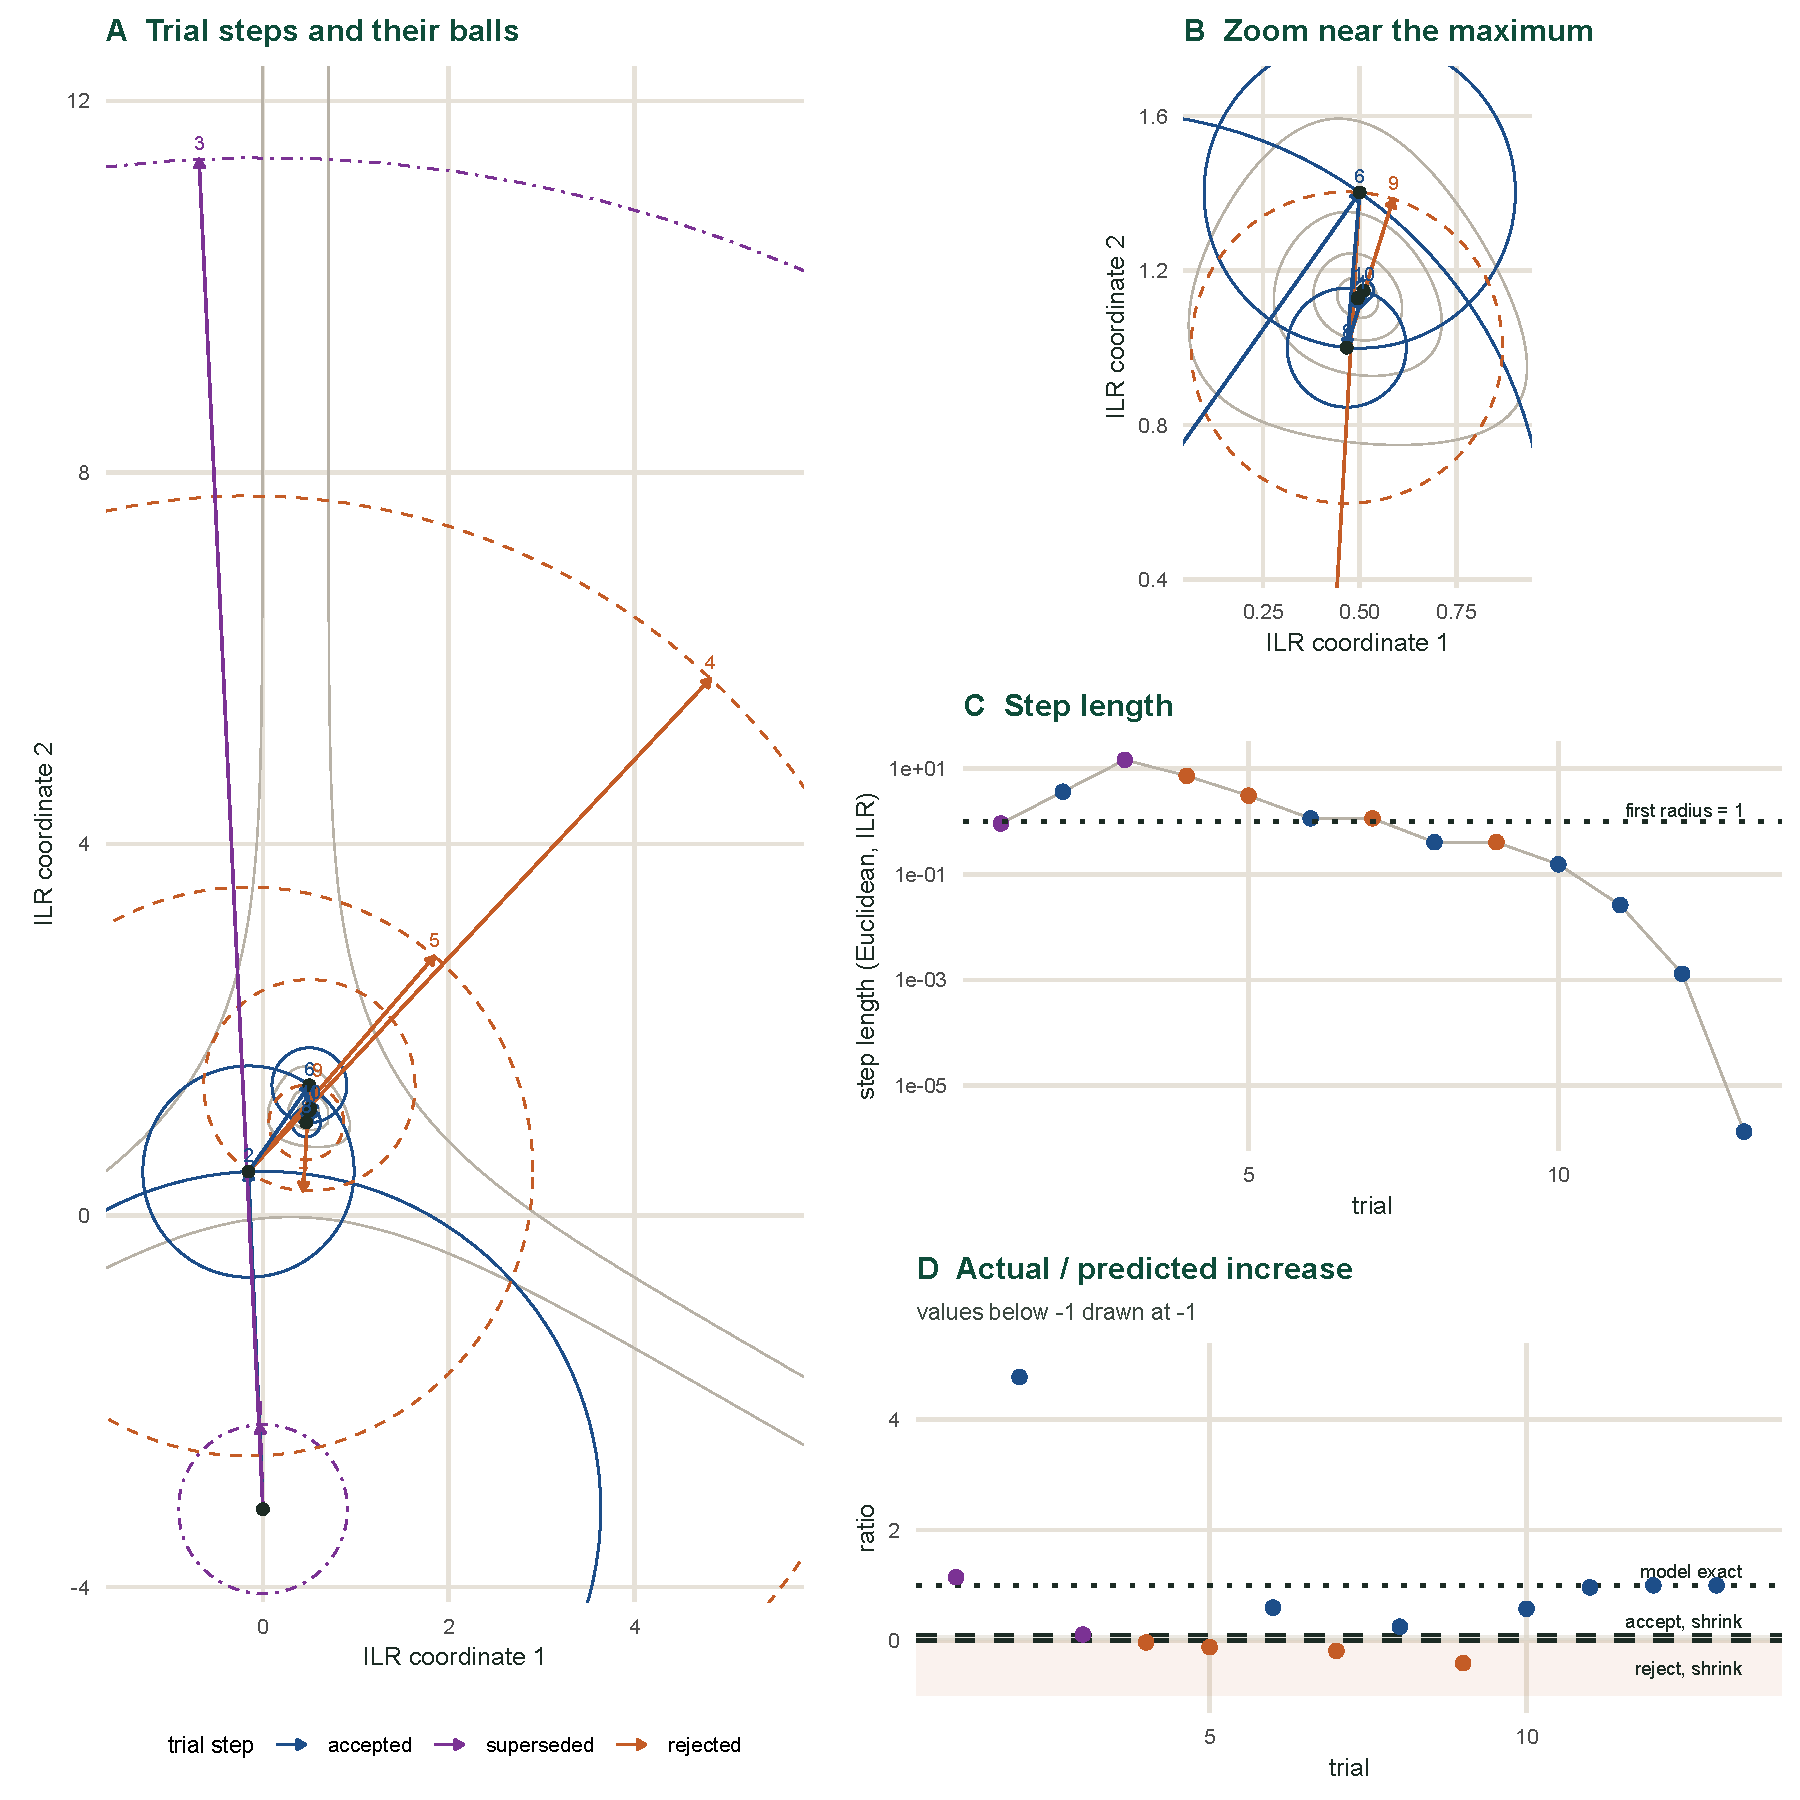
\includegraphics[width=\textwidth]{figs/fig_trust_region_steps.pdf}
  \caption{Trust-region step control of \texttt{stats::nlminb} on the single-cell profile log-likelihood
    \(\ell^{\ast}\) (\(J=3\), \(G=10\), \(n=10^{4}\) cells, cell sizes \((1,2,5)\), true fractions \((0.6,0.3,0.1)\)), started near
    the corner \(\boldsymbol{p}=(0.02,0.02,0.96)\). Every trial is an objective evaluation of \texttt{nlminb}; an iterate (black dot)
    is a point where it requested the gradient. Blue: accepted step; purple: superseded step, which increased
    \(\ell^{\ast}\) but was replaced by a longer step from the same iterate after the radius was enlarged; orange: rejected
    step, after which the radius is cut. \textbf{A}~ILR plane, grey contours of \(\ell^{\ast}\); each circle is centred on the
    iterate a trial starts from, with the length of that trial step, which equals the radius when the step lies on the
    boundary of the ball. \textbf{B}~Zoom on the last iterations. \textbf{C}~Length of every trial step (log scale): the
    radius grows by a factor 4 twice from the first radius 1, overshoots, and is then halved or interpolated down until
    a step is accepted; the last steps are full Newton steps. \textbf{D}~Ratio of the actual to the predicted
    increase; below \(10^{-4}\) the trial is rejected, between \(10^{-4}\) and \(0.1\) it is accepted with a smaller radius,
    and near 1 the quadratic model is exact. Script: \texttt{article/scripts/fig\_trust\_region\_steps.R}; the SVG source is
    \texttt{article/figs/fig\_trust\_region\_steps.svg}.}
  \label{fig:trust-region-steps}
\end{figure}

\subsubsection{Generalised least squares, Fisher scoring and iteratively reweighted least squares}
\label{app:irls}

The argument follows maximum likelihood as iteratively reweighted least squares for generalised linear models
\cite[Sects.~4.5.4--4.5.5]{agrestiFoundationsLinearGeneralized2015} \cite[Sects.~2.1--2.2]{nelderGeneralizedLinearModels1972}.

\begin{theorem}[Generalised least squares]
  \label{th:generalized-least-squares-estimate}
  Consider \(\boldsymbol{y}=\boldsymbol{X}\boldsymbol{\beta}+\boldsymbol{\varepsilon}\) with a fixed design \(\boldsymbol{X}\) of full column rank,
  \(\mathbb{E}(\boldsymbol{\varepsilon})=\boldsymbol{0}\) and \(\operatorname{Cov}(\boldsymbol{\varepsilon})=\boldsymbol{\Sigma}\), a known non-singular covariance.
  The estimate that minimises the squared Mahalanobis norm of the residuals is
  \(\hat{\boldsymbol{\beta}}^{\mathrm{GLS}}=(\boldsymbol{X}^{\top}\boldsymbol{\Omega}\boldsymbol{X})^{-1}\boldsymbol{X}^{\top}\boldsymbol{\Omega}\boldsymbol{y}\), with \(\boldsymbol{\Omega}=\boldsymbol{\Sigma}^{-1}\) and
  covariance \((\boldsymbol{X}^{\top}\boldsymbol{\Omega}\boldsymbol{X})^{-1}\).
  It is the best linear unbiased estimator of \(\boldsymbol{\beta}\), and it equals the maximum-likelihood estimate under a
  Gaussian error.
  A Cholesky factor \(\boldsymbol{\Sigma}=\boldsymbol{C}\boldsymbol{C}^{\top}\) reduces the problem to ordinary least squares on
  \(\boldsymbol{C}^{-1}\boldsymbol{y}\), which removes heteroscedasticity and residual correlation.
  Weighted least squares is the diagonal case \(\boldsymbol{\Sigma}=\operatorname{diag}(\sigma_{1}^{2},\ldots,\sigma_{G}^{2})\), a heteroscedastic
  error without correlation.
  For deconvolution, \(\boldsymbol{X}=\boldsymbol{\mu}\) and \(\boldsymbol{\beta}=\boldsymbol{p}_{\cdot i}\); the simplex constraint is imposed afterwards, or
  through the chart \eqref{eq-mapping-function}.
\end{theorem}

\begin{itemize}
  \item Newton--Raphson and \gls{fisherscoring} differ only in the curvature matrix:
        \begin{equation}
          \boldsymbol{\rho}^{(t+1)}=\boldsymbol{\rho}^{(t)}-\{\nabla^{2}_{\boldsymbol{\rho}}\ell(\boldsymbol{\rho}^{(t)})\}^{-1}\nabla_{\boldsymbol{\rho}}\ell(\boldsymbol{\rho}^{(t)}),
          \qquad
          \boldsymbol{\rho}^{(t+1)}=\boldsymbol{\rho}^{(t)}+I_{\boldsymbol{\rho}}(\boldsymbol{\rho}^{(t)})^{-1}\nabla_{\boldsymbol{\rho}}\ell(\boldsymbol{\rho}^{(t)}),
          \label{eq-newton-fisher}
        \end{equation}
        the observed Hessian for the first, the expected information
        \(I_{\boldsymbol{\rho}}=\mathbf{J}_{\psi}^{\top}I(\boldsymbol{p})\mathbf{J}_{\psi}\) of \eqref{eq-expected-fisher-p} for the second
  \item working response: write \(\boldsymbol{m}(\boldsymbol{\rho})=\boldsymbol{\mu}\boldsymbol{\psi}(\boldsymbol{\rho})\), and, at the current iterate,
        \(\boldsymbol{D}_{t}=\partial\boldsymbol{m}/\partial\boldsymbol{\rho}^{\top}=\boldsymbol{\mu}\mathbf{J}_{\psi}(\boldsymbol{\rho}^{(t)})\) and
        \(\boldsymbol{V}_{t}=\boldsymbol{\Sigma}(\boldsymbol{\psi}(\boldsymbol{\rho}^{(t)}))\); the mean part of the score is
        \(\boldsymbol{D}_{t}^{\top}\boldsymbol{V}_{t}^{-1}(\boldsymbol{y}-\boldsymbol{m}_{t})\) and that of the information is \(\boldsymbol{D}_{t}^{\top}\boldsymbol{V}_{t}^{-1}\boldsymbol{D}_{t}\), so the
        Fisher-scoring step for the mean part is
        \begin{equation}
          \boldsymbol{\rho}^{(t+1)}=(\boldsymbol{D}_{t}^{\top}\boldsymbol{V}_{t}^{-1}\boldsymbol{D}_{t})^{-1}\boldsymbol{D}_{t}^{\top}\boldsymbol{V}_{t}^{-1}\boldsymbol{z}_{t},
          \qquad
          \boldsymbol{z}_{t}=\boldsymbol{D}_{t}\boldsymbol{\rho}^{(t)}+\{\boldsymbol{y}-\boldsymbol{m}(\boldsymbol{\rho}^{(t)})\},
          \label{eq-irls}
        \end{equation}
        the generalised least-squares fit of Theorem~\ref{th:generalized-least-squares-estimate} with design \(\boldsymbol{D}_{t}\) and
        covariance \(\boldsymbol{V}_{t}\); the working response \(\boldsymbol{z}_{t}\) is the observed bulk corrected by the first-order
        expansion \(\boldsymbol{m}(\boldsymbol{\rho})\approx\boldsymbol{m}_{t}+\boldsymbol{D}_{t}(\boldsymbol{\rho}-\boldsymbol{\rho}^{(t)})\) of the mean, the counterpart of the adjusted
        dependent variable \(\eta+(y-\mu)\,\mathrm{d}\eta/\mathrm{d}\mu\) of a generalised linear model
  \item differences with a generalised linear model: the link acts on the parameter, so the design \(\boldsymbol{D}_{t}\)
        changes at each iteration, while a generalised linear model keeps \(\boldsymbol{X}\) fixed and updates diagonal weights
        \((\mathrm{d}\mu/\mathrm{d}\eta)^{2}/V(\mu)\); here the weight \(\boldsymbol{V}_{t}^{-1}\) is a full gene--gene precision
  \item at convergence, \((\boldsymbol{D}^{\top}\boldsymbol{V}^{-1}\boldsymbol{D})^{-1}\) is the mean part of the Wald covariance of \(\hat{\boldsymbol{\rho}}\), and the
        generalised hat matrix \(\boldsymbol{H}=\boldsymbol{D}(\boldsymbol{D}^{\top}\boldsymbol{V}^{-1}\boldsymbol{D})^{-1}\boldsymbol{D}^{\top}\boldsymbol{V}^{-1}\), an oblique projection, supplies the
        leverages of the \gls{hccorr}
  \item chart: an ALR chart, the multinomial logit with a reference type, has \(\boldsymbol{D}^{\mathrm{alr}}=\boldsymbol{D}\boldsymbol{A}_{r}^{-1}\) with
        \(\boldsymbol{A}_{r}=\boldsymbol{D}_{r}\mathbf{V}\) (Table~\ref{tab:charts}); a Fisher-scoring step is invariant to this linear change of
        basis, so ALR and ILR produce the same iterates in \(\boldsymbol{p}\), and the Helmert basis only fixes the
        coordinates in which \(I_{\boldsymbol{\rho}}^{-1}\) is reported
  \item full Gaussian scoring: the covariance also depends on \(\boldsymbol{\rho}\), with
        \(\boldsymbol{V}_{k}=\partial\boldsymbol{V}/\partial\rho_{k}=\sum_{j}2p_{j}(\partial p_{j}/\partial\rho_{k})\boldsymbol{\Sigma}_{j}\); the score gains
        \(\tfrac12\operatorname{tr}\{\boldsymbol{V}^{-1}\boldsymbol{V}_{k}\boldsymbol{V}^{-1}(\boldsymbol{r}\boldsymbol{r}^{\top}-\boldsymbol{V})\}\) and the information
        \(\tfrac12\operatorname{tr}(\boldsymbol{V}^{-1}\boldsymbol{V}_{k}\boldsymbol{V}^{-1}\boldsymbol{V}_{l})\), so the full step is a reweighted fit of the first and second
        moments together, \(\boldsymbol{y}\) and \(\boldsymbol{r}\boldsymbol{r}^{\top}\)
  \item analogue of a canonical link: for a canonical link the second derivative of the canonical parameter
        with respect to the linear predictor vanishes, the Hessian does not depend on \(\boldsymbol{y}\), and Newton--Raphson is
        Fisher scoring \cite[Sect.~4.5.5]{agrestiFoundationsLinearGeneralized2015} \cite[Sect.~2.2]{nelderGeneralizedLinearModels1972};
        in \eqref{eq-hessian-log-likelihood-unconstrained}, the terms that separate \(\mathbf{H}\) from \(-I(\boldsymbol{p})\) all come from the
        dependence of \(\boldsymbol{\Sigma}\) on \(\boldsymbol{p}\), so they vanish when the covariance is fixed: the barycentre freeze
        \eqref{eq-gls-barycentre}, or the single-cell model \eqref{eq:sc-model} with a common within-type covariance
        \(\boldsymbol{\Sigma}_{W,j}=\boldsymbol{\Sigma}_{W}\) and fixed scales \(c\) and \(\phi\), for which \(\boldsymbol{S}_{W}(\boldsymbol{p})=\sum_{j}p_{j}\boldsymbol{\Sigma}_{W}=\boldsymbol{\Sigma}_{W}\) on the simplex; the
        log-likelihood is then quadratic in \(\boldsymbol{p}\), \(\mathbf{H}=-\boldsymbol{\mu}^{\top}\boldsymbol{\Omega}\boldsymbol{\mu}=-I(\boldsymbol{p})\), and both methods reach the
        unconstrained generalised least-squares estimate in one step; in the population-level model a common
        covariance is not enough, since \(\boldsymbol{\Sigma}(\boldsymbol{p})=(\sum_{j}p_{j}^{2})\boldsymbol{\Sigma}\) still depends on \(\boldsymbol{p}\)
  \item in the ILR chart, the chart curvature adds \(\sum_{j}(\partial\ell/\partial p_{j})\nabla^{2}_{\boldsymbol{\rho}}p_{j}\) to the Hessian
        \eqref{eq-chain-rule-second-order}, which vanishes only at an interior maximum (Appendix~\ref{app:kkt}); even with a
        fixed covariance, the two methods then share their limit and their curvature at the limit, not their path
  \item choice (our assessment): Fisher scoring far from the maximum, because \(I_{\boldsymbol{\rho}}\) is \gls{posdef} under
        (R5) of Proposition~\ref{pr:mle-regularity} while the observed Hessian can be indefinite
        (Appendix~\ref{app:mle}), so each step is an ascent direction, and it needs no second derivative of the
        chart; Newton--Raphson near the maximum, where it converges quadratically and Fisher scoring only
        linearly, at a rate set by the residual terms; the observed Hessian is needed at the end in any case, to
        certify a local maximum; under a misspecified variance function, the quasi-score of
        Section~\ref{sec:generalized-linear-model} is solved by Fisher scoring alone
  \item precedent: Jennrich and Sampson \cite{jennrichNewtonRaphsonRelatedAlgorithms1976} fitted mean and variance components of
        unbalanced mixed analysis-of-variance models by maximum likelihood, a Gaussian model whose covariance depends on the
        parameters, as in DeCovarT; Newton--Raphson, Fisher scoring and the Hemmerle--Hartley algorithm share the form
        \(\Delta\boldsymbol{\theta}=\boldsymbol{Q}^{-1}\partial\ell/\partial\boldsymbol{\theta}\) and differ only in \(\boldsymbol{Q}\); their safeguards were
        step-halving (\(\Delta\boldsymbol{\theta},\Delta\boldsymbol{\theta}/2,\Delta\boldsymbol{\theta}/4,\ldots\) until \(\ell\) increases), a Fisher-scoring
        step whenever \(\boldsymbol{Q}\) lost positive definiteness, one scoring step to start Newton--Raphson and another whenever
        the increase in \(\ell\) exceeded 1, and partial steps up to the boundary of the variance components; on five
        problems, Newton--Raphson converged in four iterations from good starts on the fifth one, while from poor starts most
        early steps defaulted to scoring and its advantage largely vanished; the authors call the safeguards
        ``admittedly ad hoc'', and no method dominated
  \item implemented choice: Newton--Raphson with the observed Hessian inside a trust region (Remark~\ref{rem:step-size}), for
        both models; the trust region removes the reason for Fisher scoring far from the maximum, since its shifted system
        \(\lambda\mathbf{I}-\nabla^{2}\ell\) is positive definite even where \(\nabla^{2}\ell\) is not, and keeps the quadratic rate near the
        maximum; the expected information is kept for the Wald variances; in the single-cell model the mean part of the
        information scales with \(c^{2}/\phi=n\), the number of cells, while the covariance part stays of order one, so near the
        maximum the observed and expected information nearly coincide and Fisher scoring would add little
\end{itemize}

\subsubsection{Robust variants of the weighted fit}
\label{sec:robust}

\begin{itemize}
  \item DeCovarT as generalised least squares (GLS)
  \begin{itemize}
    \item for a fixed weight matrix, the Mahalanobis term of
          \eqref{eq-loglikelihood-multivariate-gaussian} is the GLS criterion
          (Theorem~\ref{th:generalized-least-squares-estimate}); weighted least squares, as in \emph{DWLS}, is
          its diagonal case \cite{tsoucasAccurateEstimationCelltype2019}
    \item \emph{DECALS} solves a constrained GLS with a covariance estimated from the bulk cohort
          \cite{caiStatisticalInferenceCelltype2024}; DeCovarT uses a known, plug-in covariance whose weight
          \(\boldsymbol{\Sigma}(\boldsymbol{p})^{-1}\) moves with the composition, plus a log-determinant term
    \item DeCovarT is therefore a GLS with a parameter-dependent variance function, fitted by the reweighted
          iteration \eqref{eq-irls} once its mean part is isolated
    \item a simpler competitor freezes the residual covariance at the barycentre \(p_{j}=1/J\),\label{app:special}
          \begin{equation}
            \operatorname{Cov}(\boldsymbol{y}_{\cdot i}\mid\boldsymbol{\mu})=\frac{1}{J^{2}}\sum_{j=1}^{J}\boldsymbol{\Sigma}_{j},
            \label{eq-gls-barycentre}
          \end{equation}
          so the fit is generalised least squares on the linear mean \eqref{eq-linear-deconvolution}, for which
          Newton--Raphson and Fisher scoring coincide (Appendix~\ref{app:irls}); weighted least squares is its diagonal
          case, with the dampened gene weights of \emph{DWLS} \cite{tsoucasAccurateEstimationCelltype2019}; interaction
          monomials \(p_{j}p_{\ell}\) (a Scheff\'e expansion) can be added to the mean on the same residual, at the cost of
          many extra parameters; the frozen weight ignores the
          cell-type-specific networks, and \emph{cellGeometry} estimates such a gene-level covariance from cross-sample
          variances \cite{lauCellGeometryUltrafastSinglecell2026}
  \end{itemize}
  \item DeCovarT is not robust in the statistical sense: the loss is quadratic in the whitened residual
        \(\boldsymbol{e}=\boldsymbol{L}^{-1}(\boldsymbol{y}-\boldsymbol{\mu}\boldsymbol{p})\), so one gene with a platform shift, or a gene expressed
        by a type missing from the reference, has unbounded influence on \(\hat{\boldsymbol{p}}\); fixed gene
        weights rescale that influence without bounding it
  \item robust rewrites, in increasing departure from the current solver
  \begin{enumerate}
    \item fixed gene weights folded into the convolution,
          \(\boldsymbol{y}^{\star}=\boldsymbol{W}^{1/2}\boldsymbol{y}\), \(\boldsymbol{\mu}^{\star}=\boldsymbol{W}^{1/2}\boldsymbol{\mu}\),
          \(\boldsymbol{\Sigma}_{j}^{\star}=\boldsymbol{W}^{1/2}\boldsymbol{\Sigma}_{j}\boldsymbol{W}^{1/2}\), as \emph{BayesPrism} does with \emph{DWLS}
          weights \cite{zhangIntegratedInferenceCellularCompositions2026}; the solver is unchanged
    \item M-estimation on gene-wise standardised residuals
          \(e_{g}=r_{g}/\{\boldsymbol{\Sigma}(\boldsymbol{p})\}_{gg}^{1/2}\): replace \(\tfrac12\sum_{g}e_{g}^{2}\) by \(\sum_{g}\varrho_{c}(e_{g})\)
          with a Huber or bisquare loss
          \cite{hampelIntroductionHuber19641992,GeneralizedLinearModels2018}, solved by iteratively
          reweighted least squares with weights
          \(w_{g}=\varrho_{c}'(e_{g})/e_{g}\), and report the sandwich variance
          \(\boldsymbol{H}^{-1}\boldsymbol{K}\boldsymbol{H}^{-1}\) (Appendix~\ref{app:mle-firth})
    \item trimmed likelihood: drop the genes with the largest contributions to
          \eqref{eq-loglikelihood-multivariate-gaussian} and refit, as least trimmed squares does for
          observations \cite{rousseeuwComputingLTSRegression2006}
    \item robust reference moments: estimate \(\boldsymbol{\Sigma}_{j}\) from cells with a high-breakdown estimator
          such as the minimum covariance determinant \cite{rousseeuwMultivariateEstimationHigh1985}, so outlier
          cells do not distort the plug-in
  \end{enumerate}
  \item caution: the Cholesky whitening mixes genes, so down-weighting one whitened coordinate does not
        down-weight one gene; gene-level weights must act on gene-wise standardised residuals
\end{itemize}

\subsubsection{Other optimisation strategies}
\label{app:optim-other}

\begin{itemize}
  \item first-order methods (gradient ascent, L-BFGS) avoid the Hessian, but for one bulk sample the
        \((J-1)\times(J-1)\) Newton system is negligible next to the \(G\times G\) factorisation of \(\boldsymbol{\Sigma}(\boldsymbol{p})\) that
        every method needs
  \item stochastic and mini-batch gradients, with adaptive step sizes, scale with the number of
        independent observations; they pay off for a joint fit over many bulk samples, as in the design model of
        Section~\ref{sec:generalized-linear-model} or a joint estimate of the \(\boldsymbol{\Sigma}_{j}\) over a cohort; sub-sampling
        genes within one sample is not equivalent, because genes are correlated observations of one draw
  \item proximal gradient and ADMM handle non-smooth penalties, such as a lasso on the precisions or on the
        design coefficients \(\boldsymbol{B}\)
  \item the expectation--maximisation algorithm fits the latent-profile formulation of Section~\ref{sec:wiener}
        \cite{dempsterMaximumLikelihoodIncomplete1977}
\end{itemize}

\subsubsection{Latent profiles: the Wiener filter and BLEND}
\label{app:wiener-blend}

\begin{itemize}
  \item latent form of DeCovarT (Section~\ref{sec:wiener}): \(\boldsymbol{x}_{\cdot j,i}\sim\mathcal{N}_{G}(\boldsymbol{\mu}_{\cdot j},\boldsymbol{\Sigma}_{j})\), independent
        across types, and \(\boldsymbol{y}_{\cdot i}\mid\boldsymbol{p}_{\cdot i},\{\boldsymbol{x}_{\cdot j,i}\}\sim\mathcal{N}_{G}(\sum_{j}p_{ji}\boldsymbol{x}_{\cdot j,i},\boldsymbol{D})\); given
        \(\boldsymbol{p}_{\cdot i}\), the posterior mean, the best linear unbiased predictor and the Wiener filter coincide,
        \(\hat{\boldsymbol{x}}_{\cdot j,i}=\boldsymbol{\mu}_{\cdot j}+p_{ji}\boldsymbol{\Sigma}_{j}\boldsymbol{W}(\boldsymbol{y}_{\cdot i}-\boldsymbol{\mu}\boldsymbol{p}_{\cdot i})\) with
        \(\boldsymbol{W}=\{\boldsymbol{\Sigma}(\boldsymbol{p}_{\cdot i})+\boldsymbol{D}\}^{-1}\), and the posterior covariance is
        \(\operatorname{Cov}(\boldsymbol{x}_{\cdot j,i},\boldsymbol{x}_{\cdot k,i}\mid\boldsymbol{y}_{\cdot i},\boldsymbol{p}_{\cdot i})=\delta_{jk}\boldsymbol{\Sigma}_{j}-p_{ji}p_{ki}\boldsymbol{\Sigma}_{j}\boldsymbol{W}\boldsymbol{\Sigma}_{k}\);
        its negative cross-type blocks record that two types compete for the same residual
  \item EM: the E-step computes these means and covariances from one Cholesky factor of
        \(\boldsymbol{\Sigma}(\boldsymbol{p})+\boldsymbol{D}\); the M-step maximises a concave quadratic in \(\boldsymbol{p}\) on the simplex,
        so each iteration increases the marginal likelihood, slowly when \(\boldsymbol{D}\) is small
        (\vignette{05-2-bayesian-wiener.html}{Wiener-filter vignette})
  \item \emph{Unico}'s Theorem~1 is the gene-wise analogue with the roles of genes and types exchanged: for gene \(g\), the
        vector across types has covariance \(\boldsymbol{\Gamma}_{g}\) (\(J\times J\)) and
        \(\hat{\boldsymbol{x}}_{g\cdot,i}=\boldsymbol{\mu}_{g\cdot}+\boldsymbol{\Gamma}_{g}\boldsymbol{p}_{\cdot i}(y_{gi}-\boldsymbol{p}_{\cdot i}^{\top}\boldsymbol{\mu}_{g\cdot})/(\boldsymbol{p}_{\cdot i}^{\top}\boldsymbol{\Gamma}_{g}\boldsymbol{p}_{\cdot i}+\tau_{g}^{2})\)
        \cite[p.~12]{chenUnicoUnifiedModelCell2025}; with one gene and a diagonal \(\boldsymbol{\Gamma}_{g}\) it is the formula above
  \item \emph{BLEND} \cite{huangBLENDProbabilisticCellular2024} also returns a profile per type and per sample, by a different
        route (Table~\ref{tab:wiener-blend})
  \begin{itemize}
    \item model (p.~8): \(\boldsymbol{q}_{\cdot i}\sim\mathrm{Dir}(\boldsymbol{\alpha})\), \(\boldsymbol{\psi}_{j,i}\sim\mathrm{Dir}(\boldsymbol{\beta}_{j})\), and the reads of sample \(i\)
          are multinomial with gene probabilities \(\sum_{j}q_{ji}\boldsymbol{\Phi}^{\mathrm{B}}_{j,i}\), where
          \(\boldsymbol{\Phi}^{\mathrm{B}}_{j,i}=\sum_{m}\psi_{j,i,m}\boldsymbol{\Phi}_{j,m}\) is a convex combination of the \(M_{j}\) observed references of type \(j\)
    \item inference (pp.~9--10): Gibbs sampling with each read's reference source as a latent label, or EM for the
          posterior mode; Dirichlet concentrations of \(0.01\), which favour sparse weights (our remark)
    \item stated limits (p.~7): gene--gene correlation is ignored, and the authors judge inference on the fractions
          inappropriate although the posterior is available
    \item our remarks: the hull restricts each sample's profile to \(M_{j}-1\) free weights, so a deviation that no reference
          shows cannot be expressed, whereas the Wiener filter shrinks continuously along \(\boldsymbol{\Sigma}_{j}\); across samples
          the hull implies
          \(\operatorname{Cov}(\boldsymbol{\Phi}^{\mathrm{B}}_{j,i})=\boldsymbol{\Phi}_{j}\operatorname{Cov}(\boldsymbol{\psi}_{j,i})\boldsymbol{\Phi}_{j}^{\top}\), a gene covariance of rank at most
          \(M_{j}-1\); a sample covariance of the \(M_{j}\) references used as \(\boldsymbol{\Sigma}_{j}\) would make the Wiener filter
          the continuous, Gaussian counterpart of that hull
  \end{itemize}
\end{itemize}

\begin{table}[ht]
  \centering
  \small
  \caption{Sample-specific profiles in DeCovarT's latent form (Wiener filter) and in \emph{BLEND}.}
  \label{tab:wiener-blend}
  \begin{tabularx}{\textwidth}{@{}lYY@{}}
    \toprule
     & DeCovarT, Wiener filter & \emph{BLEND} \\
    \midrule
    Likelihood scale & Gaussian on a linear scale, diagonal residual \(\boldsymbol{D}\) & multinomial read counts \\
    Reference(s) & one mean \(\boldsymbol{\mu}_{\cdot j}\) and covariance \(\boldsymbol{\Sigma}_{j}\) per type & \(M_{j}\) observed references per type, each a distribution over genes \\
    Per-sample profile & \(\boldsymbol{\mu}_{\cdot j}+p_{ji}\boldsymbol{\Sigma}_{j}\boldsymbol{W}(\boldsymbol{y}_{\cdot i}-\boldsymbol{\mu}\boldsymbol{p}_{\cdot i})\), any vector in \(\mathbb{R}^{G}\) & \(\sum_{m}\psi_{j,i,m}\boldsymbol{\Phi}_{j,m}\), in the convex hull of the references \\
    Gene--gene covariance & full \(\boldsymbol{\Sigma}_{j}\), from a sparse precision & none stated; rank at most \(M_{j}-1\), implied by the hull (our remark) \\
    Inference & closed form given \(\boldsymbol{p}_{\cdot i}\); EM or Newton for \(\boldsymbol{p}_{\cdot i}\) & Gibbs sampling, or EM for the posterior mode \\
    Uncertainty on \(\boldsymbol{p}_{\cdot i}\) & Wald or bootstrap intervals; the profile posterior plugs in \(\hat{\boldsymbol{p}}_{\cdot i}\) & posterior available, not used for inference by the authors \\
    Cell size & cell fractions when the reference keeps \(S_{j}\) & RNA fractions, divided by \(S_{j}\) afterwards \\
    \bottomrule
  \end{tabularx}
\end{table}

\subsubsection{Structured factorisations of the mixture covariance}
\label{app:optim-structured}

\begin{itemize}
  \item cost: every evaluation of the log-likelihood, score or Hessian assembles the mixture covariance,
        \(\boldsymbol{\Sigma}(\boldsymbol{p})=\sum_{j}p_{j}^{2}\boldsymbol{\Sigma}_{j}\) or \(\boldsymbol{S}_{W}(\boldsymbol{p})=\sum_{j}p_{j}\boldsymbol{\Sigma}_{W,j}\), in
        \(O(JG^{2})\), factorises it by a dense Cholesky decomposition in \(O(G^{3})\) \cite{golubMatrixComputations2013}, and
        solves against the \(J\) matrices \(\boldsymbol{\Sigma}_{j}\) for the traces of the score and Hessian, in \(O(JG^{3})\); the
        package factorises once per trial composition and shares the factor between the three evaluations
  \item sparse precisions do not help directly: \(\boldsymbol{\Sigma}_{j}=\boldsymbol{\Omega}_{j}^{-1}\) is in general dense even when
        \(\boldsymbol{\Omega}_{j}\) is sparse, and a weighted sum of covariances has no sparse precision
  \item three structures survive the mixture, provided every cell type shares them
  \begin{itemize}
    \item block-diagonal: gene modules disconnected in every type give block-diagonal \(\boldsymbol{\Sigma}_{j}\) with the same
          blocks, hence a block-diagonal mixture, factorised block by block in \(\sum_{b}O(G_{b}^{3})\), about \(B^{2}\) times
          cheaper for \(B\) equal blocks
    \item banded or sparse: a common bandwidth \(b\) gives a banded mixture, factorised in \(O(Gb^{2})\); a common sparsity
          pattern is factorised with a fill-reducing ordering computed once and reused at every composition
          \cite{chenAlgorithm887CHOLMOD2008}
    \item diagonal plus low rank with shared loadings: \(\boldsymbol{\Sigma}_{j}=\boldsymbol{D}_{j}+\boldsymbol{U}\boldsymbol{C}_{j}\boldsymbol{U}^{\top}\) gives
          \(\boldsymbol{D}(\boldsymbol{p})+\boldsymbol{U}\boldsymbol{C}(\boldsymbol{p})\boldsymbol{U}^{\top}\), solved by the Woodbury identity and its determinant by the
          matrix-determinant lemma, in \(O(Gr^{2})\) for rank \(r\) \cite{hagerUpdatingInverseMatrix1989}
  \end{itemize}
  \item no statistical effect: each route computes the same log-likelihood, score and Hessian up to round-off, so the
        estimate, its intervals and the benchmark scores do not change; only run time and memory do
  \item caveats: the structure must hold exactly and be declared, never inferred from near-zero entries, because a small
        cross-block covariance makes the block route wrong rather than approximate; adding cell types adds gene--gene
        correlations, so a pattern shared by every type is the exception, and the package keeps the dense Cholesky
  \item status: block, band, sparse and diagonal-plus-low-rank backends are in
        \texttt{scripts/experimental/covariance\_backends.R}, outside the package; the supplementary S2 script checks each
        against the dense Cholesky and times it against \(G\) and sparsity
        \todo{Run the S2 script and report time and memory against \(G\) and sparsity.}
\end{itemize}

\subsection{Maximum-likelihood properties and confidence intervals}
\label{app:mle}

Proofs and simulations in the \vignette{01-2-population-inference.html}{population inference vignette}.

\subsubsection{Existence, uniqueness and identifiability}

\begin{itemize}
  \item existence: with symmetric positive-definite \(\boldsymbol{\Sigma}_{j}\), \(\boldsymbol{\Sigma}(\boldsymbol{p})\) is positive definite
        on the closed simplex, so the log-likelihood is continuous on a compact set and attains its supremum,
        possibly on a face
  \item non-uniqueness: the model is heteroscedastic; with \(\boldsymbol{\Sigma}_{1}=\boldsymbol{\Sigma}_{2}=\mathbf{I}_{3}\),
        \(\boldsymbol{\mu}_{\cdot1}=(2,1,1)^{\top}\), \(\boldsymbol{\mu}_{\cdot2}=(1,2,6/5)^{\top}\) and \(\boldsymbol{y}=\boldsymbol{\mu}(1/2,1/2)^{\top}\), the
        Hessian \eqref{eq-hessian-log-likelihood-unconstrained} at \(\boldsymbol{p}=(1/5,3/10)\) has eigenvalues of about
        \(-654.5\) and \(+53.9\); the log-likelihood is therefore not concave, in \(\boldsymbol{p}\) or in the ILR
        chart, and a converged solver certifies a local maximum only
  \item a single bulk profile provides no replication of its own composition, so every asymptotic
        statement below is taken in the number of replicate samples sharing one composition or, for the
        single-cell model \eqref{eq:sc-model}, in the number of cells (Appendix~\ref{app:mle-regularity})
  \item population uniqueness: the expected log-likelihood is maximised only at the true composition under
        identifiability, because the gap is a Kullback--Leibler divergence \cite{vaartAsymptoticStatistics2000}
  \item ILR versus \emph{MEAD}: \emph{MEAD} truncates or softplus-transforms its estimate, which is inconsistent for a
        finite softplus constant \cite{xieStatisticalInferenceCell2026}; the softmax chart gives exact positivity with
        no tuning, and a true zero sits at infinity in ILR coordinates
\end{itemize}

\subsubsection{Regularity conditions and asymptotic regimes}
\label{app:mle-regularity}

Intervals in this appendix follow the generalised-linear-model treatment of likelihood inference
\cite[Sects.~4.2--4.3]{agrestiFoundationsLinearGeneralized2015}; the asymptotic theory is that of
\cite[Ch.~9]{coxTheoreticalStatistics1979}.

\begin{proposition}[Large-sample normality and the three first-order tests]
  \label{pr:mle-regularity}
  Let \(\boldsymbol{y}_{\cdot1},\ldots,\boldsymbol{y}_{\cdot N}\) be independent bulk profiles of \(N\) biological samples that share
  one composition \(\boldsymbol{p}_{0}\), and write \(\boldsymbol{\rho}_{0}=\mathbf{V}^{\top}\log\boldsymbol{p}_{0}\).
  Assume that
  \begin{enumerate}
    \item[(R1)] the composition is identifiable: distinct compositions give distinct laws (Appendix~\ref{app:mle});
    \item[(R2)] the truth is an interior point: \(\boldsymbol{p}_{0}\) lies in the open simplex, so \(\boldsymbol{\rho}_{0}\) is a finite
          point of the open set \(\mathbb{R}^{J-1}\);
    \item[(R3)] the number of free parameters \(J-1\), and the number of genes \(G\), stay fixed while
          \(N\to\infty\);
    \item[(R4)] the log-density is three times continuously differentiable in \(\boldsymbol{\rho}\) near \(\boldsymbol{\rho}_{0}\), with third
          derivatives bounded by an integrable function;
    \item[(R5)] the per-sample Fisher information \(I_{\boldsymbol{\rho}}(\boldsymbol{\rho}_{0})\) is finite and \gls{posdef};
    \item[(R6)] the support of the law does not depend on \(\boldsymbol{\rho}\), and differentiation and integration
          can be interchanged.
  \end{enumerate}
  Then, with probability tending to one, the likelihood equation has a consistent root, and
  \(\sqrt{N}(\hat{\boldsymbol{\rho}}-\boldsymbol{\rho}_{0})\rightsquigarrow\mathcal{N}_{J-1}(\boldsymbol{0},I_{\boldsymbol{\rho}}(\boldsymbol{\rho}_{0})^{-1})\).
  For a null hypothesis that fixes \(k\) smooth functions of \(\boldsymbol{\rho}\), the Wald, likelihood-ratio and
  score statistics of Appendix~\ref{app:mle-tests} all converge to \(\chi^{2}_{k}\), and they differ by
  \(o_{P}(1)\) \cite[Sects.~9.2--9.3]{coxTheoreticalStatistics1979}.
\end{proposition}

\begin{remark}[The same theorem in Keener, and the Godambe generalisation]
  \label{rem:keener-godambe}
  \begin{itemize}
    \item Theorem~9.14 of Keener's \emph{Theoretical Statistics} \cite{keenerEstimatingEquationsMaximum2010} states the result of
          Proposition~\ref{pr:mle-regularity} for independent and identically distributed observations: under regularity
          conditions of the same kind, \(\sqrt{N}(\hat{\boldsymbol{\theta}}_{N}-\boldsymbol{\theta}^{\ast})\rightsquigarrow\mathcal{N}(\boldsymbol{0},I(\boldsymbol{\theta}^{\ast})^{-1})\),
          with \(I\) the Fisher information of one observation, so the estimate is asymptotically efficient and Wald intervals
          follow from the diagonal of \(I(\hat{\boldsymbol{\theta}})^{-1}/N\); \emph{RNA-Sieve} invokes it for its proportions and its
          scale \(n\), treating the genes of one bulk as the replicates
          \cite{erdmann-phamLikelihoodbasedDeconvolutionBulk2021}
    \item under misspecification, when the data law \(Q\) lies outside the model family, the maximiser converges to the
          Kullback--Leibler projection \(\boldsymbol{\theta}_{p}\) of \(Q\) on the family, and its covariance is the inverse Godambe
          information \(\boldsymbol{H}^{-1}\boldsymbol{B}\boldsymbol{H}^{-\top}/N\), with \(\boldsymbol{H}\) the expected Hessian and \(\boldsymbol{B}\) the variance of the
          score of one observation \cite{godambeOptimumPropertyRegular1960}; it reduces to \(I^{-1}/N\) when the model is right, since then \(\boldsymbol{B}=-\boldsymbol{H}=I\)
    \item the Godambe interval covers \(\boldsymbol{\theta}_{p}\), not the truth: \emph{RNA-Sieve} argues that \(\boldsymbol{\theta}_{p}\approx\boldsymbol{\theta}^{\ast}\)
          when a protocol shift rescales the reference means globally rather than changing their distribution
    \item for one bulk, the genes are the observations of this argument only if they are independent, which is
          \emph{RNA-Sieve}'s assumption; DeCovarT models their dependence, so its replicate unit is the bulk sample, or the
          cell in the small-dispersion regime below
    \item in the benchmarks, the per-gene scores and averaged Hessian of \emph{RNA-Sieve} give
          \(\boldsymbol{B}^{-1}/G\) (empirical Fisher) and \(\boldsymbol{H}^{-1}\boldsymbol{B}\boldsymbol{H}^{-\top}/G\) (Godambe) in the coordinates
          \((\alpha_{1},\ldots,\alpha_{K-1},n)\), with \(\alpha_{K}=1-\sum_{k<K}\alpha_{k}\), so the variance of \(\alpha_{K}\) is
          \(\mathbf{1}^{\top}\boldsymbol{V}\mathbf{1}\) over the first \(K-1\) coordinates (Section~\ref{sec:hd})
  \end{itemize}
\end{remark}

\begin{itemize}
  \item the Gaussian convolution meets (R4) and (R6) on the open simplex, because
        \(\boldsymbol{\Sigma}(\boldsymbol{p})\) is positive definite on the closed simplex; (R5) fails when signature
        columns are collinear and the covariances do not separate the types
  \item (R2) fails when a type is absent: the limit is then a chi-bar-square mixture
        (Appendix~\ref{app:mle-boundary})
  \item (R3) sets the direction of the limit: the replication unit is the biological sample \(i\), not the
        gene; the \(G\) genes are correlated by construction, and a design that adds one composition for
        each new sample adds parameters as fast as observations, so no single composition gains
        information \cite[p.~81]{coxTheoreticalStatistics1979}
  \item small-dispersion regime: a single bulk sample (\(N=1\)) still has an asymptotic direction under
        \eqref{eq:sc-model}; with \(\tilde{\boldsymbol{y}}_{\cdot i}=\boldsymbol{y}_{\cdot i}/c_{i}\), the law is
        \(\mathcal{N}_{G}(\tilde{\boldsymbol{\mu}}\boldsymbol{p}_{\cdot i},\,n_{i}^{-1}\boldsymbol{S}_{W}(\boldsymbol{p}_{\cdot i}))\), so the number of cells
        \(n_{i}\) plays the role of the index parameter \(\lambda\) of a dispersion model
  \begin{itemize}
    \item for one observation of a dispersion model, J{\o}rgensen proves consistency,
          \(\lambda^{1/2}(\hat{\boldsymbol{\beta}}-\boldsymbol{\beta}_{0})\rightsquigarrow\mathcal{N}(\boldsymbol{0},i(\boldsymbol{\beta}_{0})^{-1})\), and \(\chi^{2}\) limits
          for deviance differences as \(\lambda\to\infty\) with the sample size fixed, under conditions that
          mirror (R2), (R4) and (R5): an open parameter set, a full-rank local design matrix and a
          positive-definite information \cite[Theorems~4.1--4.3]{jørgensenSmallDispersionAsymptotics1987};
          large expected cell counts in contingency tables are the classical special case
    \item our remark: \eqref{eq:sc-model} is not exactly a dispersion model, because the term
          \(-\tfrac12\log\det\boldsymbol{S}_{W}(\boldsymbol{p})\) is not multiplied by \(n_{i}\); it is \(O(1)\) against the
          \(O(n_{i})\) Mahalanobis term, so the information is dominated by its mean part
          \(n_{i}\mathbf{J}_{\psi}^{\top}\tilde{\boldsymbol{\mu}}^{\top}\boldsymbol{S}_{W}^{-1}\tilde{\boldsymbol{\mu}}\mathbf{J}_{\psi}\) and the quasi-score of
          Section~\ref{sec:generalized-linear-model} becomes efficient in this limit; the proof is to be written
    \item the limit needs every type count \(m_{ji}=n_{i}p_{ji}\) to grow, not only \(n_{i}\): the Gaussian law of
          the bulk is itself a central-limit approximation over the cells of each type, so a rare type
          with few cells breaks it first
    \item with the dispersion unknown, J{\o}rgensen estimates it by the deviance divided by its degrees of
          freedom \cite[Sect.~4.5]{jørgensenSmallDispersionAsymptotics1987}; here this is the Pearson estimate
          \(\hat\phi\) on \(G-J\) degrees of freedom, so \(G\) must exceed \(J\) by a margin and \(t\) or \(F\)
          quantiles replace normal and \(\chi^{2}\) ones when \(G-J\) is small
    \item the reference moments \((\tilde{\boldsymbol{\mu}},\boldsymbol{\Sigma}_{W,j})\) are estimated from \(C_{j}\) cells; their error does
          not shrink with \(n_{i}\) and dominates once \(n_{i}\gg C_{j}\), which the reference bootstrap
          (Appendix~\ref{app:mle-boundary}) propagates
    \item the population-level covariance \(\sum_{j}p_{j}^{2}\boldsymbol{\Sigma}_{j}\) has no index parameter, so for it only the
          replicate limit of Proposition~\ref{pr:mle-regularity} is available
  \end{itemize}
\end{itemize}

\subsubsection{Local geometry of the log-likelihood}
\label{app:mle-geometry}

\begin{itemize}
  \item every first-order interval reads the curvature at the estimate: near \(\hat{\boldsymbol{\rho}}\),
        \(\ell(\boldsymbol{\rho})-\ell(\hat{\boldsymbol{\rho}})\approx-\tfrac12(\boldsymbol{\rho}-\hat{\boldsymbol{\rho}})^{\top}\boldsymbol{j}(\hat{\boldsymbol{\rho}})(\boldsymbol{\rho}-\hat{\boldsymbol{\rho}})\), with
        \(\boldsymbol{j}=-\nabla^{2}_{\boldsymbol{\rho}}\ell\) the observed information; a scalar Wald half-width is
        \(z_{1-\alpha/2}\,\boldsymbol{j}^{-1/2}\), so a sharp peak gives a narrow interval and a plateau a wide one;
        a ridge, as along the contrast of two collinear signatures, gives an elongated ellipse
  \item anisotropy is read from the \gls{condnum} \(\kappa=\lambda_{\max}/\lambda_{\min}\) of the Hessian at the returned
        estimate: Wald half-widths along its eigenvectors scale as \(\lambda^{-1/2}\), so a large \(\kappa\) signals an
        elongated peak, and a \(\lambda_{\min}\) close to zero a plateau or a ridge along the corresponding eigenvector,
        where the interval is wide and the inversion of \(\boldsymbol{j}\) loses accuracy; \(\kappa\) alone misses a flat but
        round peak: in the archived run of the covariance-driven scenario (\(N=50\)), \(\kappa\) of the ILR information
        fell from \(6.8\) to \(1.7\) as the overlap grew, because both eigenvalues shrank
        (\vignette{R2-covariance-driven.html\#sec-hybrid-findings}{covariance-driven vignette}), so
        \(\lambda_{\min}\) is read together with \(\kappa\)
  \item Gaussian response, identity link, known covariance: \(\ell\) is exactly quadratic in the coefficients,
        the Wald, likelihood-ratio and score statistics are equal, their \(\chi^{2}\) law is exact, and the
        symmetric interval is exact \cite[Sect.~4.3]{agrestiFoundationsLinearGeneralized2015}
  \item DeCovarT departs from that case in three ways
  \begin{itemize}
    \item the covariance \(\boldsymbol{\Sigma}(\boldsymbol{p})\) depends on the parameter, so \(\ell\) is not quadratic even in
          \(\boldsymbol{p}\), where the mean is linear
    \item the chart is nonlinear: the mean \(\boldsymbol{\mu}\boldsymbol{\psi}(\boldsymbol{\rho})\) is not linear in \(\boldsymbol{\rho}\)
    \item near a face, \(p_{j}\to0\) sends \(\rho\) to infinity and \(\ell\) flattens; with few replicates, an
          unbalanced composition or overlapping types, the profile is skewed and the plateau is wide; the
          ILR slices of the covariance-driven scenario show these ridges
          (\vignette{R2-covariance-driven.html\#sec-hybrid-findings}{covariance-driven vignette})
  \end{itemize}
  \item diagnostic: compare the Wald, score and likelihood-ratio intervals for the same estimate; plot
        the signed root \(r(\psi)\) of Appendix~\ref{app:mle-inversion} against the Wald pivot
        \((\hat\psi-\psi)/\mathrm{SE}\): the two coincide when \(\ell\) is quadratic, and a curved \(r(\psi)\) or a
        large gap between the three intervals flags a non-Gaussian geometry; ratios of the three
        statistics also detect the Hauck--Donner effect \cite{yeeHauckDonnerEffectWald2022}
\end{itemize}

\subsubsection{Wald, likelihood-ratio and score statistics}
\label{app:mle-tests}
\label{app:mle-intervals}

\begin{itemize}
  \item partition \(\boldsymbol{\theta}=(\boldsymbol{\psi},\boldsymbol{\lambda})\) into \(k\) parameters of interest and nuisance parameters, test
        \(H_{0}:\boldsymbol{\psi}=\boldsymbol{\psi}_{0}\), and write \(\tilde{\boldsymbol{\theta}}_{0}=(\boldsymbol{\psi}_{0},\hat{\boldsymbol{\lambda}}_{\boldsymbol{\psi}_{0}})\) for the restricted
        estimate and \(I^{\psi\psi}\) for the \(\boldsymbol{\psi}\) block of \(I^{-1}\)
        \cite[Sect.~9.3]{coxTheoreticalStatistics1979} \cite[Sect.~4.3]{agrestiFoundationsLinearGeneralized2015}:
        \begin{equation}
          \begin{aligned}
            W&=(\hat{\boldsymbol{\psi}}-\boldsymbol{\psi}_{0})^{\top}\{I^{\psi\psi}(\hat{\boldsymbol{\theta}})\}^{-1}(\hat{\boldsymbol{\psi}}-\boldsymbol{\psi}_{0}),
            \qquad
            D=2\{\ell(\hat{\boldsymbol{\theta}})-\ell(\tilde{\boldsymbol{\theta}}_{0})\},\\
            S&=\boldsymbol{U}_{\psi}(\tilde{\boldsymbol{\theta}}_{0})^{\top}I^{\psi\psi}(\tilde{\boldsymbol{\theta}}_{0})\boldsymbol{U}_{\psi}(\tilde{\boldsymbol{\theta}}_{0})
          \end{aligned}
          \label{eq-three-tests}
        \end{equation}
  \item Wald: needs only the unrestricted fit; uses the curvature at \(\hat{\boldsymbol{\theta}}\); with the delta method
        \eqref{eq-delta-method-p}, \(\hat p_{j}\pm z_{1-\alpha/2}\mathrm{SE}_{j}\) is symmetric and can leave \([0,1]\)
        for a rare type \cite{oehlertNoteDeltaMethod1992}
  \item likelihood ratio: needs both fits; invariant to any smooth reparametrisation of \(\boldsymbol{\psi}\); tests
        any nested hypothesis, including \(k\) linear constraints \(\boldsymbol{C}\boldsymbol{p}=\boldsymbol{d}\) with \(D\rightsquigarrow\chi^{2}_{k}\); in a
        lineage-aware fit (Section~\ref{sec:lineage}), the hypothesis that two child lines occur in the
        ratio \(w_{0}\) measured in their parental line is
        \(p_{c_{1}}-w_{0}(p_{c_{1}}+p_{c_{2}})=0\), one linear constraint; the restricted set is still a polytope,
        but the constraint is not linear in \(\boldsymbol{\rho}\), so the restricted fit is done in \(\boldsymbol{p}\)
  \item score: needs only the restricted fit and uses the slope of \(\ell\) at the null; Rao's score test
        and the Lagrange-multiplier test are the same statistic, since the multiplier of \(\boldsymbol{\psi}=\boldsymbol{\psi}_{0}\) at
        the restricted maximum equals \(\boldsymbol{U}_{\psi}(\tilde{\boldsymbol{\theta}}_{0})\); written in \(\boldsymbol{p}\) coordinates it is
        defined on a face, where Wald is not
  \item the three are asymptotically equivalent under Proposition~\ref{pr:mle-regularity}
        \cite[Sect.~9.3]{coxTheoreticalStatistics1979}, and they disagree exactly when the geometry of
        Appendix~\ref{app:mle-geometry} is not quadratic
  \item link with the stopping rule of the Marquardt--Levenberg solver: the relative distance to the
        maximum is \(m^{-1}\boldsymbol{U}(\boldsymbol{\theta}_{k})^{\top}\boldsymbol{G}(\boldsymbol{\theta}_{k})^{-1}\boldsymbol{U}(\boldsymbol{\theta}_{k})\), a score statistic for the null
        ``the iterate \(\boldsymbol{\theta}_{k}\) is the maximiser'' divided by the number of parameters \(m\), with
        \(\boldsymbol{G}\) an estimate of the score variance (outer products of individual scores in the robust-variance
        scoring algorithm, the Hessian in \texttt{marqLevAlg}); Commenges et al.\ note that inverting
        \(\boldsymbol{U}^{\top}\boldsymbol{G}^{-1}\boldsymbol{U}\le\chi^{2}_{m,1-\alpha}\) gives a confidence region
        \cite[pp.~10 and 13]{commengesNewtonLikeAlgorithmLikelihood2006}; its null is a statement about the
        iterate, so it certifies convergence and tests nothing about \(\boldsymbol{p}\)
\end{itemize}

\subsubsection{Confidence intervals by test inversion}
\label{app:mle-inversion}

\begin{itemize}
  \item a \((1-\alpha)\) confidence set is the set of null values that a level-\(\alpha\) test does not reject,
        \(\{\psi_{0}:T(\psi_{0})\le\chi^{2}_{1,1-\alpha}\}\) for each statistic \eqref{eq-three-tests}
        \cite[Sect.~4.3]{agrestiFoundationsLinearGeneralized2015}
  \item Wald: the information is evaluated once, at \(\hat\psi\), so the set is the symmetric interval
        \(\hat\psi\pm z_{1-\alpha/2}\mathrm{SE}(\hat\psi)\)
  \item score: the information is re-evaluated at each candidate \(\psi_{0}\), so the interval is asymmetric;
        for a binomial proportion it is the Wilson interval \cite{wilsonProbableInferenceLaw1927}
  \item likelihood ratio: \(D(\psi_{0})\) is zero at \(\hat\psi\) and grows on both sides, so
        \(\{\psi_{0}:D(\psi_{0})\le\chi^{2}_{1,1-\alpha}\}\) has a lower and an upper endpoint, where the profile deviance
        crosses the cut-off on each side of \(\hat\psi\); the \(\chi^{2}_{1}\) test is two-sided because it squares the
        signed likelihood root
        \(r(\psi_{0})=\operatorname{sign}(\hat\psi-\psi_{0})\sqrt{D(\psi_{0})}\rightsquigarrow\mathcal{N}(0,1)\); the lower limit solves
        \(r(\psi_{L})=z_{1-\alpha/2}\) and the upper limit \(r(\psi_{U})=-z_{1-\alpha/2}\), and \(z_{1-\alpha}\) gives one-sided
        limits; if \(D\) stays below the cut-off up to the face \(p_{j}=0\), the lower limit is \(0\)
  \item several parameters: the joint region \(\{\boldsymbol{\psi}_{0}:D(\boldsymbol{\psi}_{0})\le\chi^{2}_{k,1-\alpha}\}\), with the remaining
        proportions and the scales profiled out as nuisance parameters, has simultaneous coverage
  \item software: \texttt{confint\_profile\_decovart()} for DeCovarT; for generalised linear models,
        \texttt{stats::confint()} inverts the signed root of the profile, and \texttt{ProfileLikelihood} plots
        normalised profiles and likelihood support intervals; the higher-order \texttt{likelihoodAsy}
        (\(r\) and \(r^{\ast}\) for any scalar function of the parameters, given a log-likelihood and a data
        simulator) applies to DeCovarT, whereas \texttt{cond} is restricted to logistic and log-linear models
  \item back-transformation: Agresti forms the interval on the scale of the linear predictor and maps the
        endpoints by the inverse link, instead of applying the delta method to the fitted mean
        \cite[Sect.~4.2.5]{agrestiFoundationsLinearGeneralized2015}; a smooth, monotone map preserves quantiles,
        so for \(J=2\) the interval \(\psi(\hat\rho\pm z\,\mathrm{SE})\) keeps the coverage of the interval for \(\rho\) and stays
        inside \((0,1)\); for \(J>2\) the bijection \(\boldsymbol{\psi}\) maps joint regions exactly,
        \(\Pr(\boldsymbol{\rho}\in R)=\Pr\{\boldsymbol{p}\in\boldsymbol{\psi}(R)\}\), and marginal intervals for \(p_{j}\) are quantiles of
        \(\boldsymbol{\psi}(\boldsymbol{\rho}^{(b)})\) with \(\boldsymbol{\rho}^{(b)}\sim\mathcal{N}(\hat{\boldsymbol{\rho}},I_{\boldsymbol{\rho}}^{-1})\)
  \item choice of chart: the free softmax of \(J\) scores is not identifiable and its information is singular; the
        multinomial logit with a reference type is the ALR chart, a linear transform of the ILR chart, so both
        give the same estimate, the same likelihood ratio and the same delta-method covariance
        (Appendix~\ref{app:chart-derivatives}); a component-wise logit interval adds a second delta method on
        top of the first; the ILR back-transformation is therefore kept, for its numerical invariance
  \item the Wald interval remains the weakest of the three: it depends on nonlinear changes of chart
        (\(\boldsymbol{p}\), log-ratio or logit coordinates give different intervals), it is undefined on a face, and its
        symmetry presumes a quadratic log-likelihood
  \item[] \todo[inline]{Planned: intervals from the generalised-linear-model view of DeCovarT.
        Compute the \(1-\alpha/2\) and \(\alpha/2\) quantiles in ILR coordinates, where the
        quasi-score \(\boldsymbol{D}^{\top}\boldsymbol{V}^{-1}(\boldsymbol{y}-\boldsymbol{m})=\boldsymbol{0}\)
        has information \(\boldsymbol{D}^{\top}\boldsymbol{V}^{-1}\boldsymbol{D}\) (Section~\ref{sec:generalized-linear-model}),
        then map both bounds back to the simplex. Compare their coverage with the Wald interval on \(\boldsymbol{p}\), which
        can exceed the unit simplex for highly unbalanced mixtures, and with the ILR interval, which cannot
        (Appendix~\ref{app:mle-tests}).}
\end{itemize}

\subsubsection{Nuisance scales: profile likelihood and orthogonality}
\label{app:mle-nuisance}

\begin{itemize}
  \item in \eqref{eq:sc-model} the scales \(\boldsymbol{\eta}=(\log c,\log\phi)\) are technical nuisance parameters; the profile
        log-likelihood is \(\ell^{\ast}(\boldsymbol{\rho})=\ell(\boldsymbol{\rho},\hat{\boldsymbol{\eta}}(\boldsymbol{\rho}))\)
  \item by the \gls{envelope}, \(\nabla\ell^{\ast}(\boldsymbol{\rho})=\nabla_{\boldsymbol{\rho}}\ell(\boldsymbol{\rho},\boldsymbol{\eta})\rvert_{\boldsymbol{\eta}=\hat{\boldsymbol{\eta}}(\boldsymbol{\rho})}\): the profile score
        needs no derivative of \(\hat{\boldsymbol{\eta}}(\boldsymbol{\rho})\), which is how the profile score of
        Appendix~\ref{sec:sc-newton} is obtained; differentiating once more gives the Schur complement
        \(-\nabla^{2}\ell^{\ast}=\boldsymbol{j}_{\rho\rho}-\boldsymbol{j}_{\rho\eta}\boldsymbol{j}_{\eta\eta}^{-1}\boldsymbol{j}_{\eta\rho}\), so profile and joint Wald intervals agree
  \item \gls{orthogonality}: when \(I_{\rho\eta}=\boldsymbol{0}\), the information is block diagonal, \(\hat{\boldsymbol{\rho}}\) and \(\hat{\boldsymbol{\eta}}\) are
        asymptotically independent, the standard error of \(\hat{\boldsymbol{\rho}}\) is the same whether \(\boldsymbol{\eta}\) is known or estimated,
        and \(\hat{\boldsymbol{\eta}}_{\psi}\) changes only by \(O_{P}(N^{-1})\) with \(\psi\) \cite[Sect.~2.2]{coxParameterOrthogonalityApproximate1987};
        in a generalised linear model the dispersion is orthogonal to the mean parameters
  \item in \eqref{eq:sc-model}, \(I_{c\phi}=0\) but \(I_{p_{j}c}\neq0\) and \(I_{p_{j}\phi}\neq0\) (Appendix~\ref{sec:sc-newton}): the
        composition is not orthogonal to the scales, and estimating them widens the intervals through the
        Schur complement; a scalar interest parameter can always be made orthogonal to the nuisance by
        solving a system of partial differential equations, a vector one in general cannot
        \cite[Sect.~2.3]{coxParameterOrthogonalityApproximate1987}
  \item with orthogonal nuisance parameters, the Cox--Reid adjusted profile log-likelihood
        \(\ell^{\ast}(\psi)-\tfrac12\log\det\boldsymbol{j}_{\eta\eta}(\psi,\hat{\boldsymbol{\eta}}_{\psi})\) corrects the profile for the estimation of
        \(\boldsymbol{\eta}\), as restricted maximum likelihood does for a variance
        \cite{coxParameterOrthogonalityApproximate1987}
  \item the same block structure of the expected information is derived for every alignment strategy in the
        \vignette{02-1-single-cell-generative-optimisation.html\#sec-compound}{single-cell generative and optimisation vignette}
\end{itemize}

\subsubsection{Higher-order and finite-sample corrections}
\label{app:mle-firth}

\begin{itemize}
  \item first-order errors: \(r\sim\mathcal{N}(0,1)+O(n^{-1/2})\) and \(D\sim\chi^{2}_{k}+O(n^{-1})\), where \(n\) is the sample
        size or any parameter that controls the convergence to the asymptotic limit
        \cite{canoneroHigherorderAsymptoticCorrections2023}, here the number of replicates \(N\) or the number of
        cells \(n_{i}\)
  \item modified likelihood root \(r^{\ast}=r+r^{-1}\log(q/r)\sim\mathcal{N}(0,1)+O(n^{-3/2})\), where \(q\) is built from
        sample-space derivatives of \(\ell\), or from a tangent exponential model when \(\ell\) cannot be written in
        terms of the estimates; it is defined for a scalar interest parameter and keeps the sign of \(r\), so it
        gives lower and upper limits
  \item Bartlett correction \(D^{\ast}=kD/\mathbb{E}(D)\), with \(\mathbb{E}(D)\) from Lawley's expansion or from a parametric
        bootstrap at the restricted estimate; the \(\chi^{2}_{k}\) error falls to \(O(n^{-2})\); in the comparison of
        Canonero et al.\ the Bartlett correction was the more reliable of the two, and \(r^{\ast}\) became unstable when the
        log-likelihood was far from quadratic \cite{canoneroHigherorderAsymptoticCorrections2023}
  \item for DeCovarT, the restricted simulations of \texttt{bootstrap\_decovart()} already estimate \(\mathbb{E}(D)\);
        \texttt{likelihoodAsy} needs only the log-likelihood and \texttt{simulate\_bulk\_mixture()}; neither
        correction applies at a face, where the problem is not regular
  \item Firth's penalty \(\ell+\tfrac12\log\det I\) removes the first-order bias of canonical exponential families
        \cite{firthBiasReductionMaximum1993}; in the ILR chart \(\det I\) vanishes at the faces, so the penalised
        estimate is finite and its Wald interval defined; for this curved Gaussian family the bias removal needs a
        simulation check
  \item the plug-in precision is biased, \(\mathbb{E}[\hat{\boldsymbol{\Sigma}}_{j}^{-1}]=\tfrac{\nu_{j}}{\nu_{j}-G-1}\boldsymbol{\Sigma}_{j}^{-1}\)
        for \(\nu_{j}=C_{j}-1>G+1\); the factor \((\nu_{j}-G-1)/\nu_{j}\) corrects it, and \emph{DECALS} corrects its own
        covariance estimator \cite{caiStatisticalInferenceCelltype2024}
  \item sandwich covariance \(\boldsymbol{H}^{-1}\boldsymbol{K}\boldsymbol{H}^{-1}\) under a misspecified covariance, as in
        \emph{RNA-Sieve} \cite{erdmann-phamLikelihoodbasedDeconvolutionBulk2021}; with one bulk column, the log-likelihood
        factorises over whitened genes, \(\ell=\sum_{g}\ell_{g}\) with
        \(\boldsymbol{e}=\boldsymbol{L}^{-1}(\boldsymbol{y}-\boldsymbol{\mu}\boldsymbol{p})\), so
        \(\hat{\boldsymbol{K}}=\sum_{g}\nabla\ell_{g}\nabla\ell_{g}^{\top}\) and the robust Firth variance is
        \(\boldsymbol{H}_{\mathrm{F}}^{-1}\hat{\boldsymbol{K}}\boldsymbol{H}_{\mathrm{F}}^{-1}\)
        \todo{Implement the gene-factorised sandwich; check its dependence on gene order under misspecification.}
\end{itemize}

\subsubsection{Boundary tests and bootstraps}
\label{app:mle-boundary}

\begin{itemize}
  \item boundary nulls: the limit is the projection of a Gaussian score on the tangent cone of the simplex
        \cite{selfAsymptoticPropertiesMaximum1987}; with \(q\) active and \(s\) interior constraints and orthogonal
        information blocks, \(D\rightsquigarrow\sum_{i=0}^{q}\binom{q}{i}2^{-q}\chi^{2}_{s+i}\), and
        \(\tfrac12\chi^{2}_{0}+\tfrac12\chi^{2}_{1}\) for one absent type \cite{hermanDistributionLikelihoodRatio1954}
  \item without orthogonality the weights are calibrated by a restricted parametric bootstrap; the null \(p_{j}=0\)
        cannot be written in ILR coordinates, so restricted fits substitute the constrained value directly
  \item parametric bootstrap from \(\mathcal{N}_{G}(\boldsymbol{\mu}\hat{\boldsymbol{p}},\boldsymbol{\Sigma}(\hat{\boldsymbol{p}}))\); reference bootstrap,
        which resamples donors or cells within each type with replacement, rebuilds \((\boldsymbol{\mu},\boldsymbol{\Sigma}_{j})\) and refits
        \cite{efronBootstrapMethodsAnother1979}; it is not a permutation test, which draws without replacement
        to build a null distribution, and shuffling cell-type labels is vacuous by equivariance
\end{itemize}

\begin{table}[ht]
  \centering
  \small
  \caption{Which interval or test to report for DeCovarT proportions.}
  \label{tab:inference-recap}
  \begin{tabular}{@{}>{\raggedright\arraybackslash}p{0.22\textwidth}>{\raggedright\arraybackslash}p{0.32\textwidth}>{\raggedright\arraybackslash}p{0.15\textwidth}>{\raggedright\arraybackslash}p{0.16\textwidth}@{}}
    \toprule
    Procedure & Calibration & Simplex faces & Status \\
    \midrule
    Wald, delta method & \(\mathbf{J}_{\psi}I_{\boldsymbol{\rho}}^{-1}\mathbf{J}_{\psi}^{\top}\); symmetric, may leave \([0,1]\) & unusable & implemented \\
    ILR back-transformation & quantiles of \(\boldsymbol{\psi}(\boldsymbol{\rho}^{(b)})\) & undefined & implemented \\
    Score inversion & information at each null value & defined in \(\boldsymbol{p}\) & planned \\
    Profile likelihood & \(\chi^{2}_{1}\) on the deviance, signed root & inside simplex & implemented \\
    \(r^{\ast}\) or Bartlett & \(O(n^{-3/2})\) or \(O(n^{-2})\) error & not regular & planned \\
    Firth-penalised Wald & Jeffreys-penalised likelihood & defined & implemented \\
    Sandwich & gene-factorised scores & interior only & planned \\
    Boundary LRT & \(\tfrac12\chi^{2}_{0}+\tfrac12\chi^{2}_{1}\) & designed for it & implemented \\
    Parametric bootstrap & refit on simulated bulks & automatic & implemented \\
    Reference bootstrap & resample donors or cells & automatic & implemented \\
    \bottomrule
  \end{tabular}
\end{table}

\section{Performance metrics}
\label{app:metrics}

Formulas and simulations in the
\vignette{04-1-synthetic-scenarios.html\#sec-performance-metrics}{synthetic-scenarios vignette}.
Notation: \(\boldsymbol{e}=\hat{\boldsymbol{p}}-\boldsymbol{p}^{\star}\).

\begin{itemize}
  \item framing: ADEMP, with absolute, angular, association, inference and optimisation scores kept in separate
        tables and no composite score
        \cite{morrisUsingSimulationStudies2019,sturmComprehensiveEvaluationTranscriptomebased2019}
  \item regression-type scores
  \begin{itemize}
    \item on the simplex \(\lVert\boldsymbol{e}\rVert_{1}\le2\); total variation \(\tfrac12\lVert\boldsymbol{e}\rVert_{1}\in[0,1]\) is the
          default absolute error, and the mean absolute error \(2d_{\mathrm{TV}}/J\) adds nothing at fixed \(J\)
    \item RMSE \((J^{-1}\sum_{j}e_{j}^{2})^{1/2}\) and the maximum error \(\lVert\boldsymbol{e}\rVert_{\infty}\)
    \item pitfall: a miss of \(0.05\) counts the same at \(p_{j}=0.5\) and at \(p_{j}=0.01\)
    \item cross-sample Pearson correlation measures ranking, not calibration, and is undefined when the true
          composition is constant within a scenario
  \end{itemize}
  \item compositional scores
  \begin{itemize}
    \item Aitchison distance \(\lVert\operatorname{clr}\boldsymbol{p}^{\star}-\operatorname{clr}\hat{\boldsymbol{p}}\rVert_{2}\), equal to the
          Euclidean distance between ILR coordinates
          \cite{aitchisonStatisticalAnalysisCompositional1982,egozcueIsometricLogratioTransformations2003}
    \item pitfall: undefined at zero; with a machine-epsilon floor,
          \(\boldsymbol{p}^{\star}=(0.98,0.01,0.01)\) and \(\hat{\boldsymbol{p}}=(1,0,0)\) give a total variation of \(0.02\) but an
          Aitchison distance near \(26\), so averages count exact zeros rather than accuracy
    \item Kullback--Leibler divergence is infinite as soon as \(\hat p_{j}=0<p^{\star}_{j}\); the Jensen--Shannon
          divergence stays finite with zeros
  \end{itemize}
  \item Monte Carlo summaries
  \begin{itemize}
    \item bias, empirical standard deviation, Monte Carlo RMSE and the ratio of model standard error to empirical
          standard deviation
    \item coverage has target \(1-\alpha\), with Monte Carlo standard error \(\sqrt{\hat\pi(1-\hat\pi)/B}\)
          (\(0.022\) at \(B=100\)) and a Wilson interval \cite{wilsonProbableInferenceLaw1927}; report the mean width,
          because wide intervals inflate coverage
  \end{itemize}
  \item failure categories: theoretical success; theoretical failure with numerical success; numerical failure
\end{itemize}

\begin{table}[ht]
  \centering
  \small
  \caption{Accuracy metrics for \(\hat{\boldsymbol{p}}\) on the simplex, with \(\boldsymbol{e}=\hat{\boldsymbol{p}}-\boldsymbol{p}^{\star}\).}
  \label{tab:perf-metrics}
  \begin{tabular}{@{}>{\raggedright\arraybackslash}p{0.30\textwidth}l>{\raggedright\arraybackslash}p{0.30\textwidth}l@{}}
    \toprule
    Metric & Range & Zeros and rare types & Role \\
    \midrule
    Total variation \(\tfrac12\lVert\boldsymbol{e}\rVert_{1}\) & \([0,1]\) & finite; absolute scale & primary \\
    RMSE & \([0,\sqrt{2/J}]\) & finite; abundant types dominate & primary \\
    Maximum error \(\lVert\boldsymbol{e}\rVert_{\infty}\) & \([0,1]\) & finite & primary \\
    Pearson \(r_{j}\) across samples & \([-1,1]\) & undefined if truth constant & per type \\
    Aitchison distance & \([0,\infty)\) & undefined at zero & secondary \\
    Jensen--Shannon & \([0,\log 2]\) & finite with zeros & not implemented \\
    Coverage & \([0,1]\) & Wald invalid near a face & primary \\
    \bottomrule
  \end{tabular}
\end{table}

\section{Supplementary main simulation plots}
\label{app:books}

\subsection{Bivariate plot books}
\label{app:fig02}

Every figure script writes two files next to its plot books: \texttt{figXX\_benchmark.rds}, with the run settings
(seed, \(N\), \(B\), \(R\), commit, session), the design, the true parameters and every metric table (per-sample fits,
Monte Carlo summaries, interval coverage and width), and \texttt{figXX\_plot\_data.rds}, which holds, for each figure
file, the data handed to its plot function; \texttt{render\_figure\_from\_data()} redraws any figure from the second file
alone.

Plot books of the \(G=2\), \(J=2\) design (\(972\) scenarios) are in the
\repo{tree/main/output/fig02}{fig02 output directory}.
Density pages, under \texttt{density\_visualisations/}, use the correlation corners
\((\rho_{1},\rho_{2})\in\{(0,0),(-0.8,-0.8),(0.8,0.8),(-0.8,0.8)\}\) and twelve meta-scenarios
(centroid gap \(\times\) variance \(\times\) composition).

\begin{itemize}
  \item \texttt{purified\_density.pdf}: the two cell-type Gaussians before mixing
  \item \texttt{bulk\_density.pdf}: the convolution that DeCovarT fits
  \item \texttt{loglik\_surface\_p.pdf}: log-likelihood of the first simulated bulk, colour \(\log_{10}(L/\max L)\) on a
        fixed range shared by every panel and figure; white diamond at \(\boldsymbol{p}^{\star}\), red point at the
        maximum-likelihood estimate; one legend per page
  \item \texttt{loglik\_ilr\_profile.pdf}: the same surface as a curve in the single ILR coordinate
  \item \texttt{loglik\_expected\_surface\_p.pdf}, \texttt{loglik\_expected\_ilr\_profile.pdf}: expected
        log-likelihood at the true \(\boldsymbol{p}\); it is maximised at \(\boldsymbol{p}^{\star}\) exactly (information
        inequality), so the red point is the Monte Carlo mean of \(\hat{\boldsymbol{p}}\), whose distance to the white
        diamond is the finite-sample bias
  \item \texttt{loglik\_rgl.pdf}: the same relative likelihood as a 3D surface, same scales and markers
\end{itemize}

Performance pages, under \texttt{performance\_visualisations/}:

\begin{itemize}
  \item \texttt{heatmap\_rmse.pdf}, \texttt{heatmap\_aitchison.pdf}: tiles on \((\rho_{1},\rho_{2})\); one page per
        meta-scenario; one panel per method; a grey tile, keyed in the legend, marks a scenario where the solver
        returned no finite estimate for any bulk
  \item \texttt{ci\_width\_forest.pdf}: one page per scenario and cell type; for each method and interval construction,
        the mean interval, the mean estimate, the true fraction (dashed) and a label with the coverage, its Wilson
        Monte Carlo interval and the mean width \cite{morrisUsingSimulationStudies2019}
  \item \texttt{p\_hat\_monte\_carlo\_raincloud.pdf}: Monte Carlo law of \(\hat{p}\) over the simulated bulks, including
        pile-up at \(0\) and \(1\) \cite{allenRaincloudPlotsMultiplatform2019}
  \item \texttt{p\_hat\_monte\_carlo\_quantile\_dots.pdf}: the same law as quantile dots, without a kernel density on
        \([0,1]\)
  \item \texttt{wald\_normality\_qq.pdf}: ILR estimate whitened by the information at \(\boldsymbol{p}^{\star}\) against
        \(N(0,1)\)
  \item \texttt{wald\_mahalanobis\_chi2\_qq.pdf}: its squared norm against \(\chi^{2}_{J-1}\) on \(\log_{10}\) axes with a
        Monte Carlo envelope, points coloured by convergence; squaring turns one whitened value of \(-30\) into
        \(900\), so a linear axis hid the bulk of the points; both Q--Q books assess the Wald approximation only
  \item \texttt{estimate\_agreement\_hellinger\_ward.pdf}: mean Hellinger distance between the paired estimates of two
        methods, \(\lVert\sqrt{\hat{\boldsymbol{p}}_{A}}-\sqrt{\hat{\boldsymbol{p}}_{B}}\rVert_{2}/\sqrt2\), with Ward clustering;
        unlike \(1-r\) for the Pearson correlation it measures agreement rather than co-movement, it is Euclidean in
        \(\sqrt{\boldsymbol{p}}\), which Ward's criterion requires, and it is defined at exact zeros, where the Aitchison
        distance is not; a dashed line marks the mean pairwise distance of the page
  \item \texttt{rmse\_colour\_aitchison\_size\_dots.pdf}: colour is mean RMSE, size is mean Aitchison distance
  \item \texttt{kkt\_residual\_raincloud.pdf}: projected-score (first-order optimality) residual of every fit
  \item \texttt{convergence\_theoretical\_vs\_numerical\_failures.pdf}: theoretical success, numerical failure of the
        solver, and theoretical failure of the likelihood
  \item \texttt{runtime.pdf}, \texttt{memory.pdf}: \(\log_{10}\) seconds and \(\log_{10}\) MiB
\end{itemize}

\begin{itemize}
  \item heatmaps: where on \((\rho_{1},\rho_{2})\) a mean-only fit breaks, at fixed centroid gap
  \item large gap and \(\rho_{j}=0\): the mean map is injective, and every method is accurate
  \item small gap: the least-squares residual is a ridge, and \texttt{lsei} snaps to vertices
  \item rainclouds: bias, skew and boundary mass that a mean-plus-interval hides
  \item forests: which interval construction keeps its coverage, and at what width
  \item likelihood curves: a flat ILR profile means a rare type or colliding means
  \item Q--Q: the \(N=1\) normal approximation in ILR coordinates; Wilks does not apply on a face
        \cite{wilksLargeSampleDistributionLikelihood1938,selfAsymptoticPropertiesMaximum1987}
\end{itemize}

\subsection{Covariance-driven plot books}
\label{app:fig03}

Plot books of the \(G=20\), \(J=3\) design (\(36\) scenarios) are in the
\repo{tree/main/output/fig03}{fig03 output directory}.
Density pages, under \texttt{density\_visualisations/}:

\begin{itemize}
  \item \texttt{mean\_signature.pdf}: heatmap of \(\boldsymbol{\mu}\) before scaling
  \item \texttt{network\_topologies.pdf}: graph skeletons, one page per overlap target; edge width and colour give
        \(\Sigma_{ij}\), nodes of a stochastic block model are coloured by block (thin black outline), and the hubs of a scale-free graph are
        highlighted with an ellipse around their neighbourhood
  \item \texttt{scenario\_metrics.pdf}: descriptors per scenario as shapes, one geometry and one palette per column
        group, each column scaled from its minimum to its maximum; \texttt{scenario\_metrics\_table.pdf} (and its
        \texttt{.html} version) gives the same values as numbers; the PDF marks the easiest value of each column in green and
        the hardest in red, shades and enlarges the entries of the Shannon entropy, the mean overlap and the condition
        number of \(\boldsymbol{\Sigma}(\boldsymbol{p})\) with their value, and reports the conditioning of the mean
        signature in a note; the maximal pairwise overlap joins the statistical-information columns
  \item \texttt{latent\_projections.pdf}: principal components of the pooled purified profiles, which only the means
        drive, and the supervised \texttt{MclustDR} projection \cite{scruccaDimensionReductionModelbased2010a}, which
        also uses the covariance differences that DeCovarT exploits; an inset scree plot gives the share of the total variance
        of each of the first ten principal components
  \item \texttt{pairwise\_network\_aware\_distances.pdf}: pairwise discrepancy of the purified laws
  \item \texttt{loglik\_surface\_p.pdf}, \texttt{loglik\_expected\_surface\_p.pdf}: log-likelihood on the plane of the
        balances \(1\mid2\) and \(\{1,2\}\mid3\), with the scales and markers of Appendix~\ref{app:fig02}
  \item \texttt{loglik\_rgl.pdf}: 3D relative likelihood; same markers as in the bivariate book
\end{itemize}

Performance pages, under \texttt{performance\_visualisations/}, follow Appendix~\ref{app:fig02} with the methods of
Section~\ref{sec:hd}; the forests add three \emph{RNA-Sieve} rows, the interval of the released code and the
recomputed Fisher and Godambe intervals.

\begin{itemize}
  \item signature heatmap: types 1 and 2 are the collinear pair; type 3 is the separated column
  \item networks: scale-free versus stochastic block model on types 1 and 2
  \item descriptor strip: overlap target and \(H^{\star}\) against the design
  \item forests at high overlap: whether the interval constructions keep their coverage when types 1 and 2 share
        their means, and how \emph{MEAD} compares
  \item rainclouds at \(H^{\star}=0.1\): boundary pile-up of the rare weight
  \item latent projections: whether a linear plane still shows three clouds
  \item likelihood surfaces: ridges in the two-dimensional ILR chart
\end{itemize}

\subsection{Single-cell plot books}
\label{app:fig05}

Plot books of the single-cell design (\(64\) scenarios, Section~\ref{sec:sc-hierarchical-design}) are in the
\repo{tree/main/output/fig05}{fig05 output directory}. They follow Appendix~\ref{app:fig03}, with these changes:
\begin{itemize}
  \item pages run over \(G\), then \(n_{i}\), the composition and the sibling overlap; each page is a \(2\times2\)
        panel with the platform scale \(a\) in rows and the cell sizes in columns, every cell being simulated
  \item the log-likelihood is the profile log-likelihood of the single-cell model, shown on the plane of the
        within-lineage balances \(1\mid2\) and \(3\mid4\) with the between-lineage balance at its true value; each
        panel zooms on the region where \(\log_{10}(L/\max L)>-10\), since the peak at \(n_{i}=10^{5}\) cells is too
        narrow for a shared range
  \item CIBERSORT is left out of \texttt{heatmap\_rmse.pdf}, \texttt{heatmap\_aitchison.pdf} and
        \texttt{rmse\_colour\_aitchison\_size\_dots.pdf}, where its large error compressed the colour scale shared
        by the other methods
  \item \texttt{ci\_width\_forest\_nuisance.pdf}: intervals for \(c\), \(\phi\), the platform scale \(a=\phi/c\)
        and the cell count \(n=c^{2}/\phi\) on \(\log_{10}\) axes, true value dashed
  \item the forests add the REML-calibrated ILR and profile intervals
  \item \texttt{nuisance\_scale\_ratio.pdf}: \(\hat c/c\) and \(\hat\phi/\phi\) against the number of genes and of cells,
        with the REML-rescaled \(\hat\phi\,G/(G-J)\)
\end{itemize}

\section{Supplementary simulations}
\label{app:supp-sim}

The designs below are specified in the supplementary vignettes; none reports results yet.

\subsection{Sensitivity to initial estimates}
\label{app:sim-init}

\begin{itemize}
  \item the one-sample log-likelihood is not concave; a start near a face can stall second-order solvers on a plateau
  \item toy design: \(G=3\), \(J=2\), \(\boldsymbol{p}=(0.6,0.4)\), with Marquardt--Levenberg and Newton--Raphson started
        from three Dirichlet\((1,1)\) draws; a spread of several percentage points between starts flags a trapped solver
  \item factorial design: \(J=2\), \(G=2\), low cosine distance between the mean columns,
        \(\rho\in\{-0.8,0,0.8\}\), 1000 replicates; expected: the fraction of starts that reach the global mode falls as
        the mean columns approach each other
  \item remedy: several Dirichlet starts or a quadratic-programming warm start
        (\vignette{S1-identifiability.html}{identifiability vignette})
\end{itemize}

\subsection{Active null proportions}
\label{app:sim-boundary}

\begin{itemize}
  \item design: \(J=3\), \(G=10\), true \(p_{3}=0\), 1000 replicates; Wald, profile-likelihood and bootstrap intervals
        compared on coverage near the face
  \item on the face the delta-method covariance is undefined, and NNLS clips \(p_{3}\) to zero by construction
  \item the boundary likelihood-ratio test uses \(\tfrac12\chi^{2}_{0}+\tfrac12\chi^{2}_{1}\)
        \cite{hermanDistributionLikelihoodRatio1954,selfAsymptoticPropertiesMaximum1987}; several absent types sharing
        signal need bootstrap-calibrated weights
  \item covariance input, at \(\boldsymbol{p}=\mathbf{1}/J\): true full \(\boldsymbol{\Sigma}_{j}\), cell-type diagonal, global weighted
        diagonal, identity; mean cosine \(\{0,0.5,0.9\}\), \(G=50\), \(J=3\), 200 replicates; expected: the gap to the
        oracle grows with the mean cosine (\vignette{S4-covariance-modeling.html}{covariance-modelling vignette})
\end{itemize}

\subsection{Model robustness}
\label{sec:robustness}

\subsubsection{Ablation analysis}
\label{app:ablation}

\begin{itemize}
  \item timing: once a first relevant gene selection and a model adapted to single-cell data
        (Section~\ref{sec:sc-tailored}) are available, run a complete ablation study
  \item open design question: use the Suppinger bulk profiles with the matched single-cell profiles as
        ground truth, or pseudo-bulks built from the Suppinger single-cell data, whose composition is
        known exactly \cite{suppingerMultimodalCharacterizationMurine2023}
  \item factors
  \begin{enumerate}[label=(\alph*)]
    \item gene-selection method: our analysis of deviance (Section~\ref{sec:feature-selection}), which
          plays the role of an ANOVA for non-Gaussian counts; a coarse selection of regulators with
          \emph{GRNBoost2} \cite{moermanGRNBoost2ArboretoEfficient2019}; and highly variable genes as a
          baseline \cite{hafemeisterNormalizationVarianceStabilization2019}
    \item gene-selection stringency: nested panels of increasing size
    \item covariance-structure inference: the graphical lasso, and a direct, dense covariance estimate
          that is not sparse \cite{schäferShrinkageApproachLargescale2005} (Section~\ref{sec:cov-estimation})
  \end{enumerate}
  \item expected result: a calibration curve, analogous to the bias--variance trade-off, with an optimum
        for a parsimonious number of genes; as the number of genes grows, performance stabilises or
        degrades, and DeCovarT no longer outperforms methods that use mean profiles only
\end{itemize}

\subsubsection{Sensitivity to the reference covariance}

\begin{itemize}
  \item observation law: Gaussian baseline, multivariate \(t_{3}\), log-normal or Poisson--log-normal counts
        \cite{chiquetPoissonLognormalModelVersatile2021}, and a contaminated Gaussian (\(\varepsilon=0.05\))
  \item missing reference component (\(0\), \(2\) or \(10\%\)), handled by ignoring it, renormalising, or adding a null
        type; metrics: RMSE of the remaining types and the false-inclusion rate
  \item dependence through Gaussian or Clayton copulas with negative-binomial margins, Kendall's
        \(\tau\in\{0,0.2,0.5\}\), mirroring a HADACA3 scenario \cite{barbotPromisesLimitsMultimodal2026}
  \item spillover between types, and a reference covariance estimated from \(20\), \(50\) or \(200\) donors
  \item outlier genes (\(10\) to \(30\%\)), dropout and protocol shift between reference and bulk
        \cite{wangBulkTissueCell2019}
  \item \todo{status: planned}
\end{itemize}

\glsaddall
\printnoidxglossary[title={Glossary},toctitle={Glossary}]
